%%____________________________________________________________________________||
\section{Interpretation in Simplified SUSY models}
\label{sec:susy}


To interpret the results of this search, simplified
models~\cite{Alwall:2008ag,Alwall:2008va,Alves:2011wf} for the production of supersymmetric particles are considered. 
They use only a limited set of sparticles in the production and
decay and enable comprehensive studies of individual SUSY event
topologies. These studies can be performed in terms of
fundamental properties such as decay modes, production cross sections and sparticle masses. 

\subsection{Signal models}
\label{sec:susy_models}
Interpretations are presented for pair production of gluino, stop, sbottom and light squarks, 
with several different possibility for the decay chain. 
The simplified models used in the analysis are summarised in Tab.~\ref{tab:simplified-models}. 
Benchmark points are also listed, which will be used throughout the section. 
Two benchmarks are provided, where relevant, to cover the phenomenology of compressed and uncompressed spectra. 
All the benchmarks are chosen to be right within the expected exclusion. \\
% A sensitivity study has been performed on these benchmark models, which is described in App.~\ref{app:sensitivity-benchmarks}. \\
% Sketches of the production and decay in some of these models are shown in Fig.~\ref{fig:simplified-models-feyn-gluino}-\ref{fig:simplified-models-feyn-3rdGen}.
% Systematic uncertainties on the signal acceptance are detailed in Sec.~\ref{sec:sig-syst}. 

All the models are generated using the FastSim package \cite{Abdullin:2011zz}. 
FastSim Monte Carlo samples are corrected using FastSim-to-FullSim scale factor, 
accounting for difference in b-tag efficiency. 
These scale factors are applied on top of the FullSim scale factors applied for the 
other Monte Carlo samples.

To account for differences in the ISR distribution in data and simulation corrections the signal model 
ISR distribution is reweighted. Correction factors are determined per number of ISR jets (defined by jets not matched to MC truth particles) 
using an inclusive dilepton \ttbar sample. The signal is reweighted using these factors while keeping the overall normalisation constant. 

In \ref{sec:lim-sum-tables} the limits for the most sensitive categories for benchmark signal models are shown along with
the predicted yields and obersvations in those bins.

\begin{landscape}
\begin{table}[h!]
  \scriptsize
  \caption{A summary of the simplified models used in this analysis.
  \label{tab:simplified-models}}
  \centering
  \begin{tabular}{ lllllll }
    \hline
    \hline
    Model & Production & Decay & Notes & Run 1 (CMS) & Figure & Benchmarks $(m_{\mathrm{Susy}},m_{\mathrm{LSP}})$ \\ 
    \hline    
    \hline    
    T1bbbb & \ppToGluGlu    & \gluToBBNo & -- & $m_{\mathrm{Gluino}}>\sim 1350 \,\mathrm{GeV}$ & \ref{fig:T1bbbb_feyn} & \parbox[t]{5cm}{Compressed: (100,800)\\Uncompressed: (1500,100)} \\ \hline
    T1tttt & \ppToGluGlu    & \gluToTTNo & -- & $m_{\mathrm{Gluino}}>\sim 1320 \,\mathrm{GeV}$ & \ref{fig:T1tttt_feyn} & \parbox[t]{5cm}{Compressed: (800,400)\\Uncompressed: (1300,100)} \\ \hline
    % T1ttbb & \ppToGluGlu    & \gluToTBWNo & $\Delta M(\chipm,\chiz)=5\,\mathrm{GeV}$ & -- & \ref{fig:T1ttbb_feyn} & \parbox[t]{5cm}{Compressed: (1000,700)\\Uncompressed: (1300,100)} \\ \hline
    % T5ttcc & \ppToGluGlu    & \gluToTStop,\stopToCNo & $\Delta M(\mathrm{Gluino},\mathrm{Stop})>m_{\mathrm{b}}+m_{\mathrm{W}}$ & -- & \ref{fig:T5ttcc_feyn} & \parbox[t]{5cm}{Compressed: (750,600)\\Uncompressed: (1200,200)} \\ \hline   
    % T5ttttDM175 & \ppToGluGlu  & \gluToTStop,\stopToTNo & \parbox[t]{5cm}{$\Delta M(\mathrm{Gluino},\mathrm{Stop})>m_{\mathrm{b}}+m_{\mathrm{W}}$\\$\Delta M(\mathrm{Stop},LSP)=175\,\mathrm{GeV}$}  & $m_{\mathrm{Gluino}}>\sim 1050 \,\mathrm{GeV}$ & \ref{fig:T5ttttDM175_feyn} & \parbox[t]{5cm}{Compressed: (700,400)\\Uncompressed: (800,100)} \\ \hline   
    % T5tttt\_degen & \ppToGluGlu  & \gluToTStop,\stopToBFFNo & \parbox[t]{5cm}{$\Delta M(\mathrm{Gluino},\mathrm{Stop})>m_{\mathrm{b}}+m_{\mathrm{W}}$\\$\Delta M(\mathrm{Stop},LSP)=20\,\mathrm{GeV}$} & -- & \ref{fig:T5tttt_degen_feyn} & \parbox[t]{5cm}{Compressed: (800,600)\\Uncompressed: (1100,100)} \\ \hline   
    T2tt   & \ppToStopStop      & \stopToTNo & -- & $m_{\mathrm{\mathrm{Stop}}}>\sim 760 \,\mathrm{GeV}$ & \ref{fig:T2tt_feyn} & \parbox[t]{5cm}{Compressed: (350,100)\\Uncompressed: (700,50)} \\ \hline
    % T2cc   & \ppToStopStop      & \stopToCNo & -- & $m_{\mathrm{\mathrm{Stop}}}>\sim 250 \,\mathrm{GeV}$ & \ref{fig:T2cc_feyn} & Compressed: (325,305) \\ \hline
    % T2-4bd & \ppToStopStop      & \stopToBFFNo & -- & $m_{\mathrm{\mathrm{Stop}}}>\sim 300 \,\mathrm{GeV}$  & -- & Compressed: (300,290) \\ \hline
    % T2mixed & \ppToStopStop      & \stopToMixed & -- & -- & -- & Compressed: (300,250)  \\ \hline
    % T2tb & \ppToStopStop      & \stopToTB & -- & -- & \ref{fig:T2tb_feyn} & \parbox[t]{5cm}{Compressed: (350,225)\\Uncompressed: (600,50)} \\ \hline
    % T2bW\_X05 & \ppToStopStop      & \stopToBW & $m_{\chipm}=0.5(m_{\mathrm{Gluino}}+m_{\chiz})$ & $m_{\mathrm{\mathrm{Stop}}}>\sim 640 \,\mathrm{GeV}$ & \ref{fig:T2bW_X05_feyn} & \parbox[t]{5cm}{Compressed: (300,175)\\Uncompressed: (400,100)} \\ \hline
    T2bb   & \ppToSbotSbot   & \sbottomToB & -- & $m_{\mathrm{\mathrm{Sbottom}}}>\sim 750 \,\mathrm{GeV}$ & \ref{fig:T2bb_feyn} & \parbox[t]{5cm}{Compressed: (375,300)\\Uncompressed: (800,50)} \\ \hline
    T1qqqq & \ppToGluGlu    & \gluToQQNo & -- & $m_{\mathrm{Gluino}}>\sim 1320 \,\mathrm{GeV}$ & \ref{fig:T1qqqq_feyn} & \parbox[t]{5cm}{Compressed: (900,700)\\Uncompressed: (1300,100)} \\ \hline
    T2qq   & \ppToSquaSqua    & \squarkToQ &  considered both 1-fold/8-fold squark degeneracy & $m_{\mathrm{\mathrm{Stop}}}>\sim 975 \,\mathrm{GeV}$ & \ref{fig:T2qq_feyn} & \parbox[t]{5cm}{Compressed: (500,400)\\Uncompressed: (800,50)} \\ \hline
    \hline
  \end{tabular}
\end{table}
\end{landscape}


\begin{figure}[h!]
  \begin{center}
    \subfigure[T1bbbb]{
      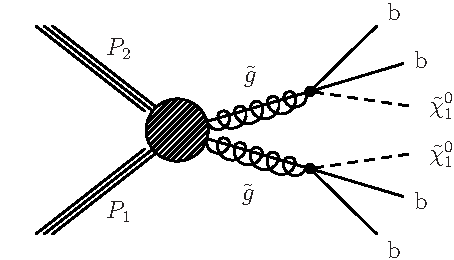
\includegraphics[width=0.3\textwidth]{figures/susyResults/T1bbbb_feyn}
      \label{fig:T1bbbb_feyn}
    } ~~
    \subfigure[T1tttt]{
      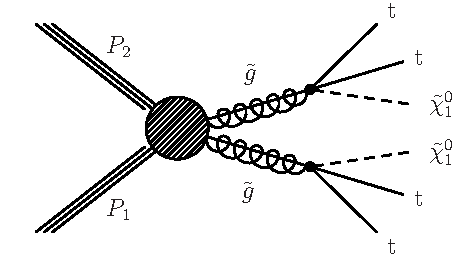
\includegraphics[width=0.3\textwidth]{figures/susyResults/T1tttt_feyn}
      \label{fig:T1tttt_feyn}
    } ~~
    % \subfigure[T1ttbb]{
    %   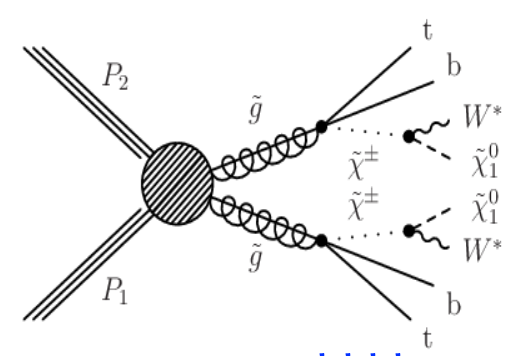
\includegraphics[width=0.3\textwidth]{figures/susyResults/T1ttbb_feyn.png}
    %   \label{fig:T1ttbb_feyn}
    % }
    \caption{
      Graphical representation of the production and decay of supersymmetric particles 
      in gluino models with decoupled third generation squarks. 
    }
    \label{fig:simplified-models-feyn-gluino}
  \end{center}
\end{figure}


%% \begin{figure}[h!]
%%   \begin{center}
%%     \subfigure[T5ttttDM175]{
%%       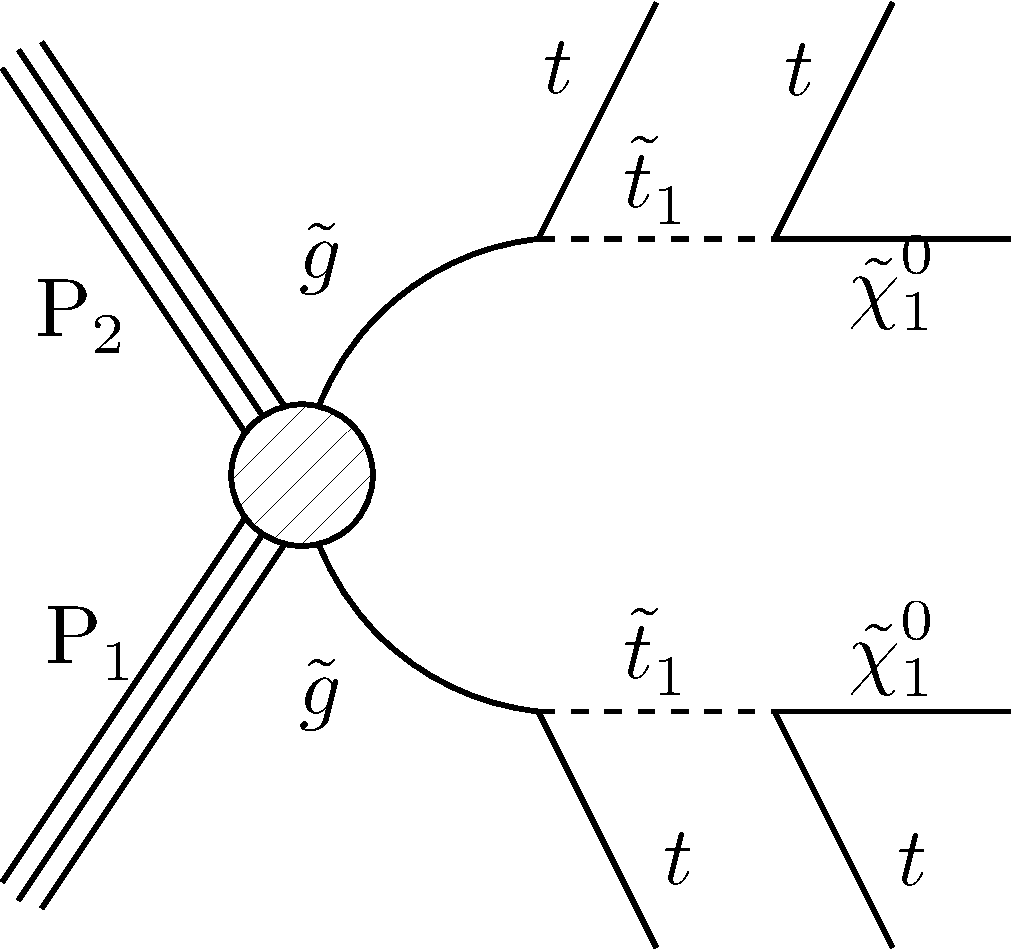
\includegraphics[width=0.3\textwidth]{figures/susyResults/T5ttttDM175_feyn}
%%       \label{fig:T5ttttDM175_feyn}
%%     } ~~
%%     \subfigure[T5tttt\_degen]{
%%       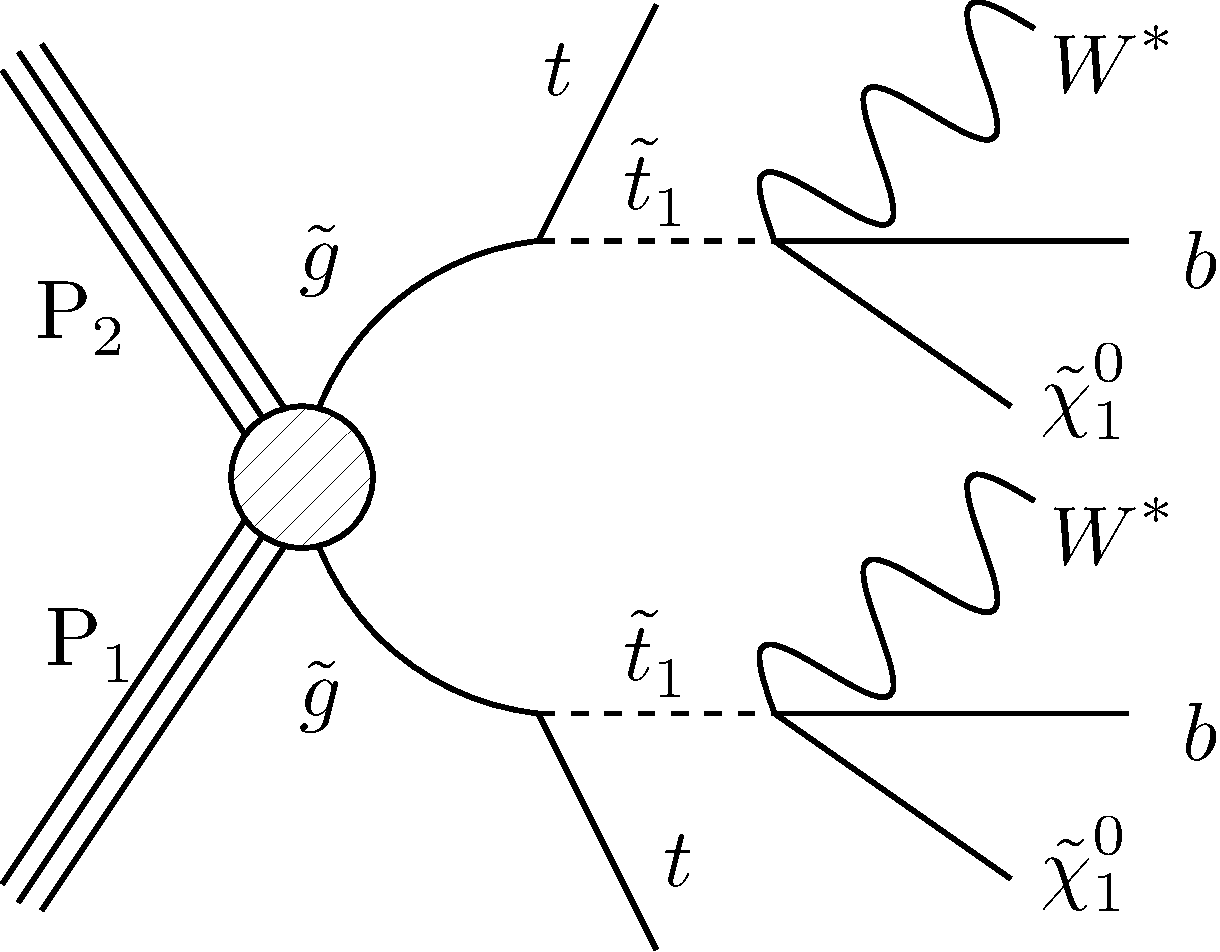
\includegraphics[width=0.3\textwidth]{figures/susyResults/T5tttt_degen_feyn}
%%       \label{fig:T5tttt_degen_feyn}
%%     } ~~
%%     \subfigure[T5ttcc]{
%%       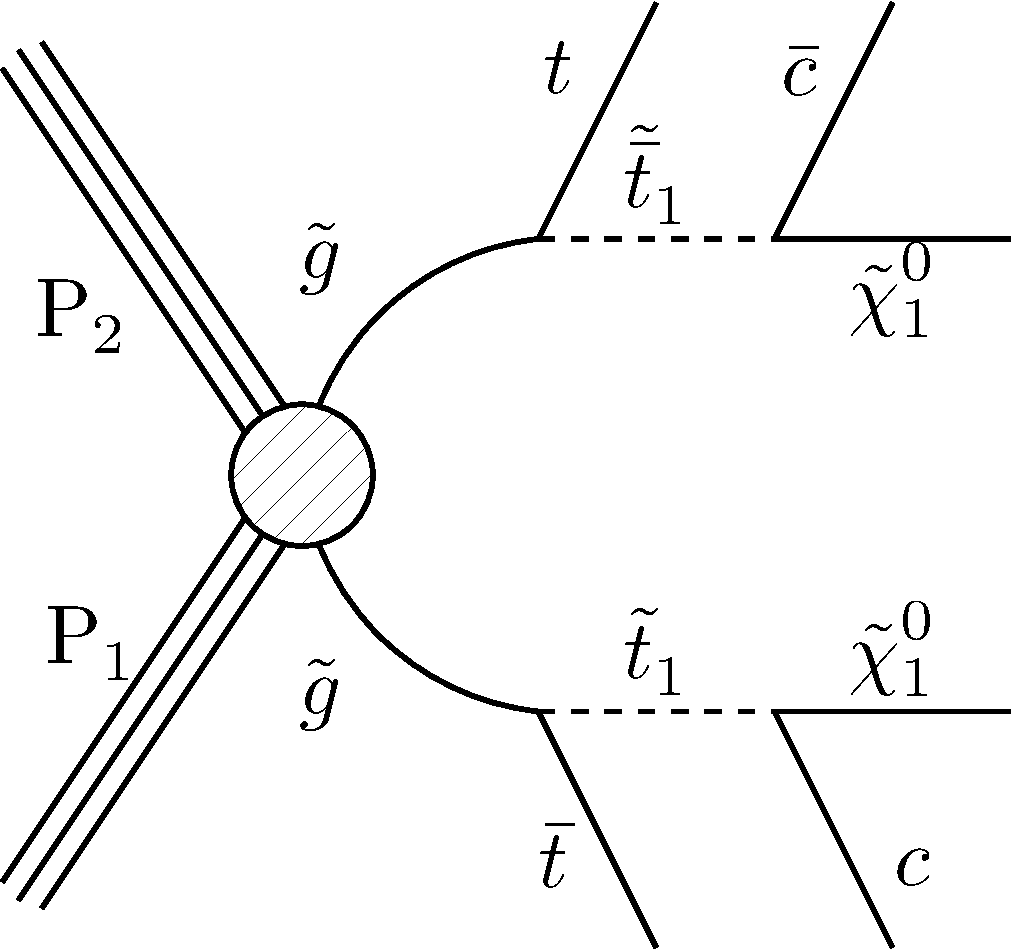
\includegraphics[width=0.3\textwidth]{figures/susyResults/T5ttcc_feyn}
%%       \label{fig:T5ttcc_feyn}
%%     }
%%     \caption{
%%       Graphical representation of the production and decay of supersymmetric particles 
%%       in gluino-mediated stop production, i.e. ``natural models''. 
%%     }
%%     \label{fig:simplified-models-feyn-natural}
%%   \end{center}
%% \end{figure}


\begin{figure}[h!]
  \begin{center}
    \subfigure[T1qqqq]{
      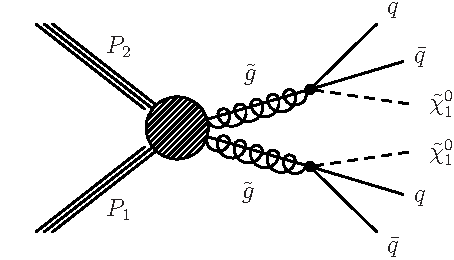
\includegraphics[width=0.3\textwidth]{figures/susyResults/T1qqqq_feyn}
      \label{fig:T1qqqq_feyn}
    } ~~
    \subfigure[T2qq]{
      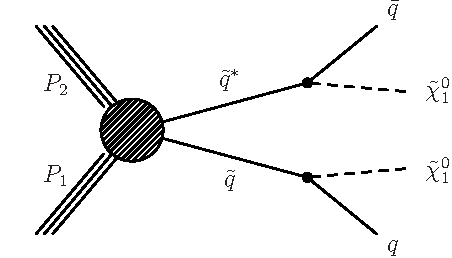
\includegraphics[width=0.3\textwidth]{figures/susyResults/T2qq_feyn}
      \label{fig:T2qq_feyn}
    }
    \caption{
      Graphical representation of the production and decay of supersymmetric particles 
      in ``light-flavour models'', i.e. with gluinos/squarks decaying to light quarks. 
    }
    \label{fig:simplified-models-feyn-light}
  \end{center}
\end{figure}


\begin{figure}[h!]
  \begin{center}
    \subfigure[T2tt]{
      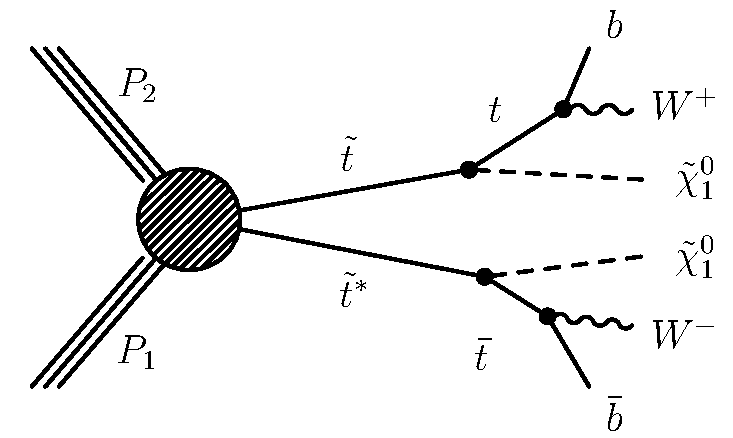
\includegraphics[width=0.3\textwidth]{figures/susyResults/T2tt_feyn}
      \label{fig:T2tt_feyn}
    } ~~
    % \subfigure[T2cc]{
    %   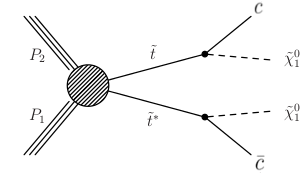
\includegraphics[width=0.3\textwidth]{figures/susyResults/T2cc_feyn}
    %   \label{fig:T2cc_feyn}
    % } \\
    % \subfigure[T2tb]{
    %   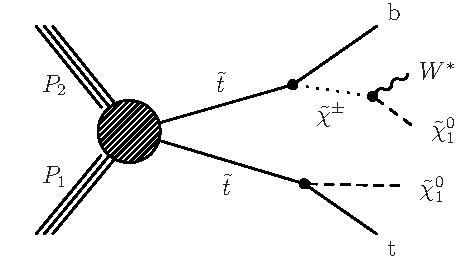
\includegraphics[width=0.3\textwidth]{figures/susyResults/T2tb_feyn}
    %   \label{fig:T2tb_feyn}
    % }~~
    % \subfigure[TbW\_X05]{
    %   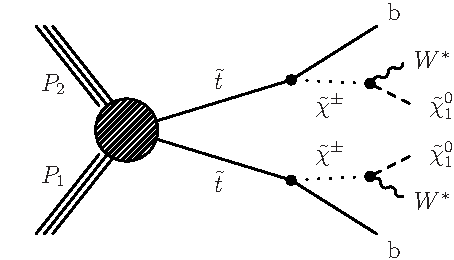
\includegraphics[width=0.3\textwidth]{figures/susyResults/T2bW_X05_feyn}
    %   \label{fig:T2bW_X05_feyn}
    % } \\
    \subfigure[T2bb]{
      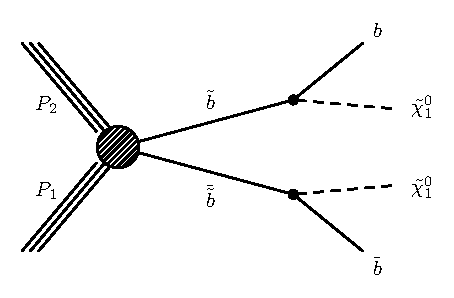
\includegraphics[width=0.3\textwidth]{figures/susyResults/T2bb_feyn}
      \label{fig:T2bb_feyn}
    }
    \caption{
      Graphical representation of the production and decay of supersymmetric particles 
      in models with the production of third generation squarks (stops and sbottoms). 
    }
    \label{fig:simplified-models-feyn-3rdGen}
  \end{center}
\end{figure}




%% \subsection{Signal acceptance and contamination}
%% \label{sec:sig-accept-contam}
%% In Tab. \ref{tab:sig-eff-bestCat} the signal efficiency for benchmark mass points for all the models is summarised, 
%% together with the 4 categories used in the limit setting, identified with the ranking procedure described in Sec.~\ref{sec:likelihood}. \\
%% The signal efficiency across the whole ($m_{\mathrm{Susy}},m_{\mathrm{LSP}}$) for the simplified models used in the analysis 
%% is shown in Fig.~\ref{fig:T1bbbb_eff}-\ref{fig:T2qq_eff}. 
%% The signal acceptance including only the 4 most sensitive jet multiplicity categories used to compute the exclusion 
%% is compared with the acceptance of the whole signal region of the analysis (see for example Fig.~\ref{fig:T1bbbb_eff_doubleRatio}). 
%% For models with high jet multiplicity (T1tttt,T1ttbb,T5tttt) almost 100\% of the acceptance is 
%% included in the $\geq5$ jet bin, and thus the restriction to 4 jet categories doesn't affect the signal efficiency 
%% because this bin is always among the most sensitive.  
%% For compressed models or, in general, models with low jet multiplicity (T2cc,T2-4bd) the signal regions with larger signal yield often are not 
%% selected among the top 4, due to the large background and poor sensitivity. 
%% In this case some efficiency loss are observed, for instance in Fig.~\ref{fig:T2cc_eff_doubleRatio},\ref{fig:T2-4bd_eff_doubleRatio}. 


%% \begin{table}[h!]
%%   \caption{
%%     Signal efficiency and list of the 4 most excluding jet multiplicity categories
%%     for compressed and uncompressed models used in the analysis.
%%   }
%%   \label{tab:sig-eff-bestCat}
%%   \centering
%%   \begin{tabular}{ lllll }
%%     \hline
%%     \hline
%%     Model & $(m_{\mathrm{Susy}},m_{\mathrm{LSP}})$ & Efficiency (4 best cat.) & Efficiency (total) & Cat. used for limits \\ 
%%     \hline
%%     \multirow{2}{*}{T1bbbb}
%%      & (1500,100) & 10.1\%  & 10.1\%  & $\geq5j,4j,3j,2j$ \\
%%      & (1000,800) & 4.9\%   & 7.5\%   & $\geq5j,4j,\geq5a,4a$ \\ \hline
%%     \multirow{2}{*}{T1tttt}
%%      & (1300,100) & 2.4\%   & 2.4\% & $\geq5j,\geq5a,4j,3j$ \\
%%      & (800,400)  & 0.6\%   & 0.6\% & $\geq5j,\geq5a,4j,4a$ \\ \hline
%%     \multirow{2}{*}{T1ttbb}
%%      & (1300,100) & 3.8\%   & 3.8\% & $\geq5j,4j,3j,\geq5a$ \\
%%      & (1000,700) & 3.4\%   & 4.0\% & $\geq5j,\geq5a,4j,3j$ \\ \hline
%%     \multirow{2}{*}{T5ttcc}
%%      & (1200,200) & 4.9\%   & 5.0\% & $\geq5j,4j,3j,\geq5a$ \\
%%      & (750,600)  & 1.0\%   & 1.4\% & $\geq5j,\geq5a,4j,4a$ \\ \hline
%%     \multirow{2}{*}{T5ttttDM175}
%%      & (800,100)  & 0.2\%   & 0.2\% & $\geq5j,\geq5a,3j,4j$ \\
%%      & (700,400)  & 0.2\%   & 0.3\% & $\geq5j,\geq5a,4j,1j$ \\ \hline
%%     \multirow{2}{*}{T5tttt\_degen}
%%      & (1100,100) & 1.3\%   & 1.3\% & $\geq5j,4j,3j,4a$ \\
%%      & (800,600)  & 1.9\%   & 2.5\% & $\geq5j,\geq5a,4a,4j$ \\ \hline
%%     \multirow{2}{*}{T2tt}
%%      & (700,50)   & 8.1\%   & 8.8\% & $\geq5j,4j,3j,\geq5a$ \\
%%      & (350,100)  & 1.4\%   & 1.9\% & $\geq5j,\geq5a,4a,4j$ \\ \hline
%%     T2cc & (325,305)   & 0.8\%   & 2.4\% & $\geq5j,4j,3j,2j$ \\ \hline
%%     T2-4bd & (300,290) & 0.9\%   & 2.7\% & $3j,4j,\geq5j,2j$ \\ \hline
%%     T2mixed & (300,250)& 0.4\%   & 1.3\% & $\geq5j,4j,\geq5a,4a$ \\ \hline
%%     \multirow{2}{*}{T2tb}
%%      & (600,50)   & 6.1\%   & 7.0\% & $\geq5j,4j,3j,2j$ \\
%%      & (350,225)  & 1.0\%   & 1.7\% & $\geq5j,4j,3j,3a$ \\ \hline
%%     \multirow{2}{*}{T2bW\_X05}
%%      & (400,100)  & 1.1\%   & 1.5\% & $\geq5j,4j,\geq5a,3j$ \\
%%      & (350,225)  & 0.3\%   & 0.5\% & $\geq5j,\geq5a,4j,4a$ \\ \hline           
%%     \multirow{2}{*}{T2bb}
%%      & (800,50)   & 1.5\%   & 1.6\% & $2j,3j,4j,\geq5j$ \\
%%      & (375,300)  & 0.1\%   & 0.2\% & $\geq5j,4j,3a,3j$ \\ \hline
%%     \multirow{2}{*}{T1qqqq}
%%      & (1300,100) & 9.4\%   & 9.4\% & $\geq5j,4j,3j,2j$ \\
%%      & (900,700)  & 5.6\%   & 8.2\% & $\geq5j,\geq5a,4j4a$ \\ \hline
%%     \multirow{2}{*}{T2qq}
%%      & (1050,100)   & 17.9\%   & 18.5\% & $\geq5j,3j,2j,4j$ \\
%%      & (650,550)  & 2.6\%   & 5.0\% & $\geq5j,4j,\geq5a,4a$ \\ \hline
%%      \hline
%%   \end{tabular}
%% \end{table}


%% The level of signal contamination in the control regions is expected to be negligible 
%% for most of the models that are targeted by this search. 
%% The requirement of one muon, two muons or one photon in the \mj, \mmj and \gj respectively 
%% ensures that the control regions are depleted from signal events, in the case where the final state is all-hadronic. 
%% The only partial exception is the gluino pair production and stop pair production followed by decay into top quarks, 
%% called T1tttt and T2tt respectively. 
%% In this case, when top decays leptonically, a residual signal contamination may be found in the muon control regions. 
%% However, the kinematic selection applied to the control regions, like the absence of any \alt cut and the $m_{T}$ cut, helps to reduce the signal contamination. \\
%% The metric that is chosen to study the signal contamination in the following is the double-ratio $(S_{SR}/B_{SR})/(S_{CR}/B_{CR})$, 
%% as the sensitivity of the control region ($S_{CR}/B_{CR}$) is expected to be small compared to the one in the signal region ($S_{SR}/B_{SR}$) by definition. 

%% Fig. ~\ref{fig:contamination_T2tt},\ref{fig:contamination_T2tt} characterises the level of signal
%% contamination for the T2tt ($m_{\mathrm{Stop}}=250$ GeV, $m_{\mathrm{LSP}}=50$ GeV) and 
%% T1tttt ($m_{\mathrm{Gluino}}=1400$ GeV, $m_{\mathrm{LSP}}=100$ GeV) models respectively, as a function of event category and
%% \scalht bin.
%% These two benchmark points have $m_{\mathrm{Susy}}-m_{\mathrm{LSP}} \sim m_{\mathrm{top}}$, which is the scenario 
%% where the largest signal contamination is expected, since the kinematics is similar to 
%% the top quark production, which is more likely to satisfy the control region selection with respect to the signal region. \\
%% Fig. ~\ref{fig:contamination_T2tt_yields_had} and ~\ref{fig:contamination_T2tt_yields_had} (\ref{fig:contamination_T1tttt_yields_had} and ~\ref{fig:contamination_T1tttt_yields_had}) show the
%% expected signal yield counts in the signal region and \mj control region respectively, for the T2tt (T1tttt) benchmark model. 
%% Fig. ~\ref{fig:contamination_T2tt_relEff} (~\ref{fig:contamination_T1tttt_relEff}) shows the ratio of signal contamination to signal efficiency of the signal region, for the T2tt (T1tttt) benchmark model. 
%% Fig. ~\ref{fig:contamination_T2tt_doubleRatio} (~\ref{fig:contamination_T1tttt_doubleRatio}) shows the ratio of sensitivity in the control region to the sensitivity in the signal region, for T2tt (T1tttt) benchmark model. The sensitivity is defined as the ratio of signal to background expected counts. 

%% \begin{figure}[h!]
%%   \begin{center}
%%     \subfigure[Expected counts in the signal region]{
%%       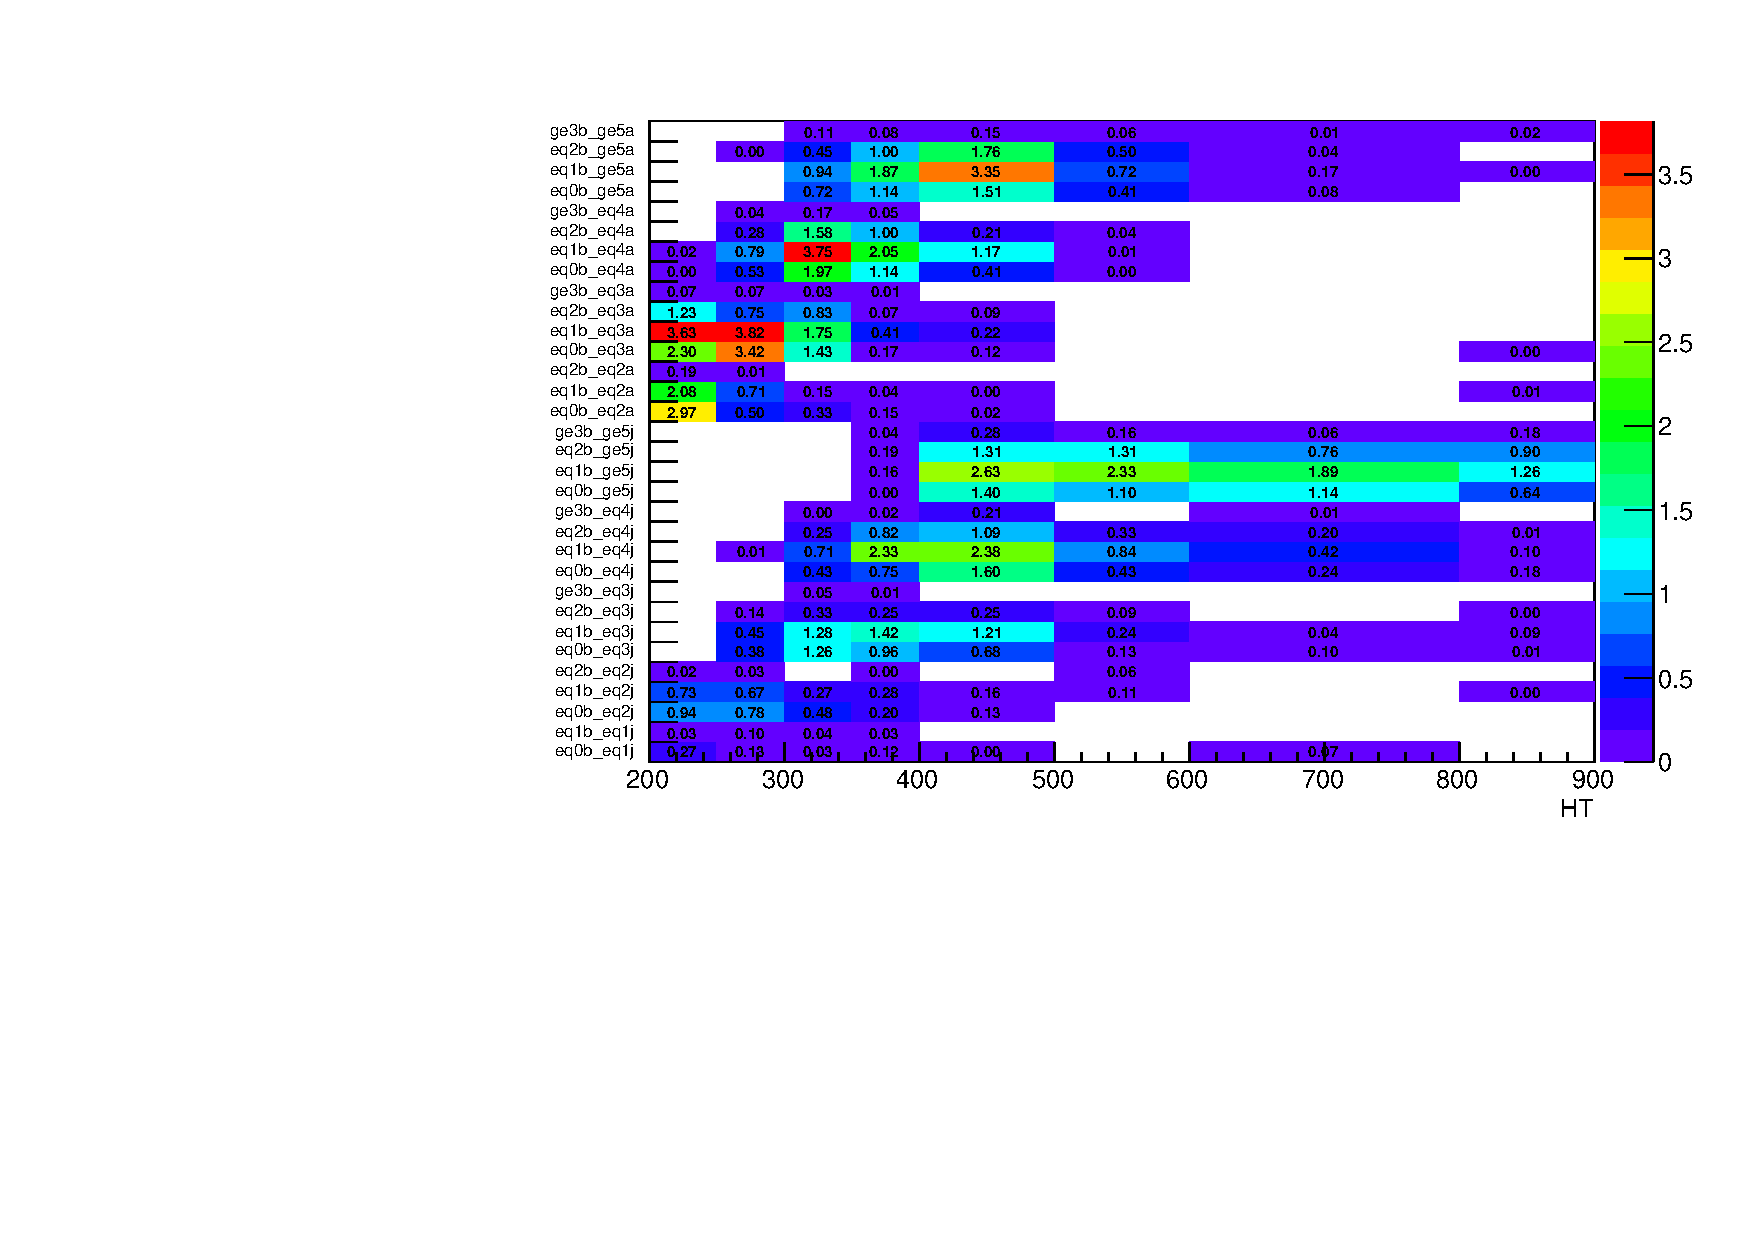
\includegraphics[width=0.5\textwidth]{figures/susyResults/sigYields_had_SMS-T2tt_mStop-250_mLSP-50_25ns}
%%       \label{fig:contamination_T2tt_yields_had}
%%     } 
%%     \subfigure[Expected counts in the \mj control region]{
%%       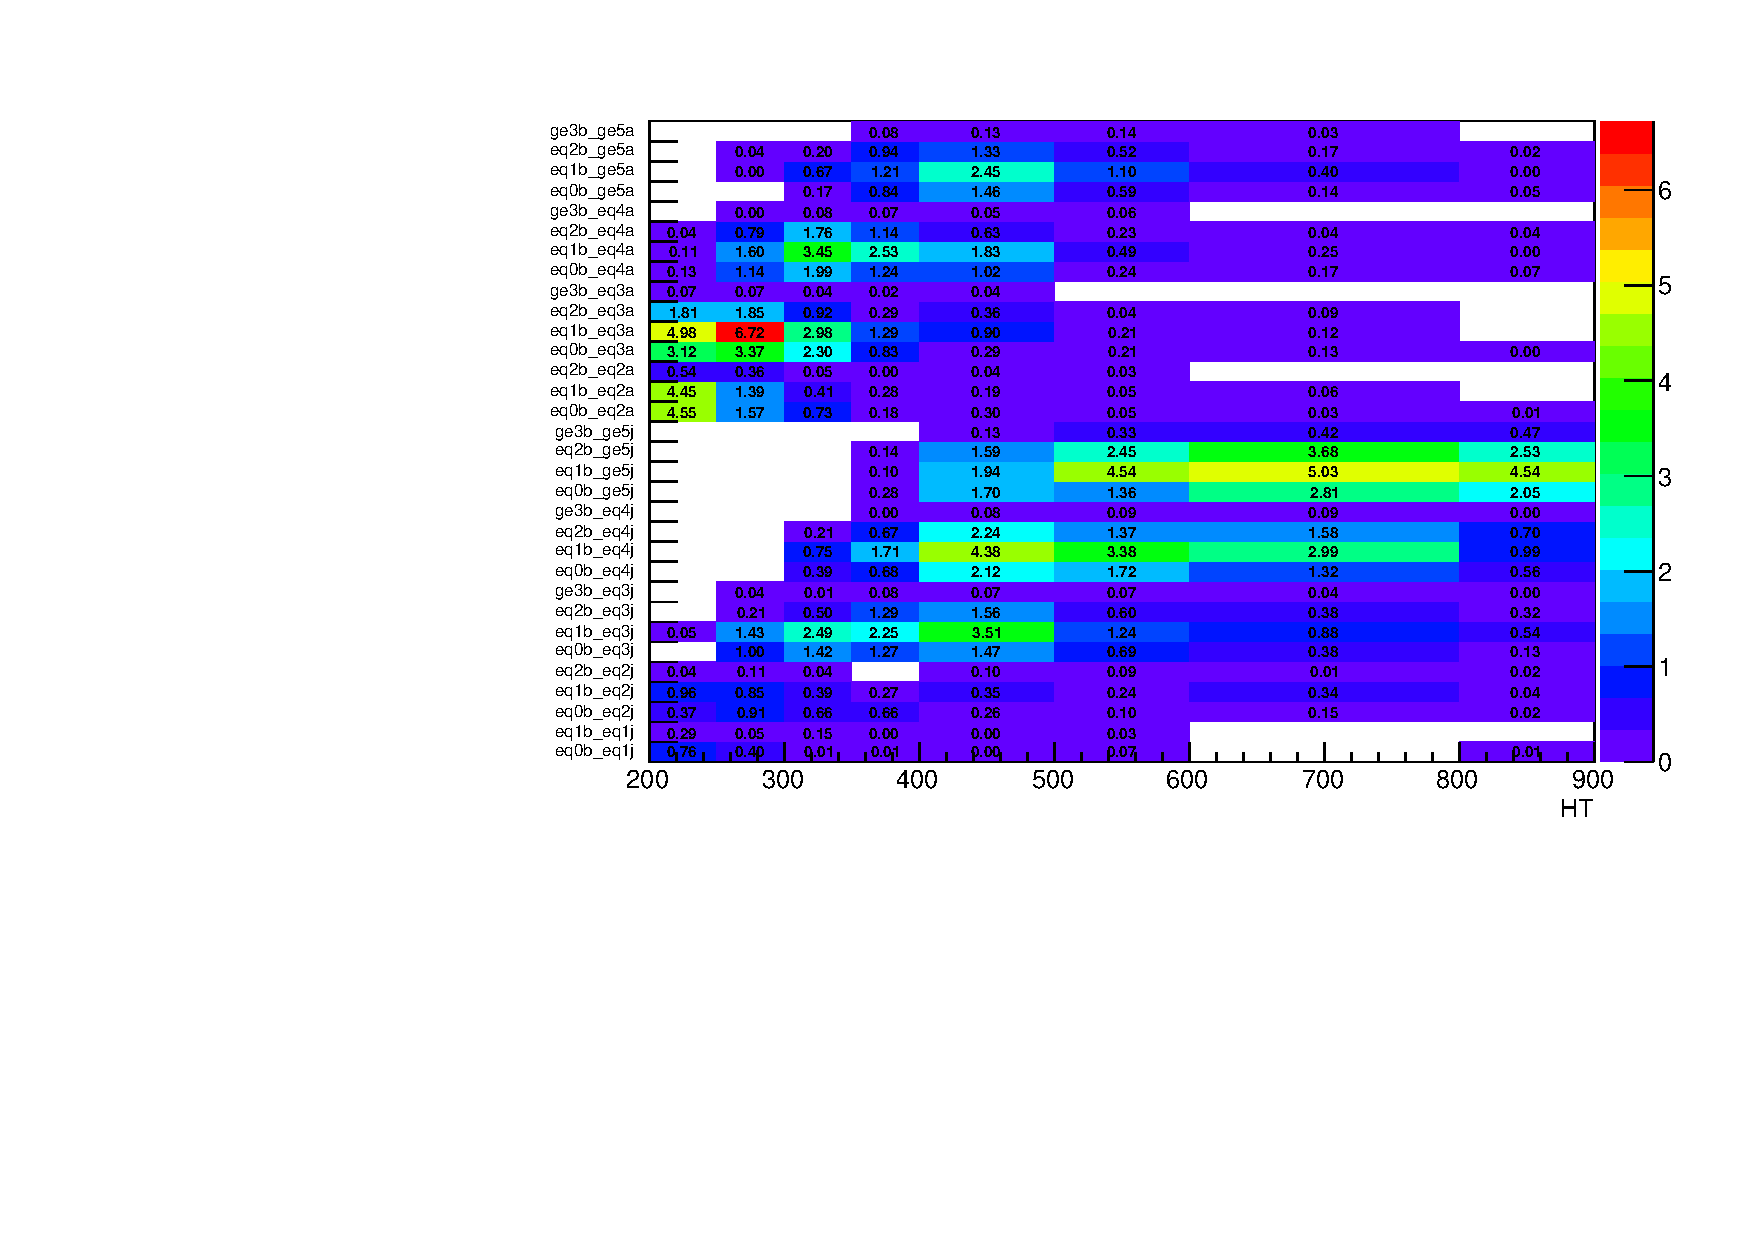
\includegraphics[width=0.5\textwidth]{figures/susyResults/sigYields_SingleMu_SMS-T2tt_mStop-250_mLSP-50_25ns}
%%       \label{fig:contamination_T2tt_yields_mj}
%%     } \\
%%     \subfigure[Ratio of signal acceptance (\mj to signal region)]{
%%       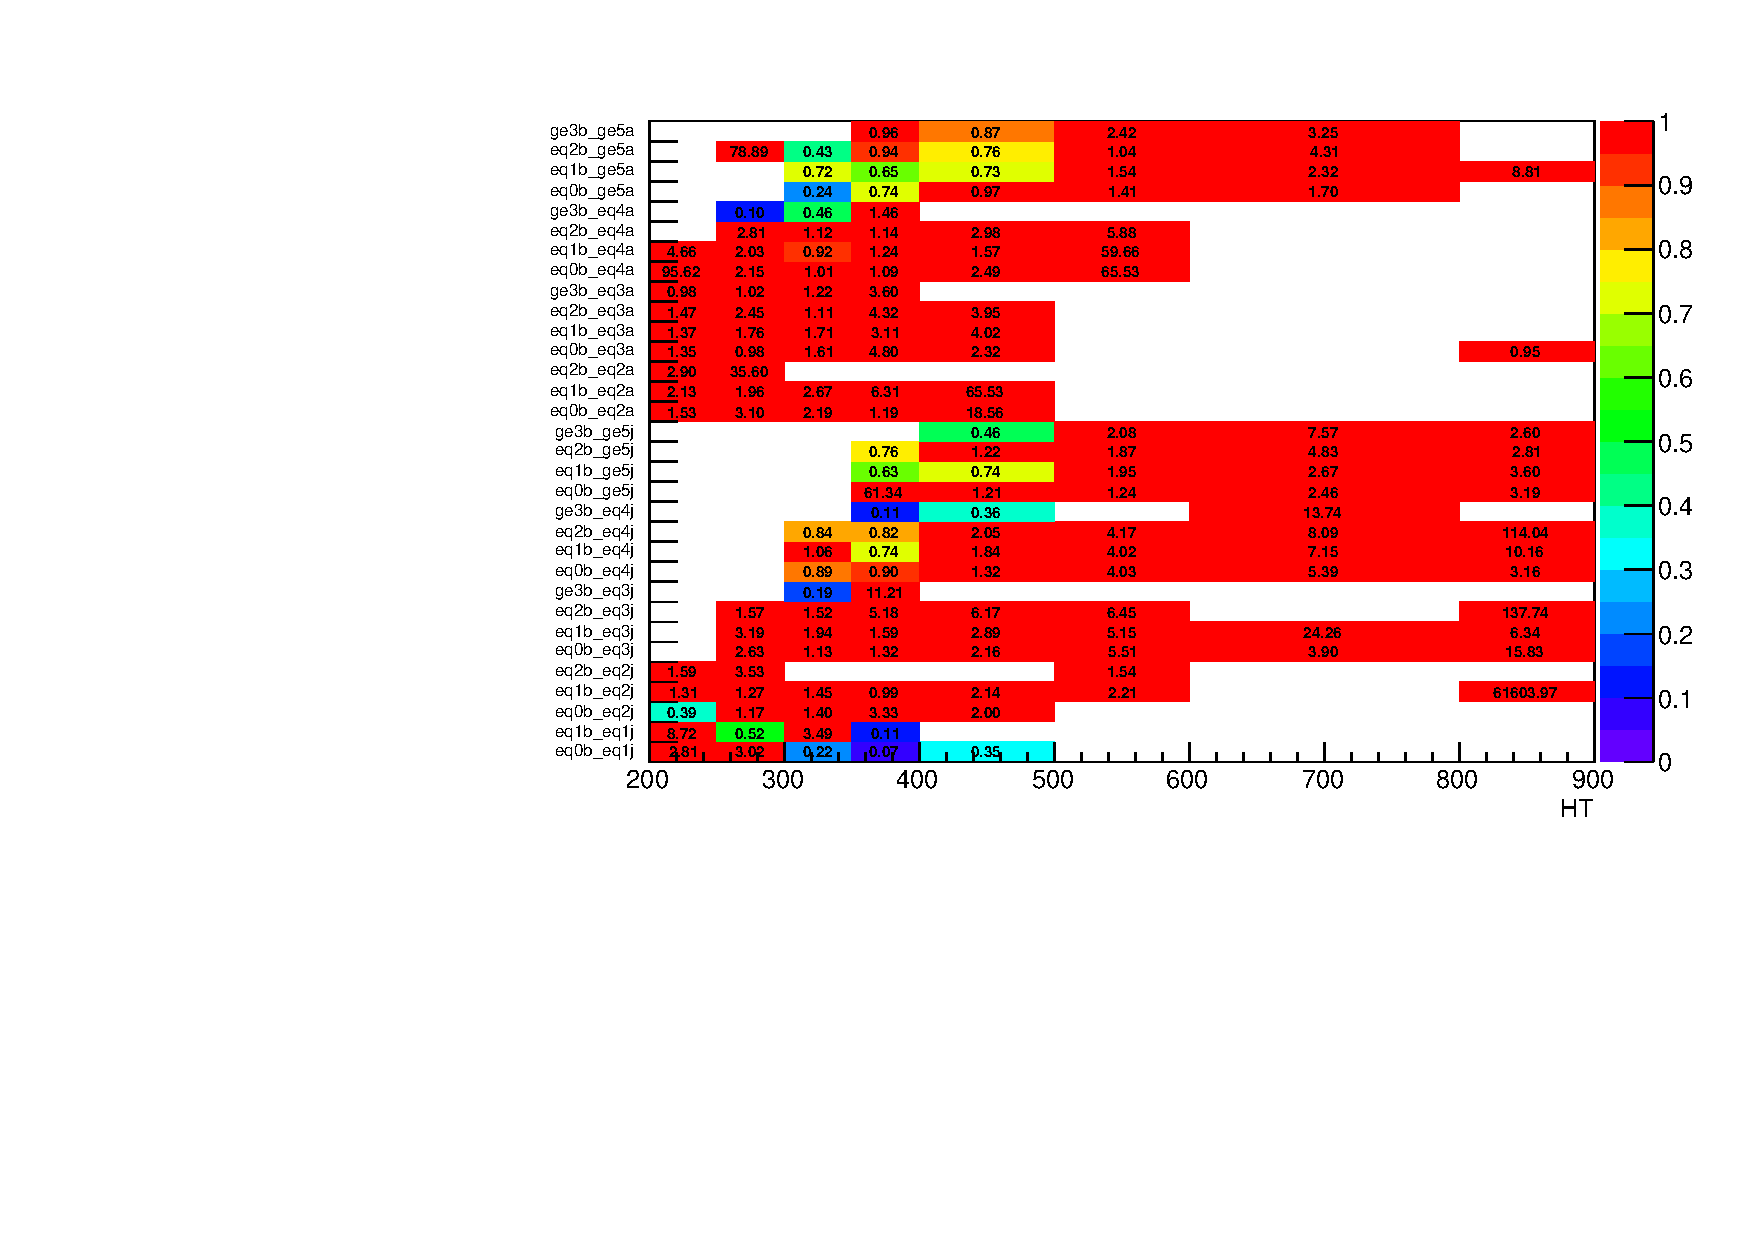
\includegraphics[width=0.5\textwidth]{figures/susyResults/relEff_SingleMu_SMS-T2tt_mStop-250_mLSP-50_25ns}
%%       \label{fig:contamination_T2tt_relEff}
%%     }
%%     \subfigure[Ratio of S/B values (\mj to signal region)]{
%%       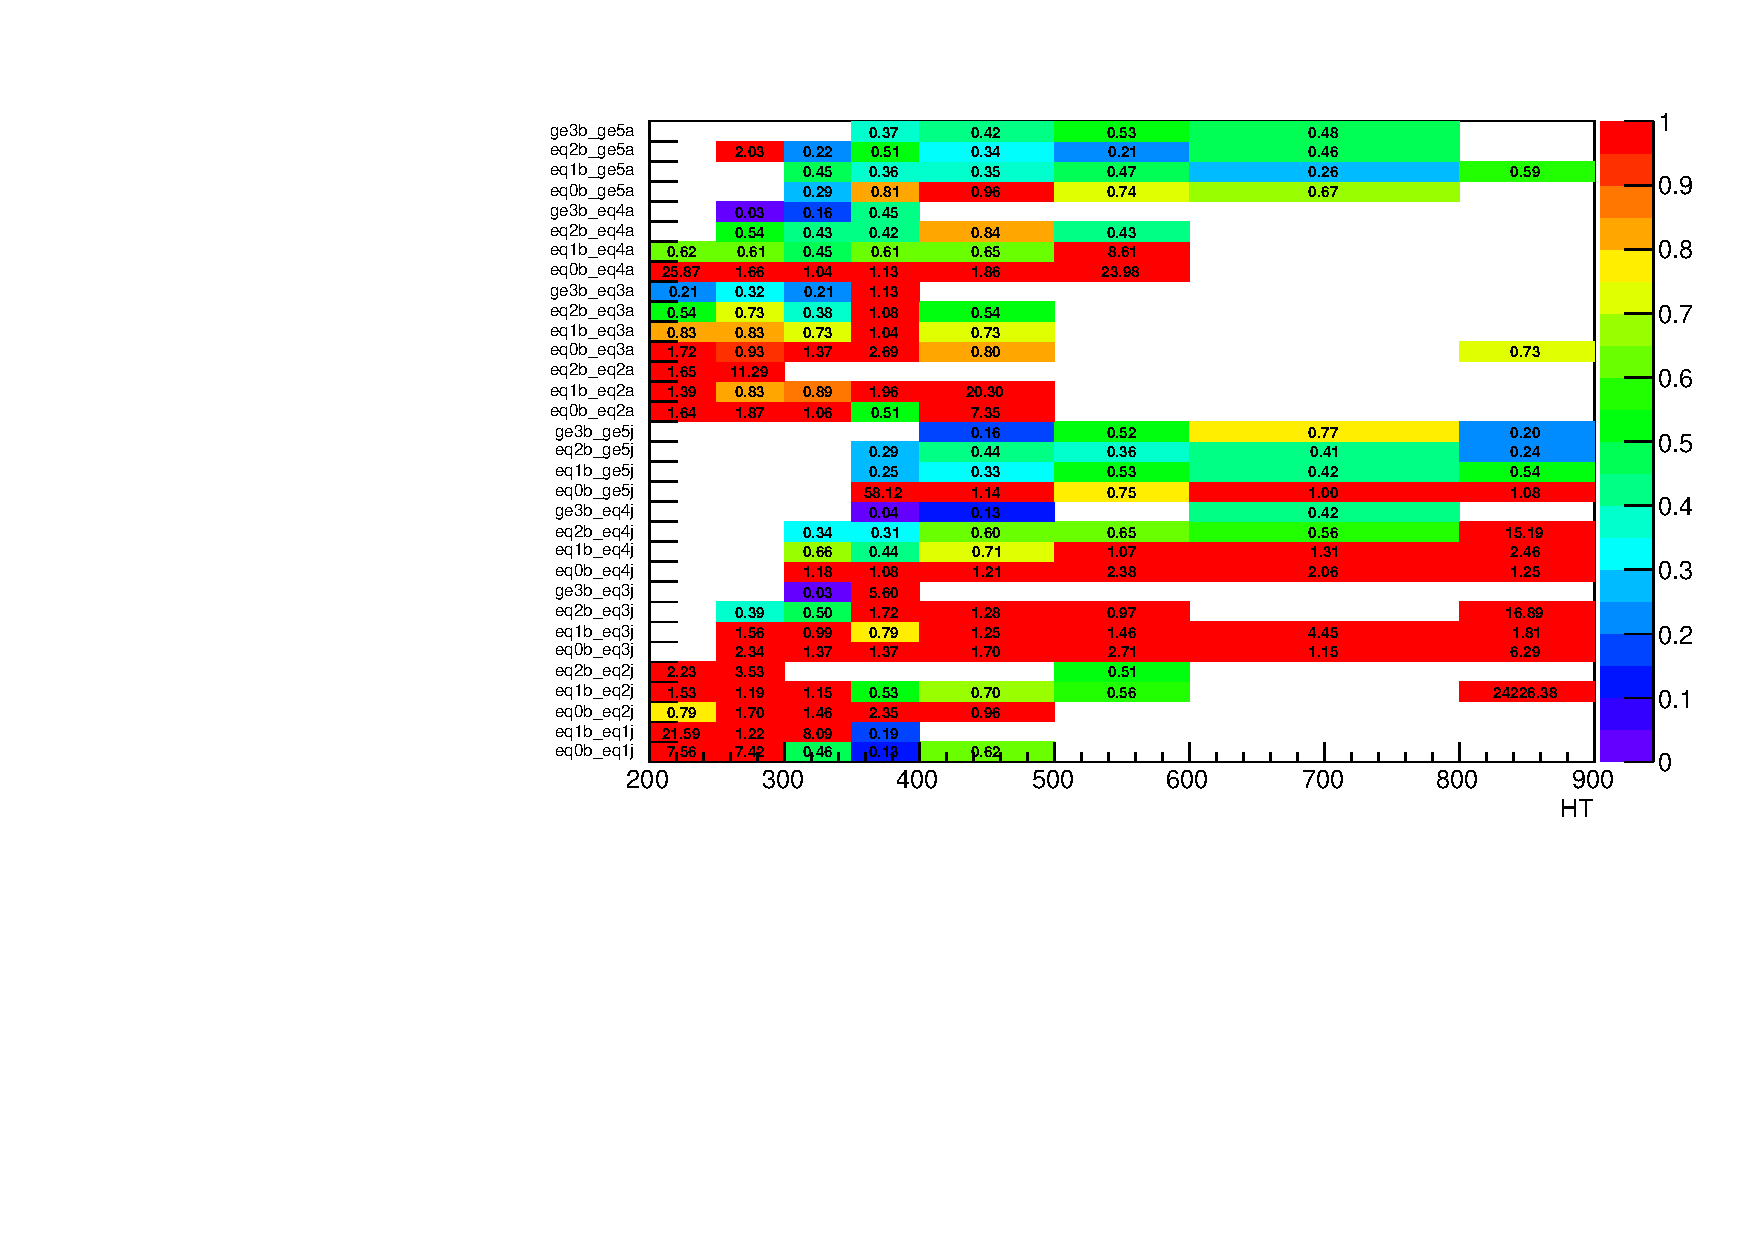
\includegraphics[width=0.5\textwidth]{figures/susyResults/doubleRatio_SingleMu_SMS-T2tt_mStop-250_mLSP-50_25ns}
%%       \label{fig:contamination_T2tt_doubleRatio}
%%     }
%%     \caption{Characterisation of signal acceptance and contamination
%%       in the signal and \mj control regions, respectively, for the
%%       benchmark model T2tt (250,50).}
%%     \label{fig:contamination_T2tt}
%%   \end{center}
%% \end{figure}

%% %% Figure~\ref{fig:contamination} (c) shows the ratio of these expected
%% %% yields (signal region with respect to the \mj control region). The
%% %% ratio is typically small, at the percent level for the most sensitive
%% %% categories (\ie with four or more jets and one or two b-tagged jets).

%% %% In addition, the event counts from SM background processes in the \mj
%% %% control sample are significantly higher than in the signal region, as
%% %% no \alphat requirement is made for the \mj sample. Therefore, the S/B
%% %% ratios for the signal region relative to the \mj sample are larger by
%% %% many factors, typically $\gg$10. Figure~\ref{fig:contamination} (d)
%% %% shows the ratio of S/B$_{\rm signal}$ over S/B$_{\rm \mj}$ as a
%% %% function of the event category and \scalht bin.

%% %% Figure~\ref{fig:contamination_T1tttt} characterises the level of
%% %% signal contamination in the \mj control sample for the benchmark model
%% %% T1tttt ($m_{\mathrm{Gluino}}=1400$ GeV, $m_{\mathrm{LSP}}=100$ GeV). A larger level of contamination is
%% %% expected for this model (with respect to T2tt), due to the
%% %% presence of four W bosons produced in the decay of the gluino-pair
%% %% system (via off-shell top squarks). The ratio of yields in the signal
%% %% and \mj control regions is at the level of $\sim$10--20\% for the most
%% %% sensitive categories (\ie with four or more jets, two or more b-tagged
%% %% jets, and at high \scalht). The ratio of S/B values for the signal
%% %% region relative to the \mj sample is still large, typically $\gg$10.

%% \begin{figure}[h!]
%%   \begin{center}
%%     \subfigure[Expected counts in the signal region]{
%%       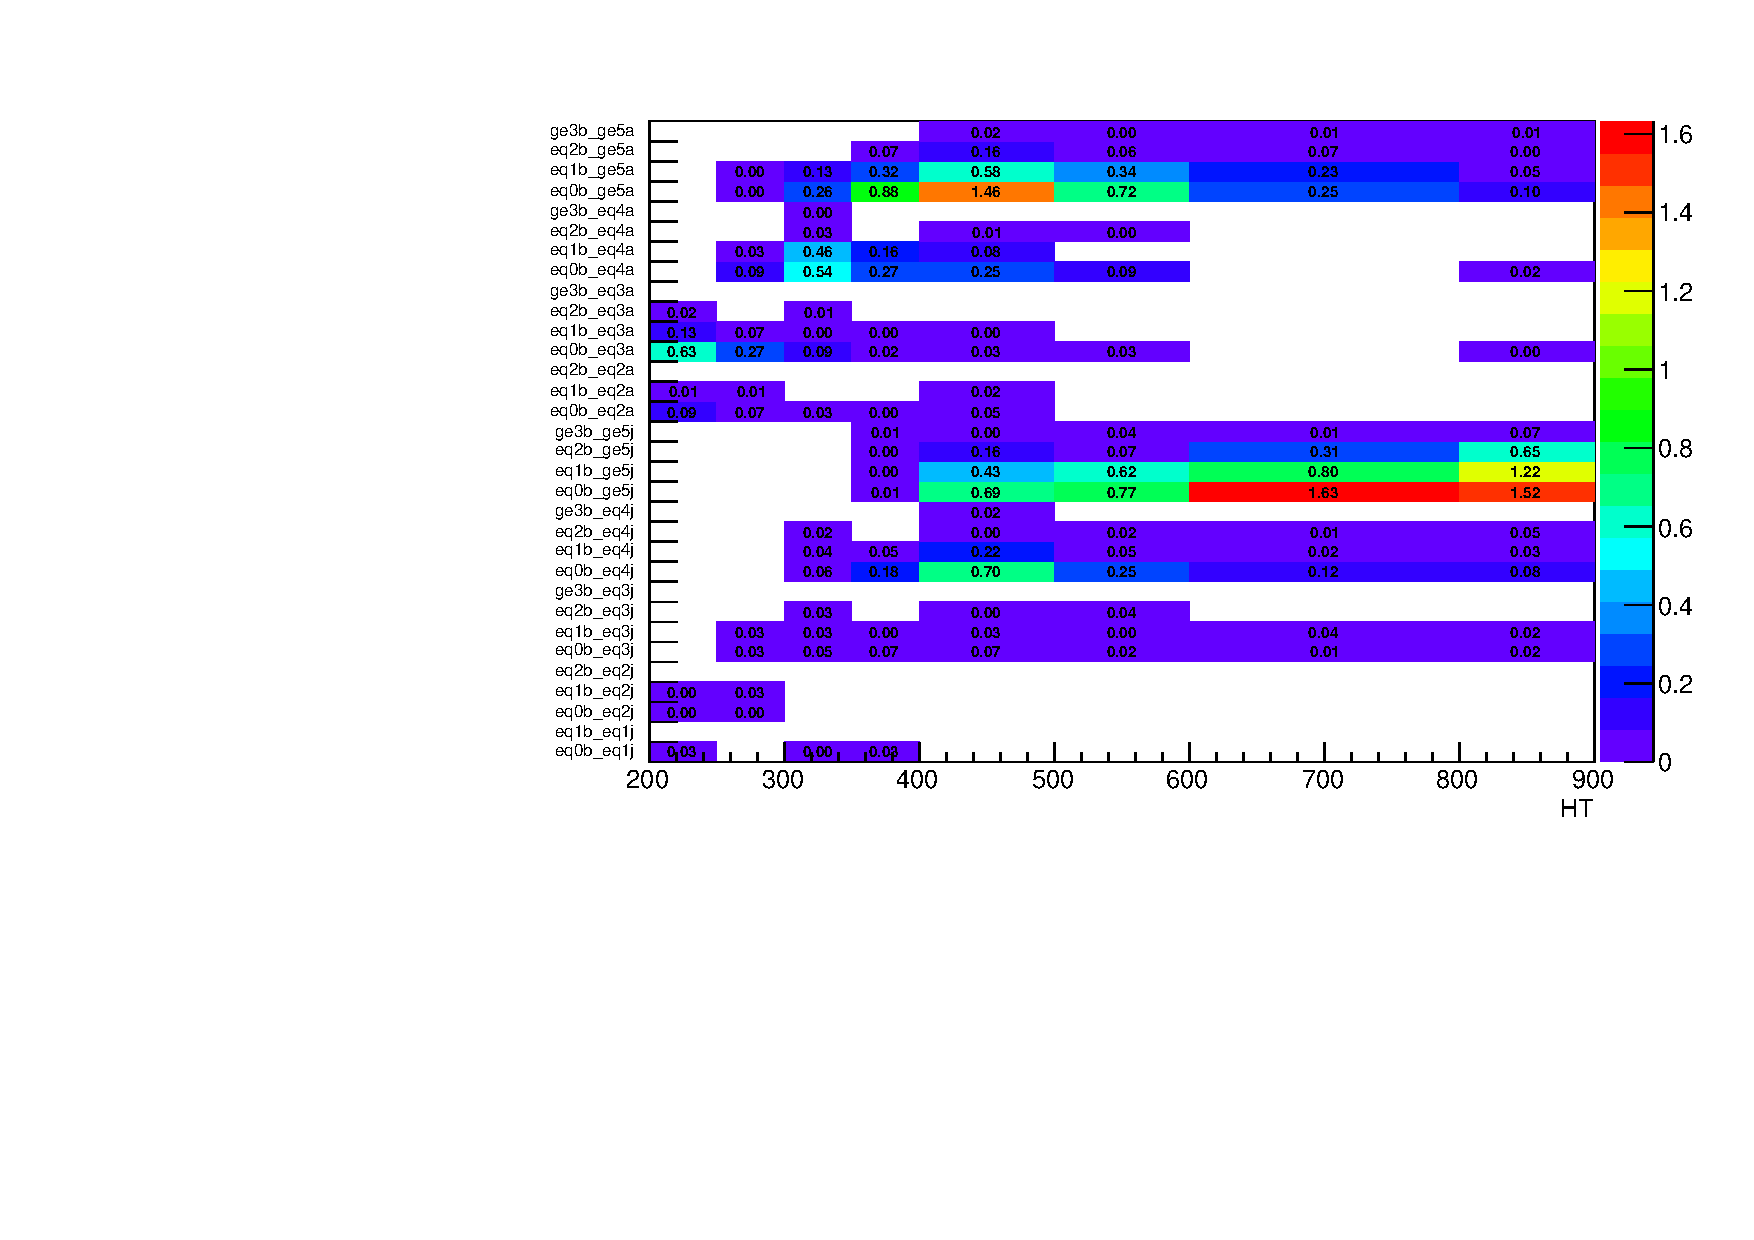
\includegraphics[width=0.5\textwidth]{figures/susyResults/sigYields_had_SMS-T1tttt_mGluino-800_mLSP-575_25ns}
%%       \label{fig:contamination_T1tttt_yields_had}
%%     } 
%%     \subfigure[Expected counts in the \mj control region]{
%%       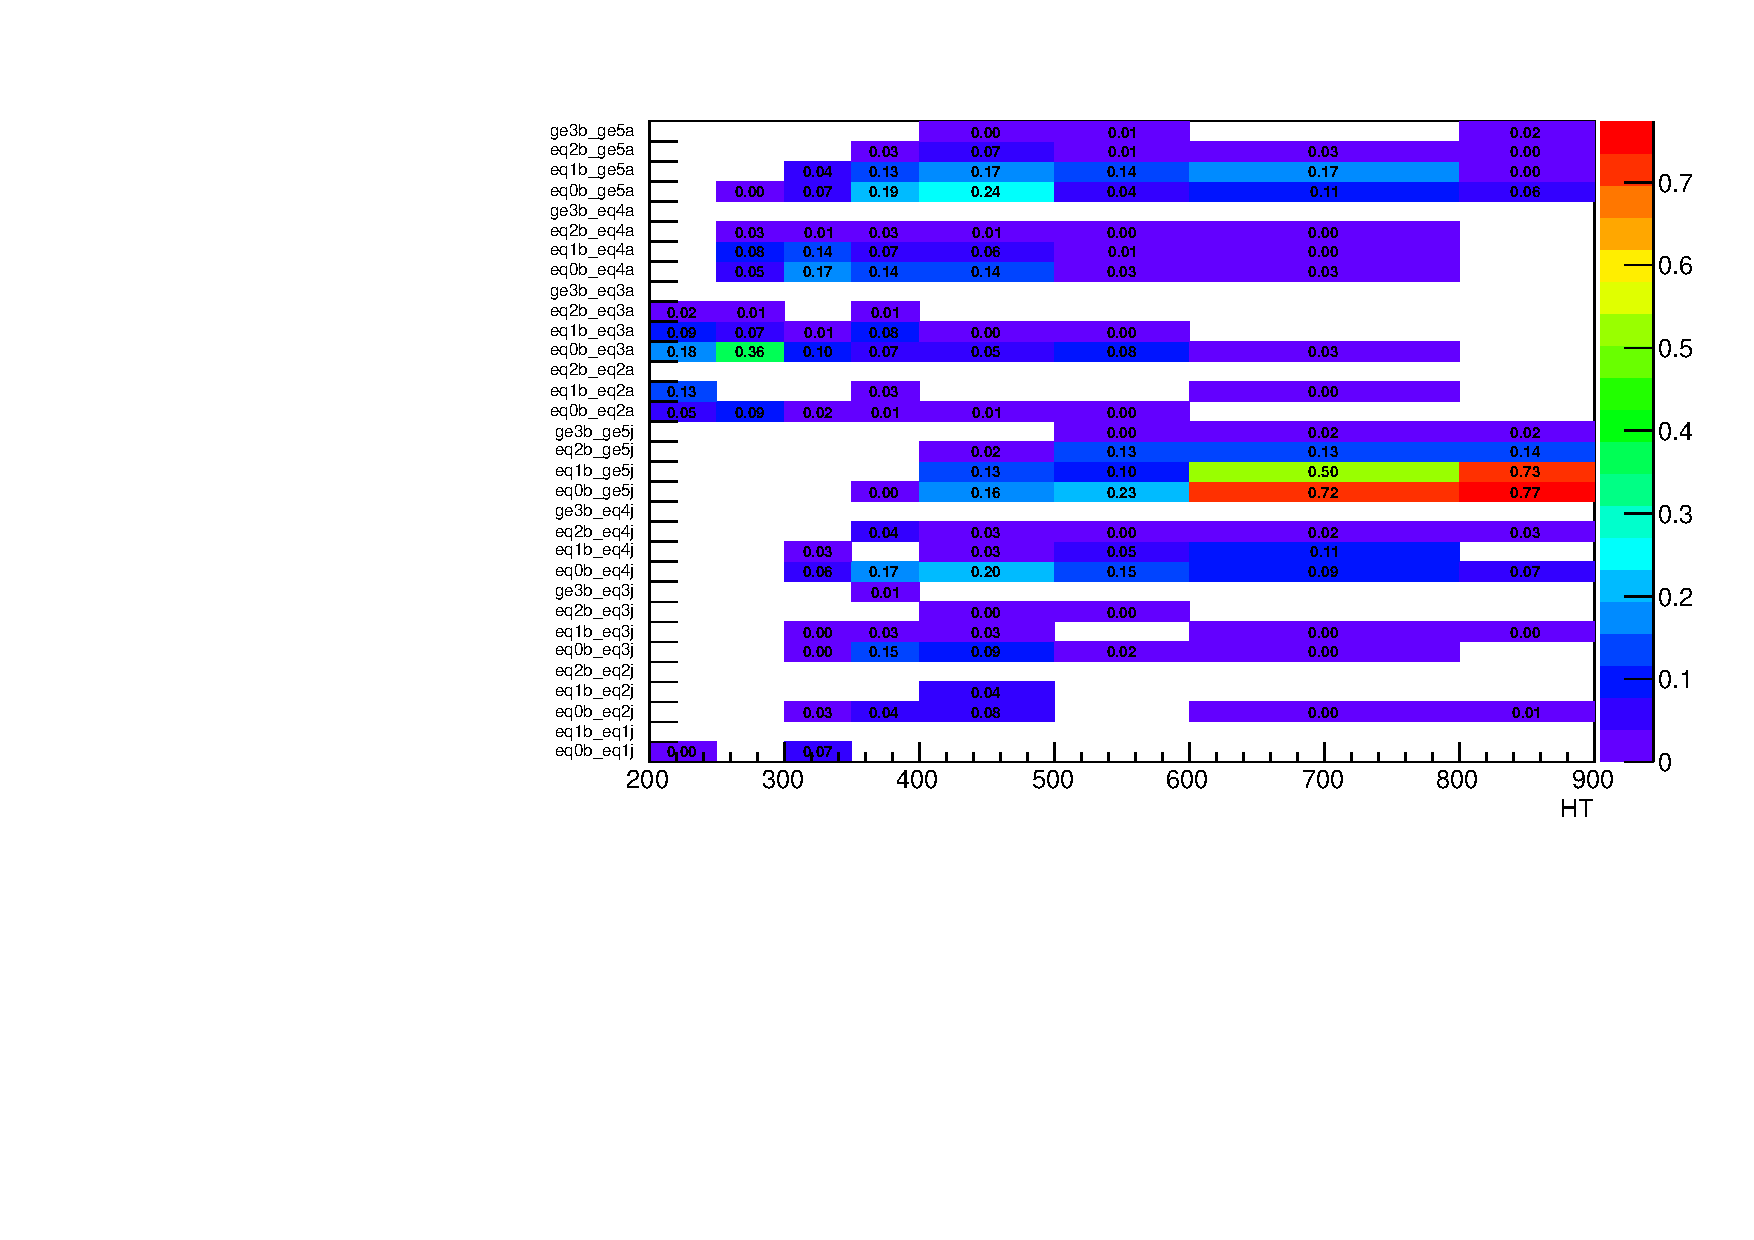
\includegraphics[width=0.5\textwidth]{figures/susyResults/sigYields_SingleMu_SMS-T1tttt_mGluino-800_mLSP-575_25ns}
%%       \label{fig:contamination_T1tttt_yields_mj}
%%     } \\
%%     \subfigure[Ratio of signal acceptance (\mj to signal region)]{
%%       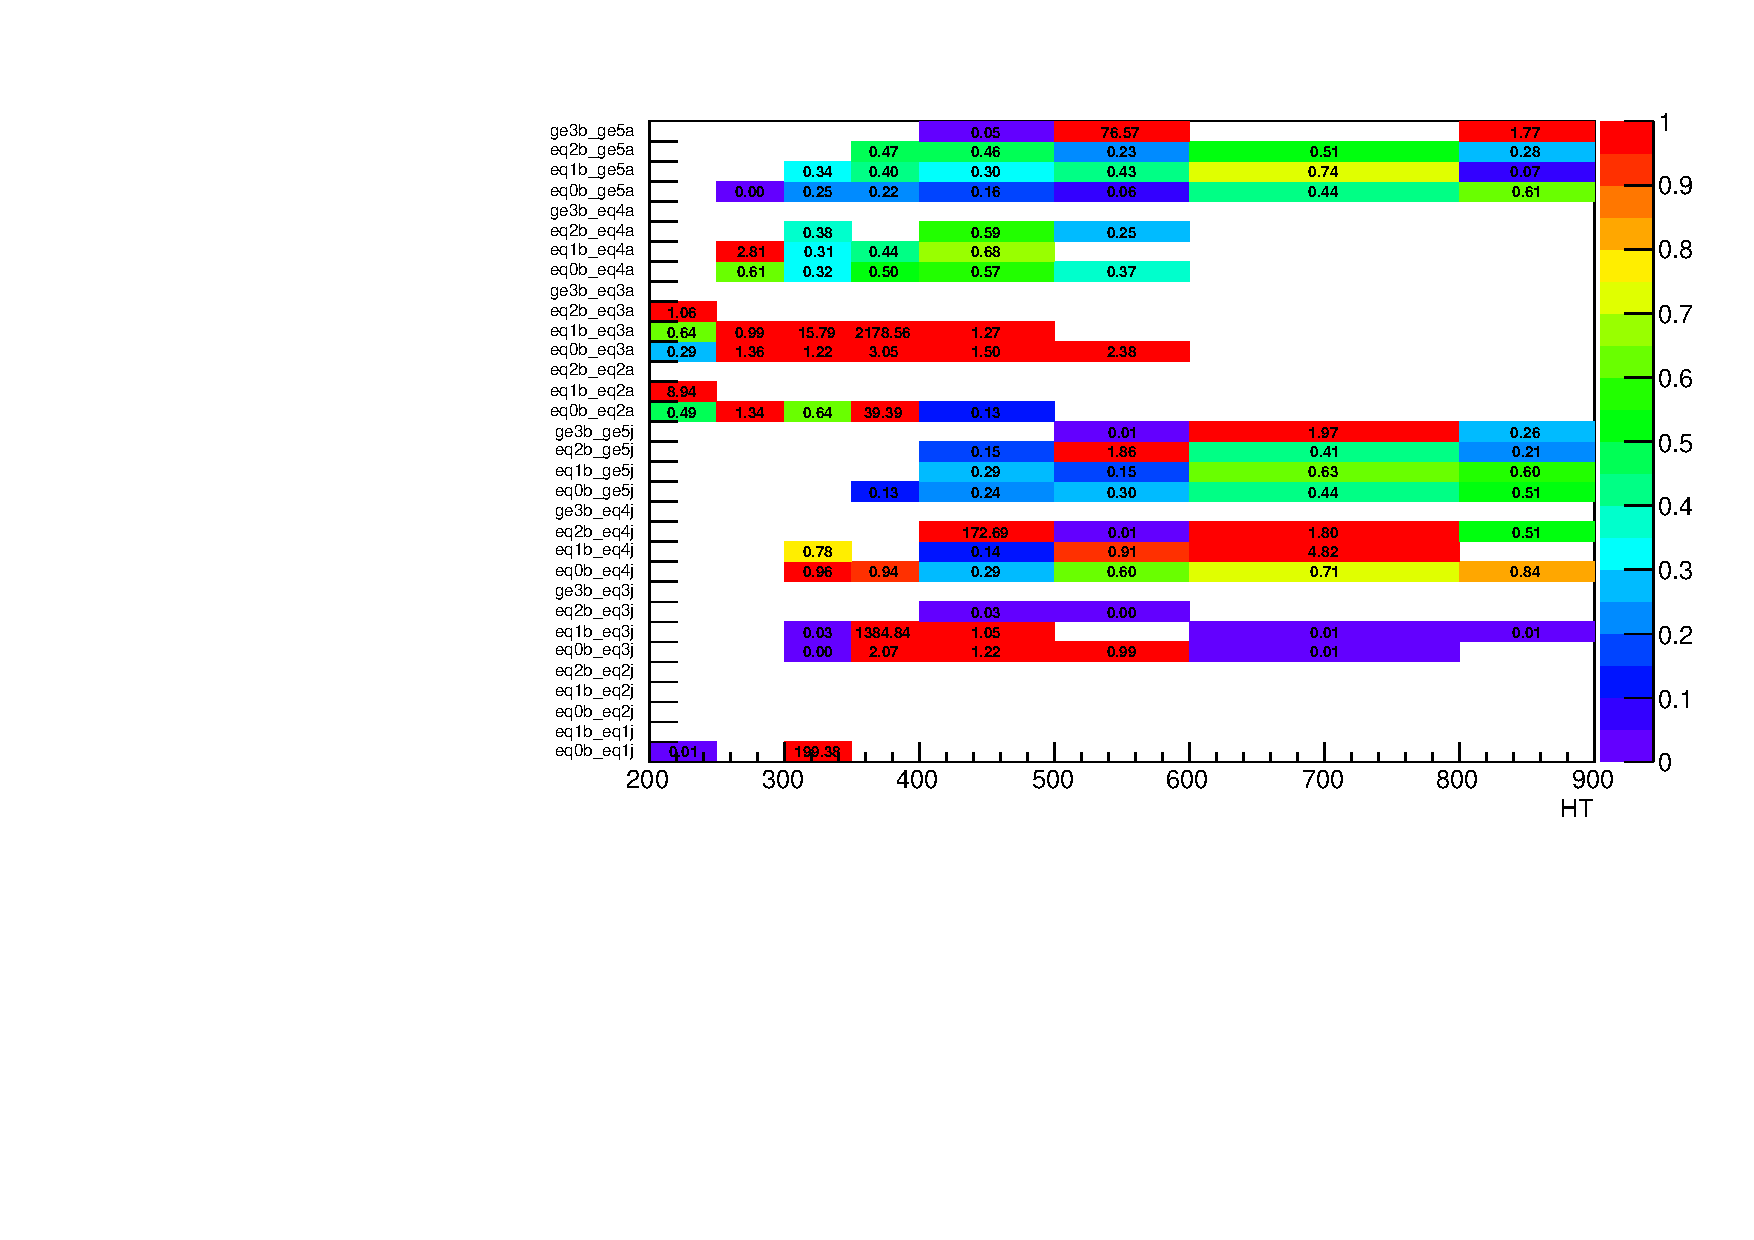
\includegraphics[width=0.5\textwidth]{figures/susyResults/relEff_SingleMu_SMS-T1tttt_mGluino-800_mLSP-575_25ns}
%%       \label{fig:contamination_T1tttt_relEff}
%%     }
%%     \subfigure[Ratio of S/B values (\mj to signal region)]{
%%       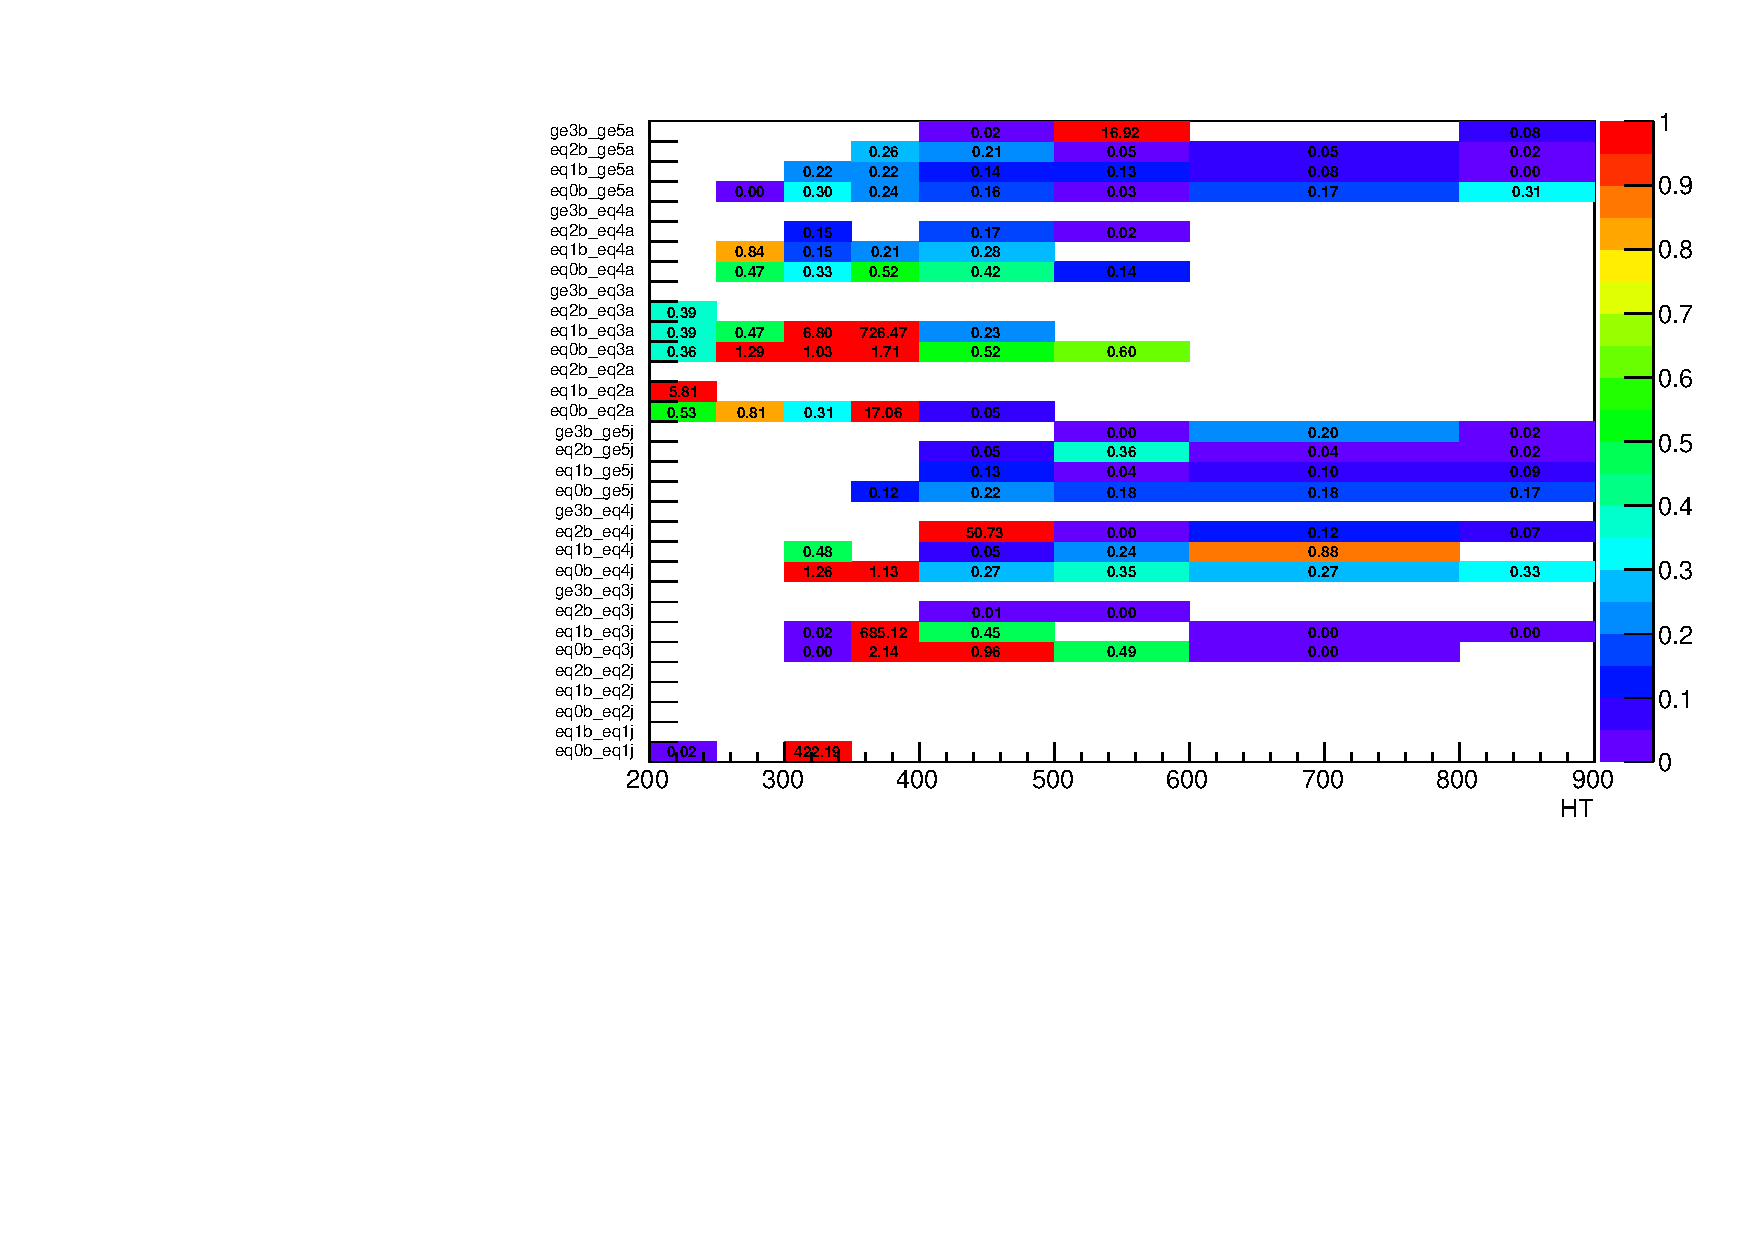
\includegraphics[width=0.5\textwidth]{figures/susyResults/doubleRatio_SingleMu_SMS-T1tttt_mGluino-800_mLSP-575_25ns}
%%       \label{fig:contamination_T1tttt_doubleRatio}
%%     }
%%     \caption{Characterisation of signal acceptance and contamination
%%       in the signal and \mj control regions, respectively, for the
%%       benchmark model T1tttt (800,575).}
%%     \label{fig:contamination_T1tttt}
%%   \end{center}
%% \end{figure}

%% The effect of signal contamination can be sizeable in these particular scenario for T2tt, 
%% as shown in Fig.~\ref{fig:contamination_T2tt_doubleRatio}, where in the most sensitive bins 
%% (high \nb, high \nj) the contribution of the control region sensitivity is comparable to 
%% the one of the signal region. However this is not an issue in the analysis, as 
%% the potential for signal contamination in all control samples
%% is fully accounted for in the likelihood model used to extract
%% the statistical interpretation (see Sec.~\ref{sec:likelihood}). 

%% For both models the level of contamination for the
%% \mmj sample is smaller still due to the requirement of a second
%% muon. The contamination for the \gj sample is expected to be zero for
%% the models under consideration. 

\subsection{Systematic uncertainties on signal efficiency times acceptance}
\label{sec:sig-syst}
The following sources of systematic uncertainty are propagated to the signal acceptance and shape, 
according to the recommendations agreed on within the collaboration. 
%% Relative effect on the yields are presented in Tab.~\ref{tab:sig-systematics} for some benchmark models. 

\begin{itemize}
  \item Luminosity: 6.2 \%, taken as correlated across all bins.
  \item Trigger: systematic measured using the difference between the electron and muon
  reference triggers (see Sec.~\ref{sec:triggers}). 
  \item MC statistics:  uncorrelated bin-by-bin uncertainty, affecting the shape of the signal. 
  \item Pileup reweighting: 5\% uncertainty on the minimum bias cross section (see Sec.~\ref{sec:pileup-reweighting}).
  \item b-tag efficiency: uncertainties on the FullSim and FastSim b-tag scale factors are propagated and taken as correlated across the bins. These are uncorrelated for mis-tag and efficiency systematics.
  \item Lepton efficiency: uncertainty on the lepton scale factors is propagated and taken as correlated across the bins. 
  \item Jet energy scale: uncertainty on the jet energy corrections is propagated and taken as correlated across the bins.
  \item Initial State Radiation (ISR): A systematic of half the correction factor applied to the MC per number of ISR jets is taken as correlated across the bins.
\end{itemize}



%% \begin{table}[h!]
%%   \caption{Representative range of uncertainty across the analysis bins 
%%     for each source of signal systematic.
%%     Two benchmark point are chosen for each model, 
%%     corresponding to ``compressed'' and ``uncompressed'' scenarios, 
%%     i.e. with small and large mass splitting between the mother particle and the LSP.
%%   }
%%   \label{tab:sig-systematics}
%%   \centering
%%   \begin{tabular}{ ccccccccc }
%%     \hline
%%     \hline
%% Model & ($m_{\mathrm{Susy}},m_{\mathrm{LSP}}$) & Luminosity & ISR & JEC & PU & b-tag & Trigger & MC stat. \\ \hline
%% \multirow{2}{*}{T1bbbb}
%%  & (1500,100) & 4.6\% & 1-2\% & 1-12\% & 1-4\% & 2-22\% & 1-3\% & 5-17\% \\ 
%%  & (1000,800) & 4.6\% & 1-17\% & 1-40\% & 1-20\% & 1-14\% & 1-15\% & 8-31\% \\ \hline 
%% \multirow{2}{*}{T1tttt}
%%  & (1300,100) & 4.6\% & 1-2\% & 2-7\% & 1-4\% & 2-12\% & 1-3\% & 7-16\% \\ 
%%  & (800,400) & 4.6\% & 1-2\% & 3-45\% & 1-13\% & 1-8\% & 1-10\% & 7-27\% \\ \hline 
%% \multirow{2}{*}{T1ttbb}
%%  & (1300,100) & 4.6\% & 1-2\% & 3-16\% & 1-18\% & 2-19\% & 1-4\% & 9-32\% \\ 
%%  & (1000,700) & 4.6\% & 1-9\% & 3-65\% & 1-12\% & 1-14\% & 1-14\% & 9-30\% \\ \hline 
%% \multirow{2}{*}{T5ttcc}
%%  & (1200,200) & 4.6\% & 5-25\% & 3-21\% & 1-9\% & 1-24\% & 2-6\% & 6-25\% \\ 
%%  & (750,600) & 4.6\% & 1-4\% & 5-21\% & 1-8\% & 1-3\% & 4-7\% & 9-23\% \\ \hline 
%% \multirow{2}{*}{T5ttttDM175}
%%  & (800,100) & 4.6\% & 2-4\% & 3-5\% & 2-6\% & 1-6\% & 3-6\% & 12-20\% \\ 
%%  & (700,400) & 4.6\% & 2-10\% & 10-10\% & 4-4\% & 2-2\% & 3-10\% & 20-20\% \\ \hline 
%% \multirow{2}{*}{T5tttt\_degen}
%%  & (1100,100) & 4.6\% & 12-16\% & 6-11\% & 3-5\% & 4-15\% & 3-4\% & 15-21\% \\ 
%%  & (800,600) & 4.6\% & 1-8\% & 1-34\% & 1-20\% & 1-7\% & 1-11\% & 5-32\% \\ \hline 
%% \multirow{2}{*}{T2tt}
%%  & (700,50) & 4.6\% & 1-4\% & 2-22\% & 1-13\% & 1-21\% & 2-11\% & 8-33\% \\ 
%%  & (350,100) & 4.6\% & 1-1\% & 1-28\% & 1-10\% & 1-7\% & 5-9\% & 7-31\% \\ \hline 
%% \multirow{1}{*}{T2cc}
%%  & (325,305) & 4.6\% & 1-27\% & 1-27\% & 1-26\% & 1-12\% & 5-16\% & 3-32\% \\ \hline 
%% \multirow{1}{*}{T2-4bd}
%%  & (300,290) & 4.6\% & 1-27\% & 1-25\% & 1-11\% & 1-12\% & 2-18\% & 2-27\% \\ \hline 
%% \multirow{1}{*}{T2mixed}
%%  & (300,250) & 4.6\% & 1-27\% & 1-33\% & 1-22\% & 1-13\% & 2-16\% & 3-33\% \\ \hline 
%% \multirow{2}{*}{T2tb}
%%  & (600,50) & 4.6\% & 1-3\% & 1-22\% & 1-8\% & 1-17\% & 1-12\% & 3-28\% \\ 
%%  & (350,225) & 4.6\% & 1-4\% & 2-41\% & 1-12\% & 1-8\% & 5-7\% & 9-33\% \\ \hline 
%% \multirow{2}{*}{T2bW\_X05}
%%  & (400,100) & 4.6\% & 1-2\% & 4-60\% & 1-9\% & 1-9\% & 5-9\% & 10-33\% \\ 
%%  & (300,175) & 4.6\% & 2-2\% & 1-24\% & 1-11\% & 1-6\% & 9-9\% & 9-33\% \\ \hline 
%% \multirow{2}{*}{T2bb}
%%  & (800,50) & 4.6\% & 2-6\% & 1-21\% & 1-16\% & 1-23\% & 2-12\% & 5-31\% \\ 
%%  & (375,300) & 4.6\% & 1-10\% & 3-25\% & 1-11\% & 1-7\% & 3-3\% & 8-33\% \\ \hline 
%% \multirow{2}{*}{T1qqqq}
%%  & (1300,100) & 4.6\% & 2-2\% & 4-21\% & 1-5\% & 2-14\% & 1-3\% & 7-30\% \\ 
%%  & (900,700) & 4.6\% & 1-13\% & 1-26\% & 1-9\% & 1-10\% & 5-13\% & 10-33\% \\ \hline 
%% \multirow{2}{*}{T2qq}
%%  & (1050,100) & 4.6\% & 2-5\% & 3-16\% & 1-10\% & 1-11\% & 1-6\% & 7-33\% \\ 
%%  & (650,550) & 4.6\% & 3-9\% & 2-28\% & 1-15\% & 1-6\% & 3-12\% & 10-28\% \\ \hline 
%%     \hline
%%   \end{tabular}
%% \end{table}




\subsection{Exclusion limits}
\label{sec:susy_results}

In order to extract the signal contribution in the fit, the distribution of events according to the \mht variable, 
encoded as template histograms, is used as described in Sec.~\ref{sec:had-shape} and \ref{sec:likelihood}. \\
Upper limits on the cross section are computed using the $\text{CL}_{s}$ criterion \cite{CLsTechnique}. 
Asymptotic formulae \cite{AsymptoticFormulae} are utilised to approximate the distribution of the test statistics. \\
All the statistical results are produced using the \textit{combine} tool, 
provided within the HiggsAnalysis-CombinedLimit package \cite{Combine}. 

% Due to CPU constraints, only 4 out of 9 jet categories (but all \nb/\scalht bins
% within each category) are considered to extract the final result, as explained in Sec.~\ref{sec:likelihood}. 
% In Tab.~\ref{tab:sig-eff-bestCat} the 4 jet categories used for the limits are shown for some benchmark models. 
% Full results for the ranking procedure are included in Appendix~\ref{app:jetRanking}. 

In Fig. ~\ref{fig:T2tt}-\ref{fig:T1qqqq} (top) the 95\% C.L. upper limits on the cross section are shown 
in the $(m_{\mathrm{Susy}},m_{\mathrm{LSP}})$ plane for the models considered in this interpretation. 
These results correspond to 2.2 \ifb of integrated luminosity. 
The exclusion contour is also shown together with $\pm1\sigma$ uncertainty. 
The band around the expected exclusion reflects the experimental uncertainty, 
while the band around the observed exclusion correspond to the theoretical 
uncertainty on the signal cross section.\\
% In Fig. ~\ref{fig:T1bbbb}-\ref{fig:T2bb} (bottom left) the signal acceptance 
% including the 4 most excluding jet categories is shown. \\
% In Fig. ~\ref{fig:T1bbbb}-\ref{fig:T2qq} (bottom right) the signal acceptance 
% including the whole signal region is shown.

%% The models are grouped according to the following categorisation:
%% \begin{itemize}
%% \item \textbf{Gluino-mediated production of off-shell (decoupled) 3rd generation squarks}: gluino pair production followed by 3-body decay to $t\bar{t}\chiz$,$b\bar{b}\chiz$. 
%%   It includes T1bbbb, T1tttt, T1ttbb. 
%% \item \textbf{Direct and gluino-mediated production of off-shell (decoupled) light-flavour squarks}: gluino/light squark pair production followed by 3-body/2-body decay to $q(q)\chiz$. 
%%   It includes T1qqqq, T2qq. 
%% \item \textbf{Direct production of 3rd generation squarks}: stop/sbottom pair production, with several possibility for the decay (see Tab.~\ref{tab:simplified-models}). 
%%   It includes T2tt, T2cc, T2-4bd, T2mixed, T2tb, T2bb. 
%% \item \textbf{Gluino-mediated production of on-shell stops and charginos (``natural models'')}: gluino pair production followed by the decay to $t\sTop$. 2-body decay to $c\chiz$ and $t\chiz$ as well as  
%%   the 4-body decay to $bff'\chiz$ for the stop are considered. It includes T5ttttDM175, T5tttt\_degen, T5ttcc. 
%% \end{itemize} 

%% Summary exclusion plots according to this categorisation are presented in Fig.~\ref{fig:summary-excl-plots}. 



\newpage
\begin{figure}[h!]
  \begin{center}
    \subfigure[T2tt: Upper limit on the cross section in the $(m_{\mathrm{Gluino}},m_{\mathrm{Susy}})$ plane]{
      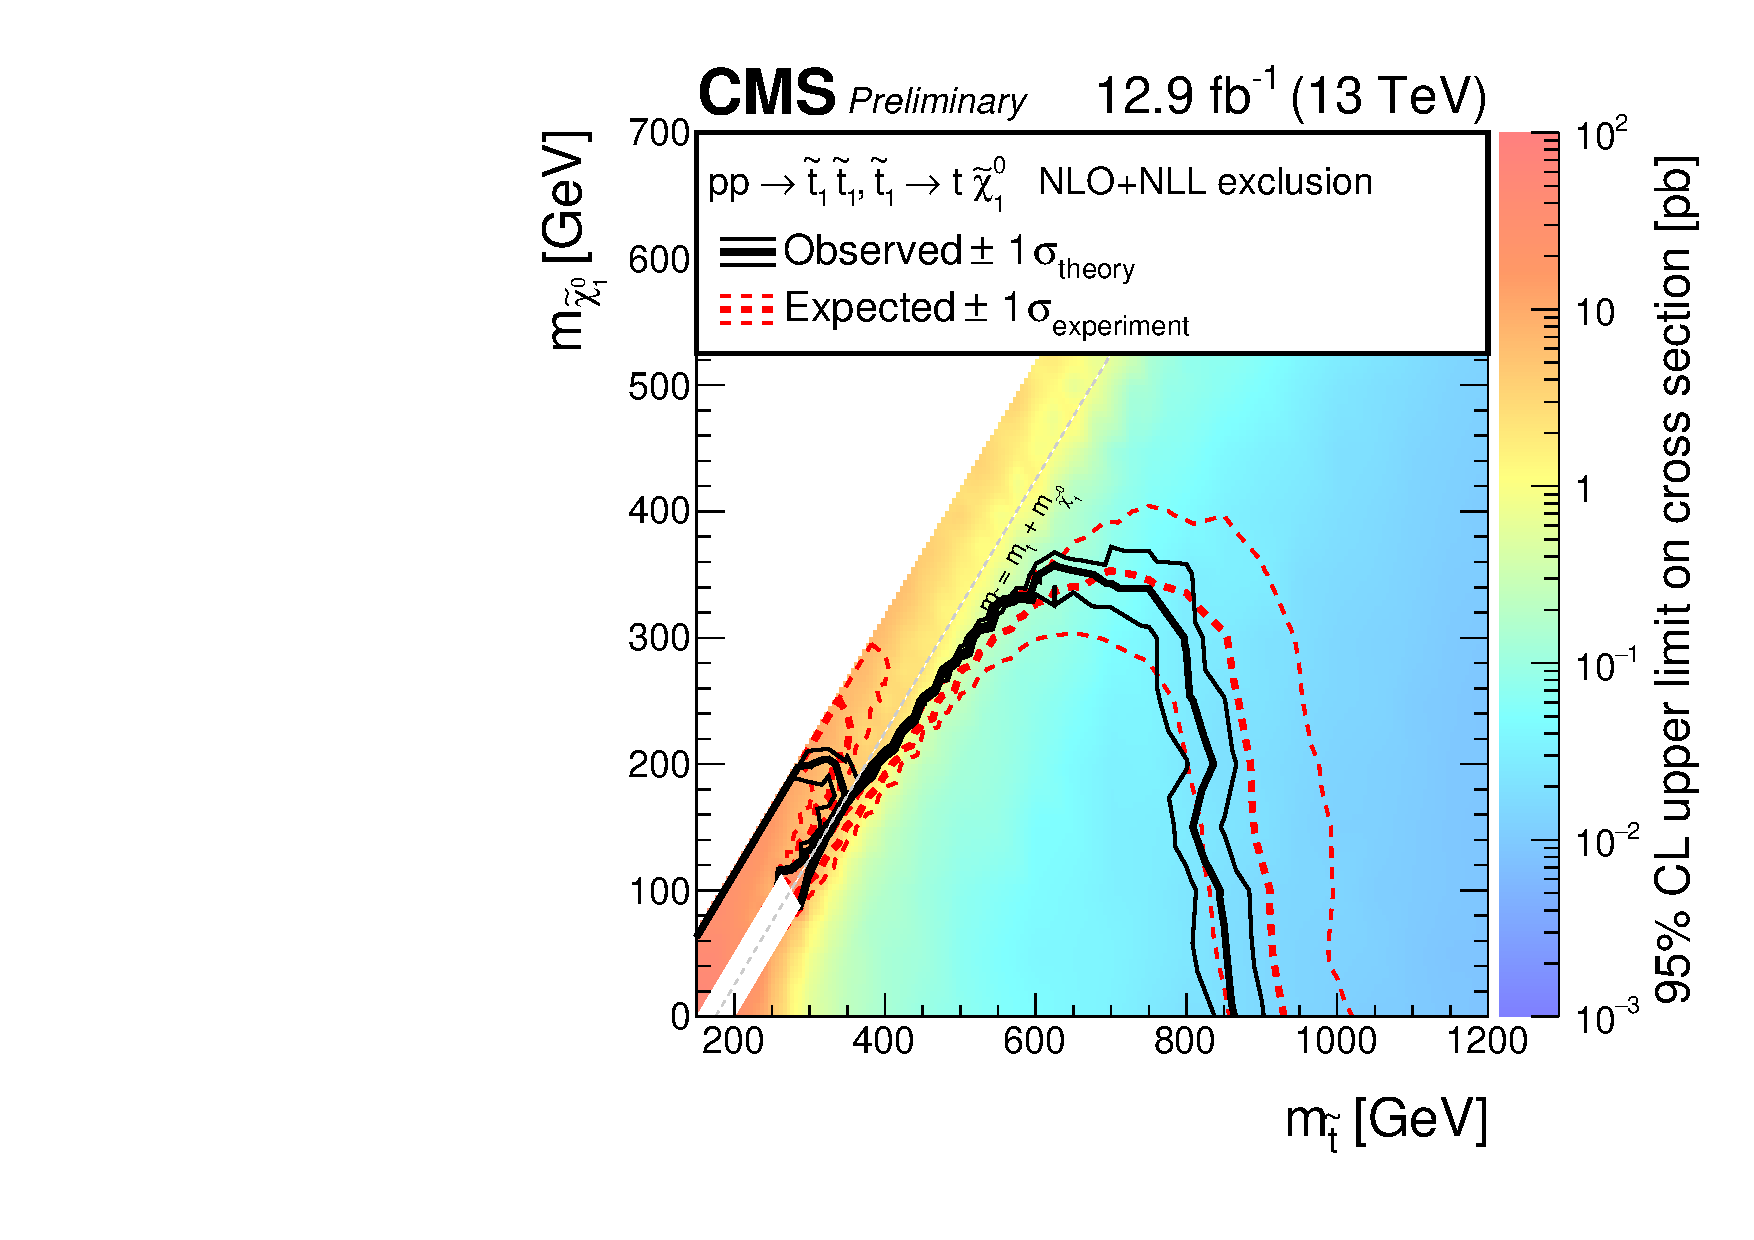
\includegraphics[width=0.6\textwidth]{figures/susyResults13/T2ttXSEC}
      \label{fig:T2tt_excl}
    } \\
    % \subfigure[T2tt: $\epsilon_{sig}^{\mathrm{4\,cat}}$]{
    %   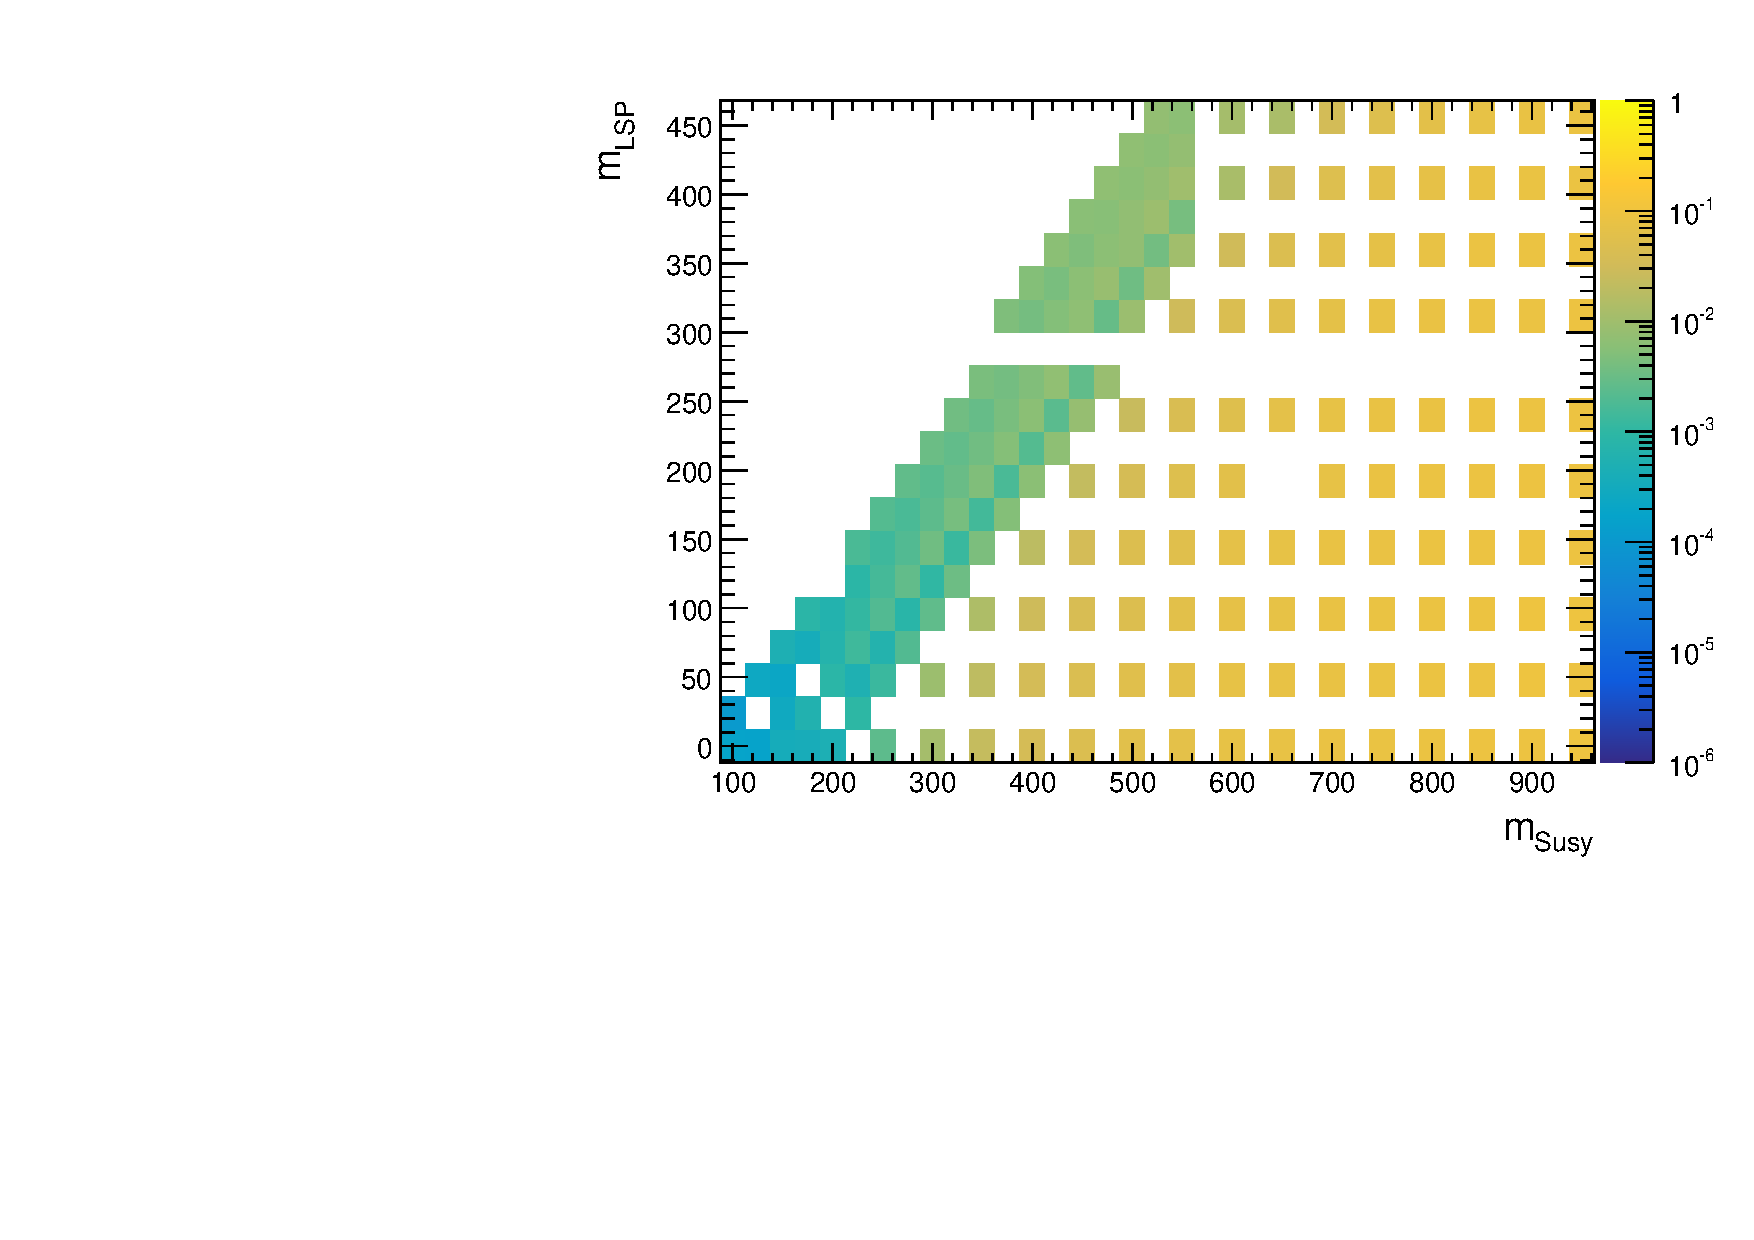
\includegraphics[width=0.45\textwidth]{figures/jetRanking/T2tt/eff/T2tt_merging_4_cats}
    %   \label{fig:T2tt_eff}
    % } ~~
    % \subfigure[T2tt: $\epsilon_{sig}^{\mathrm{4\,cat}}/\epsilon_{sig}^{\mathrm{tot}}$]{
    %   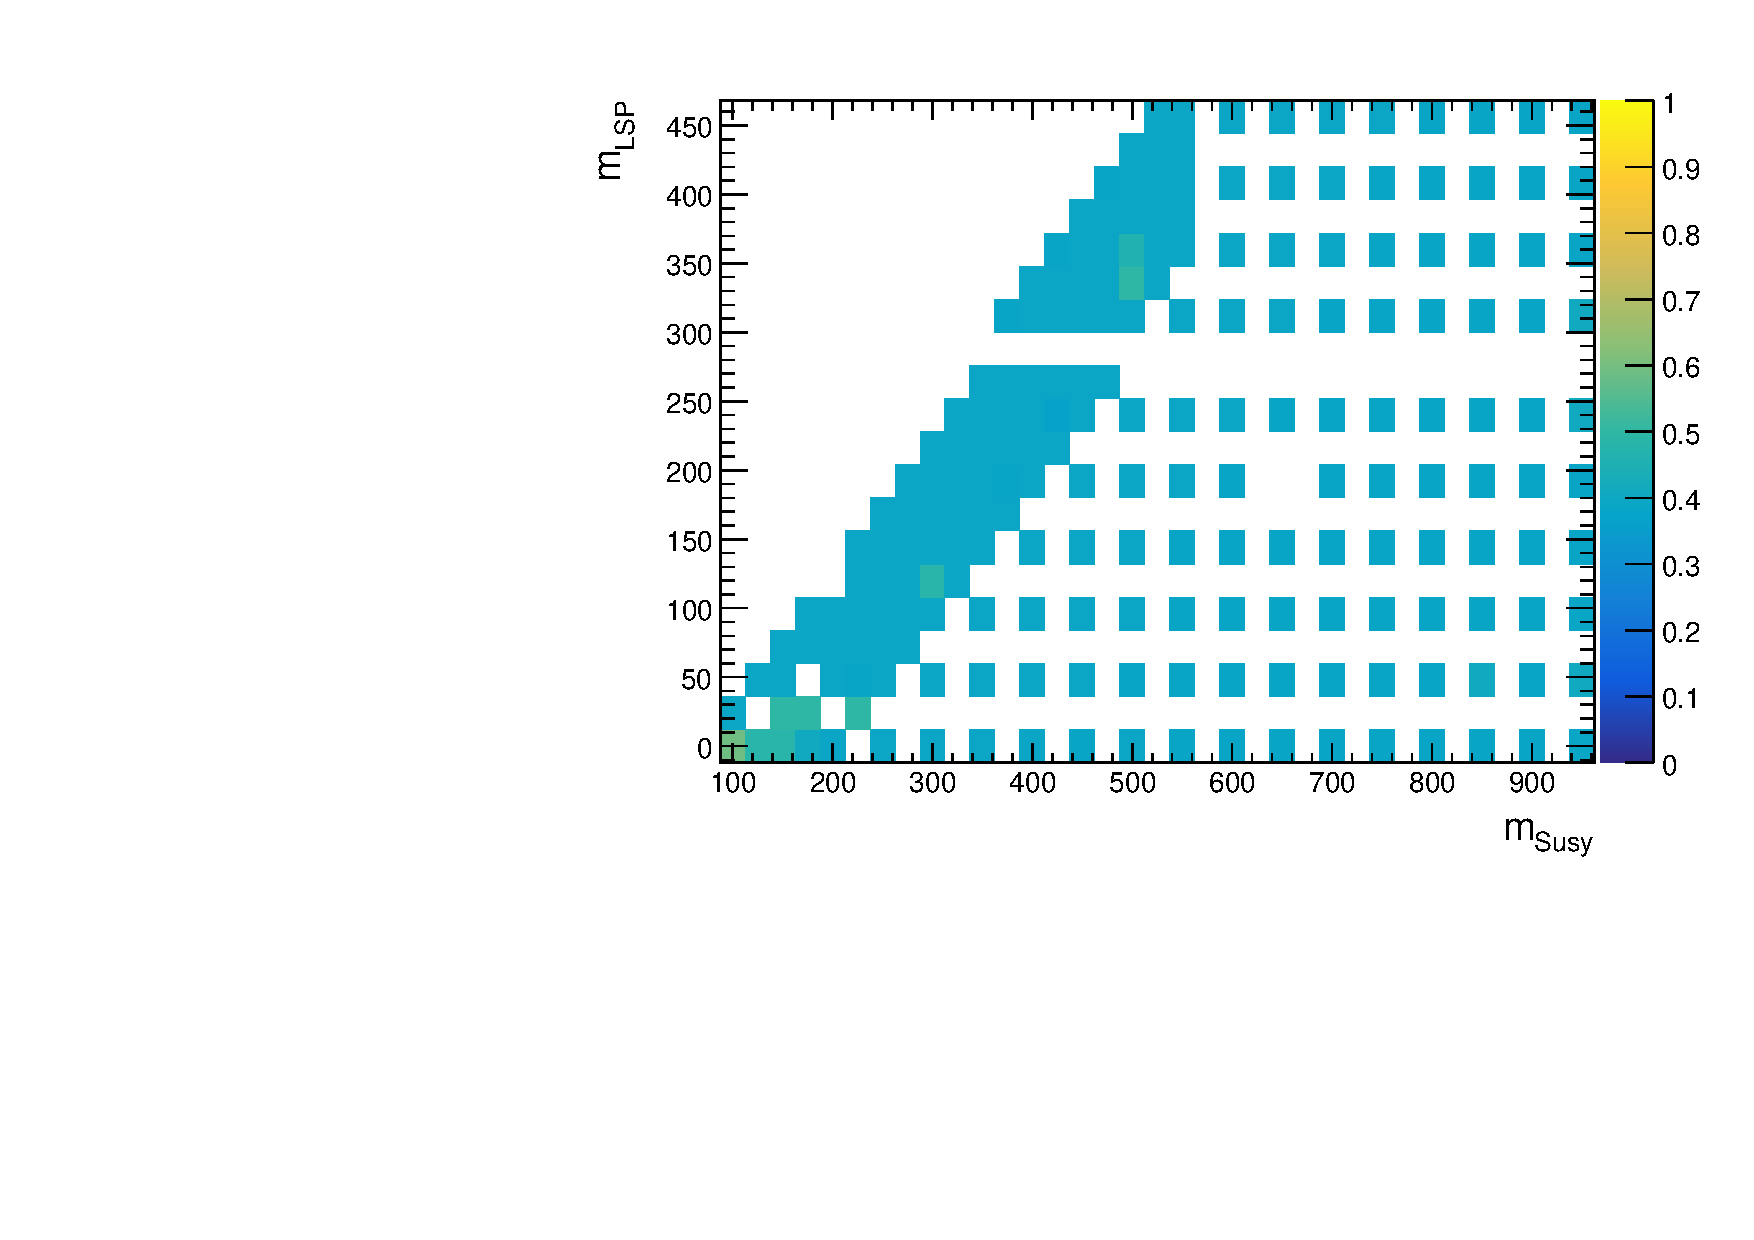
\includegraphics[width=0.45\textwidth]{figures/susyResults/T2tt_doubleRatioAcceptance}
    %   \label{fig:T2tt_eff_doubleRatio}
    % }
    \caption{
      The 95\% C.L. observed upper limit on the cross section (histogram), with the expected (solid black line) observed (solid red line) exclusion contours. 
      % Bottom left: signal acceptance including the 4 most excluding jet categories. 
      % Bottom right: ratio of the signal acceptance including 4 categories to the acceptance including the whole signal region. 
    }
    \label{fig:T2tt}
  \end{center}
\end{figure}
\newpage
\begin{figure}[h!]
  \begin{center}
    \subfigure[T2bb: Upper limit on the cross section in the $(m_{\mathrm{Gluino}},m_{\mathrm{Susy}})$ plane]{
      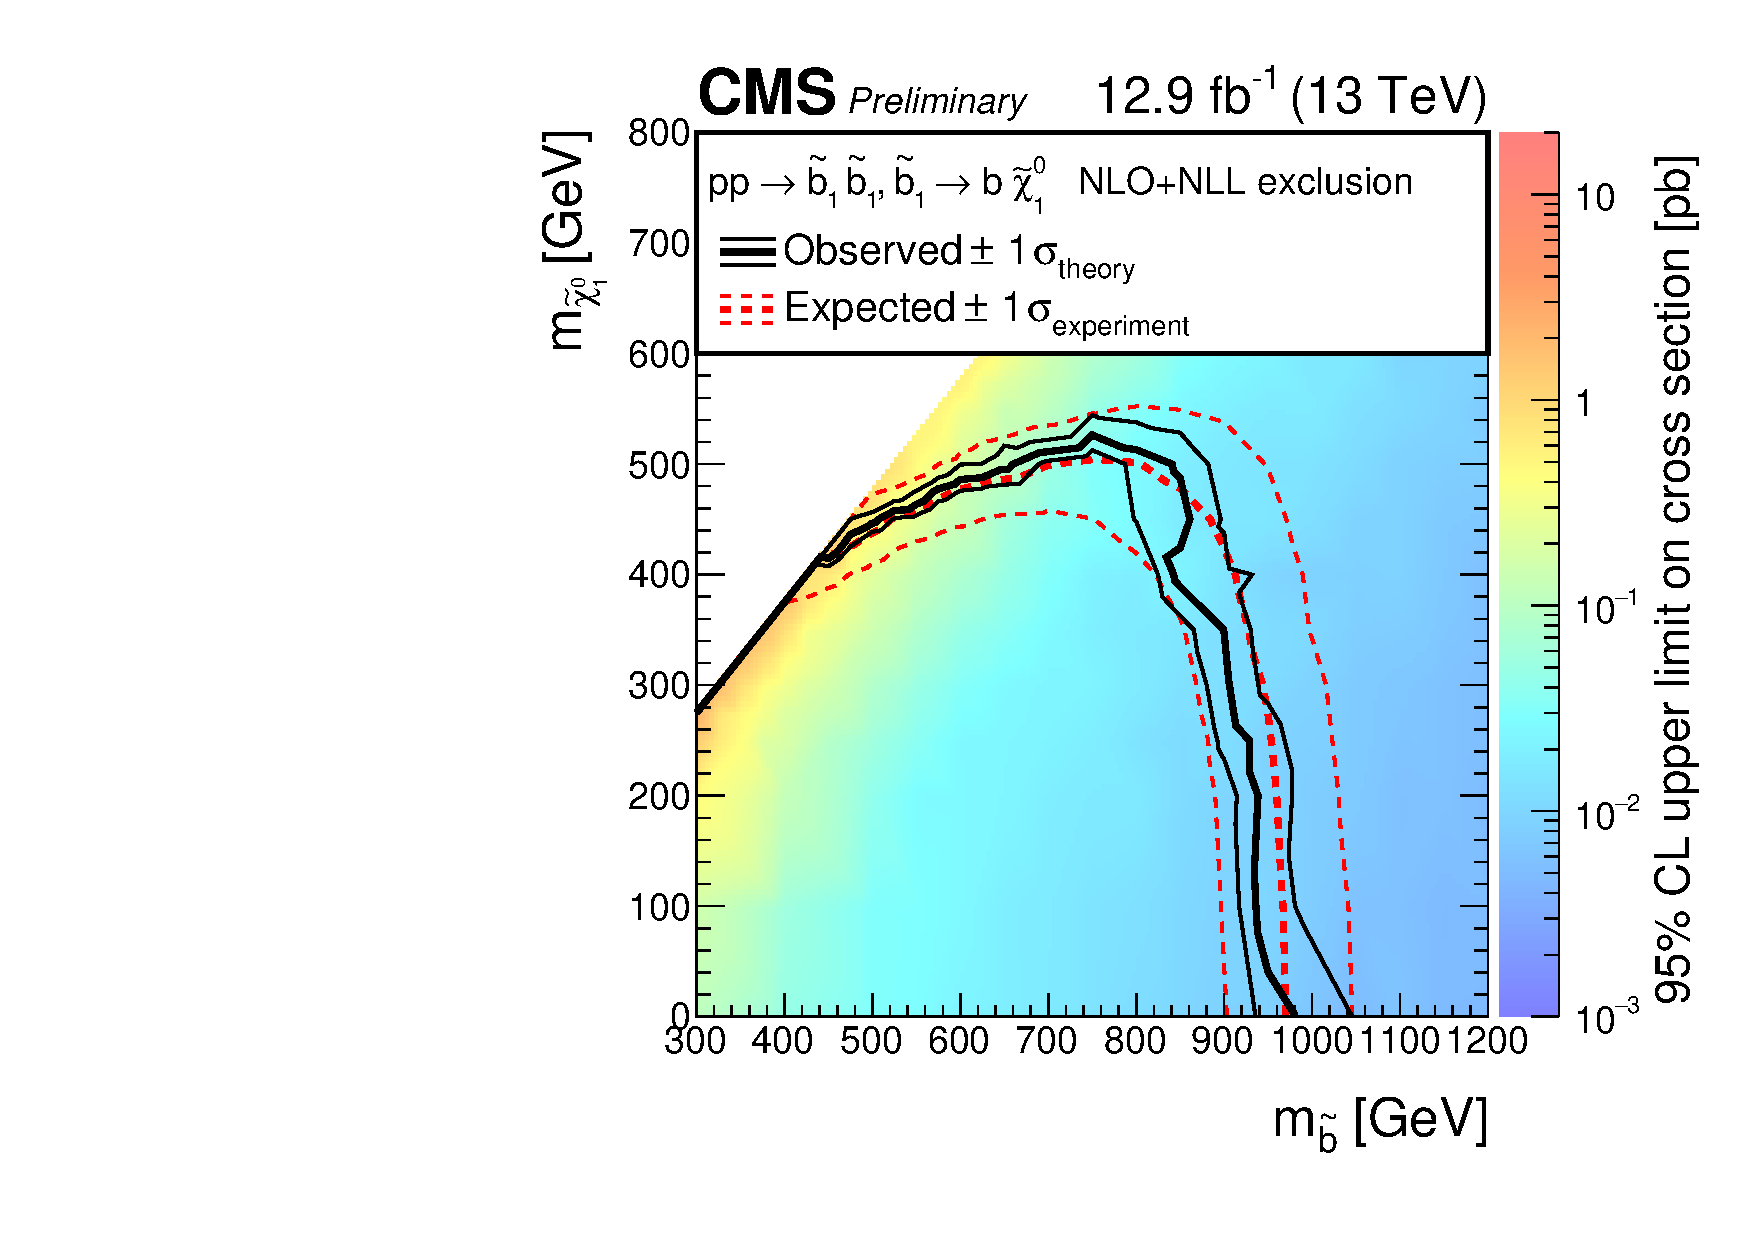
\includegraphics[width=0.6\textwidth]{figures/susyResults13/T2bbXSEC}
      \label{fig:T2bb_excl}
    } \\
    % \subfigure[T2bb: $\epsilon_{sig}^{\mathrm{4\,cat}}$]{
    %   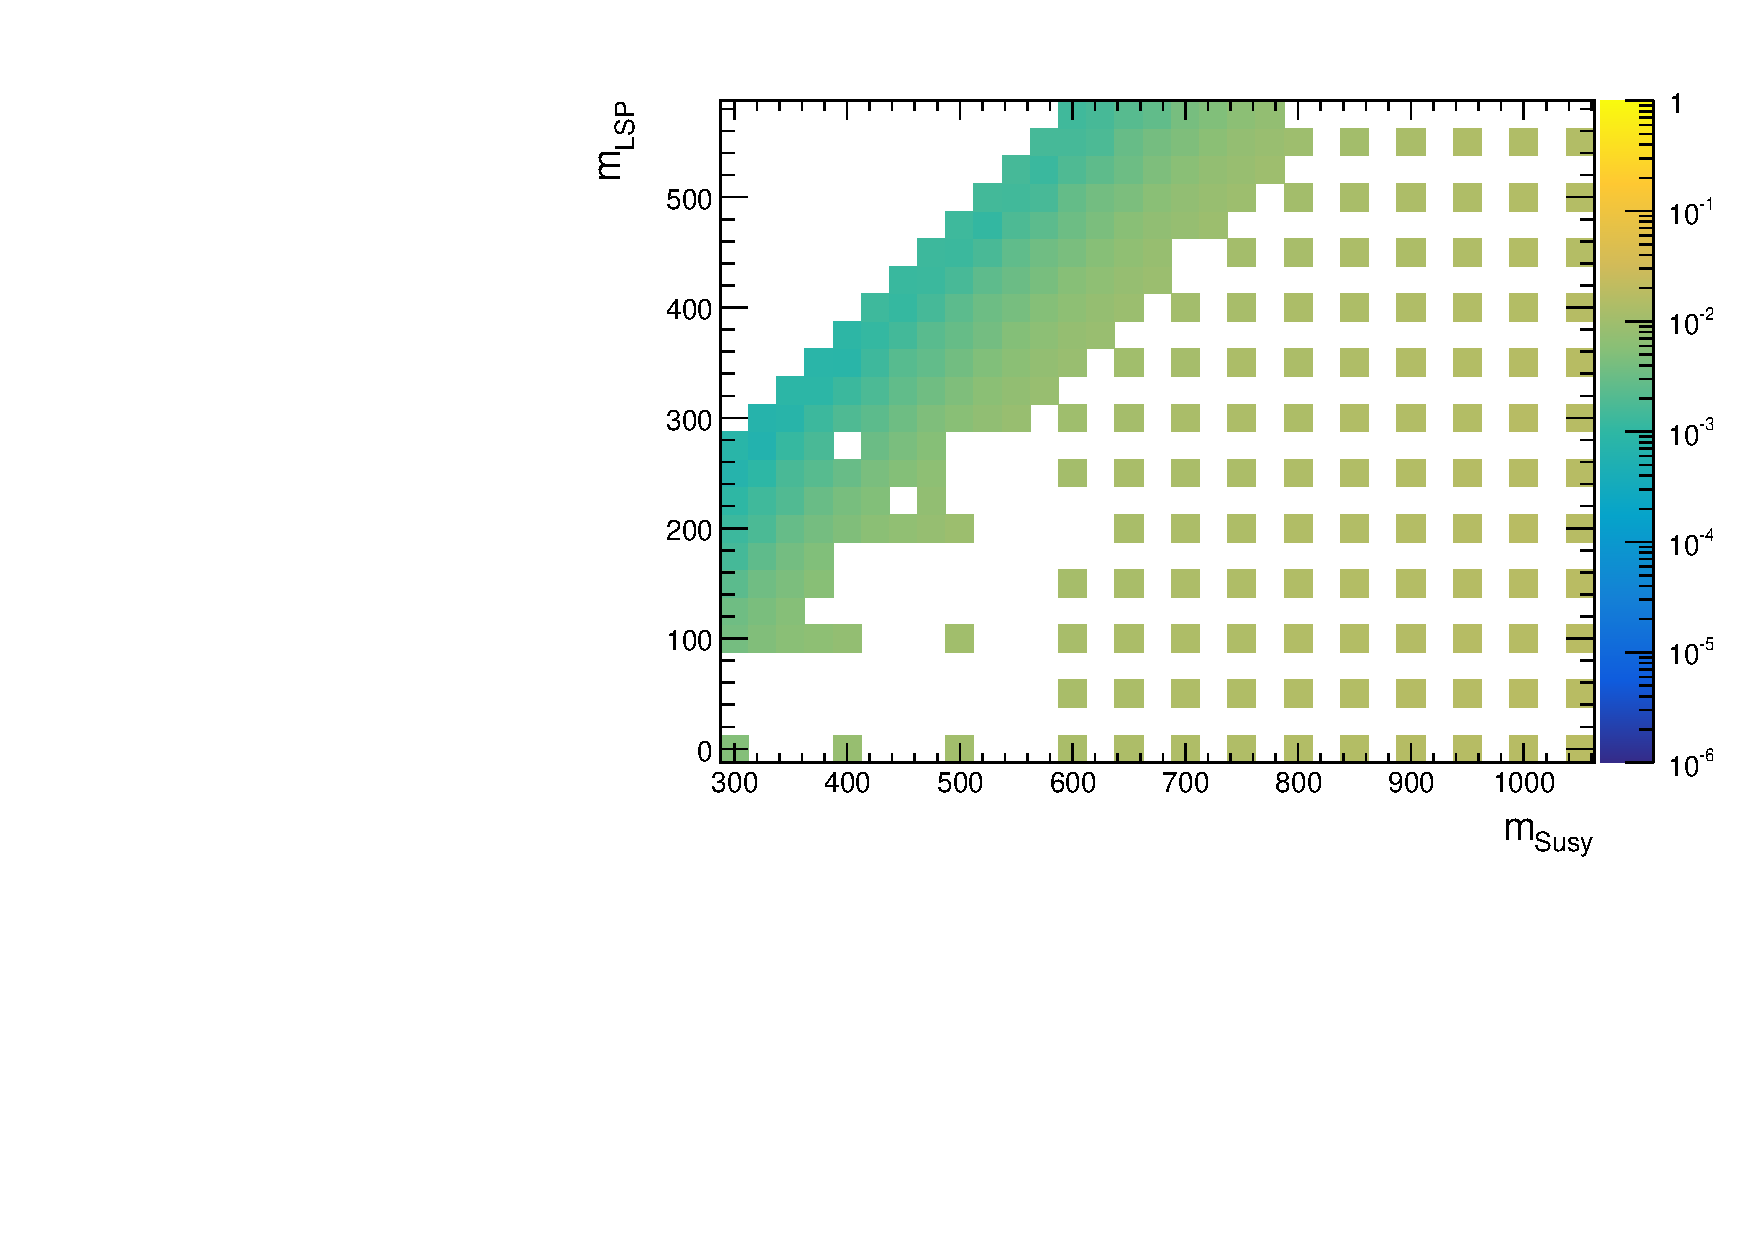
\includegraphics[width=0.45\textwidth]{figures/jetRanking/T2bb/eff/T2bb_merging_4_cats}
    %   \label{fig:T2bb_eff}
    % } ~~
    % \subfigure[T2bb: $\epsilon_{sig}^{\mathrm{4\,cat}}/\epsilon_{sig}^{\mathrm{tot}}$]{
    %   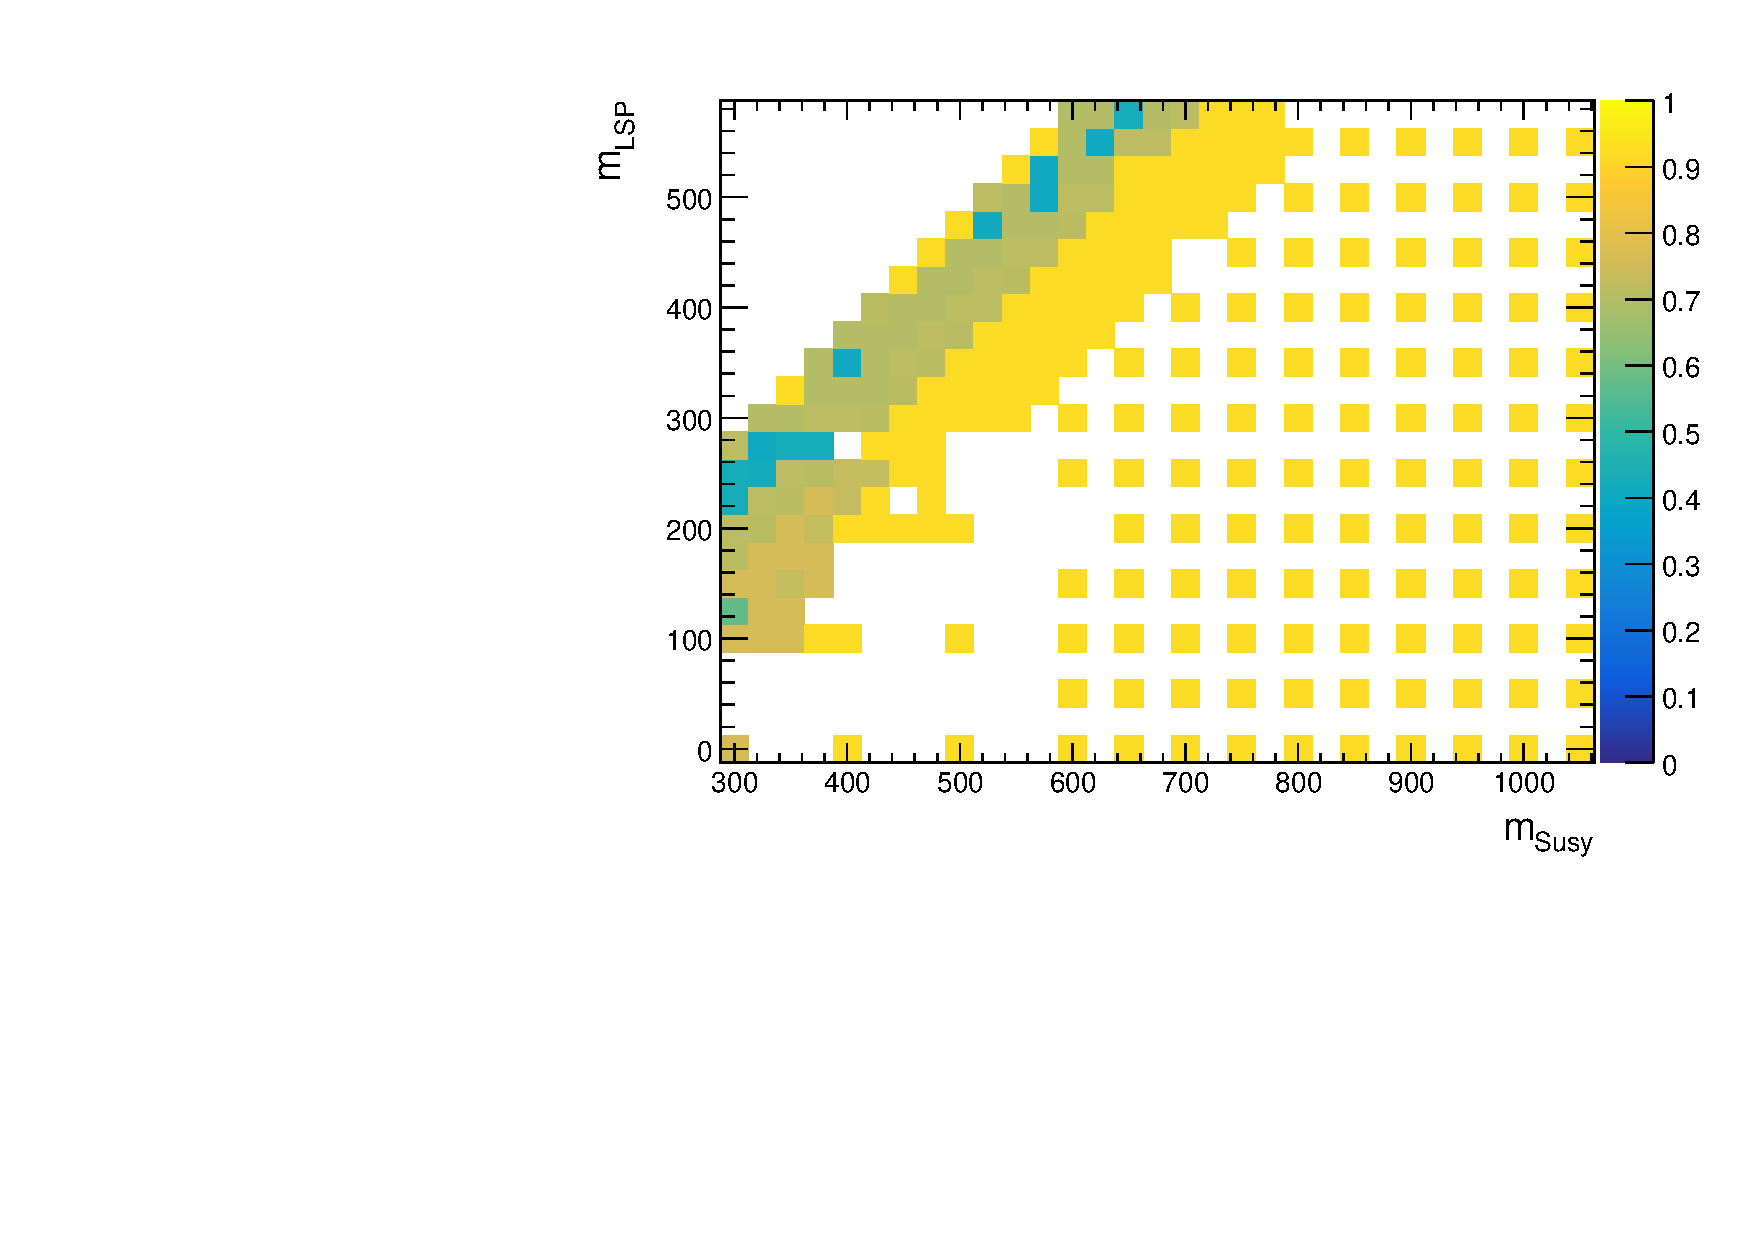
\includegraphics[width=0.45\textwidth]{figures/susyResults/T2bb_doubleRatioAcceptance}
    %   \label{fig:T2bb_eff_doubleRatio}
    % }
    \caption{
      The 95\% C.L. observed upper limit on the cross section (histogram), with the expected (solid black line) observed (solid red line) exclusion contours. 
      % Bottom left: signal acceptance including the 4 most excluding jet categories. 
      % Bottom right: ratio of the signal acceptance including 4 categories to the acceptance including the whole signal region. 
    }
    \label{fig:T2bb}
  \end{center}
\end{figure}
\newpage

\begin{figure}[h!]
  \begin{center}
    \subfigure[T2qq: Upper limit on the cross section in the $(m_{\mathrm{Gluino}},m_{\mathrm{Susy}})$ plane]{
      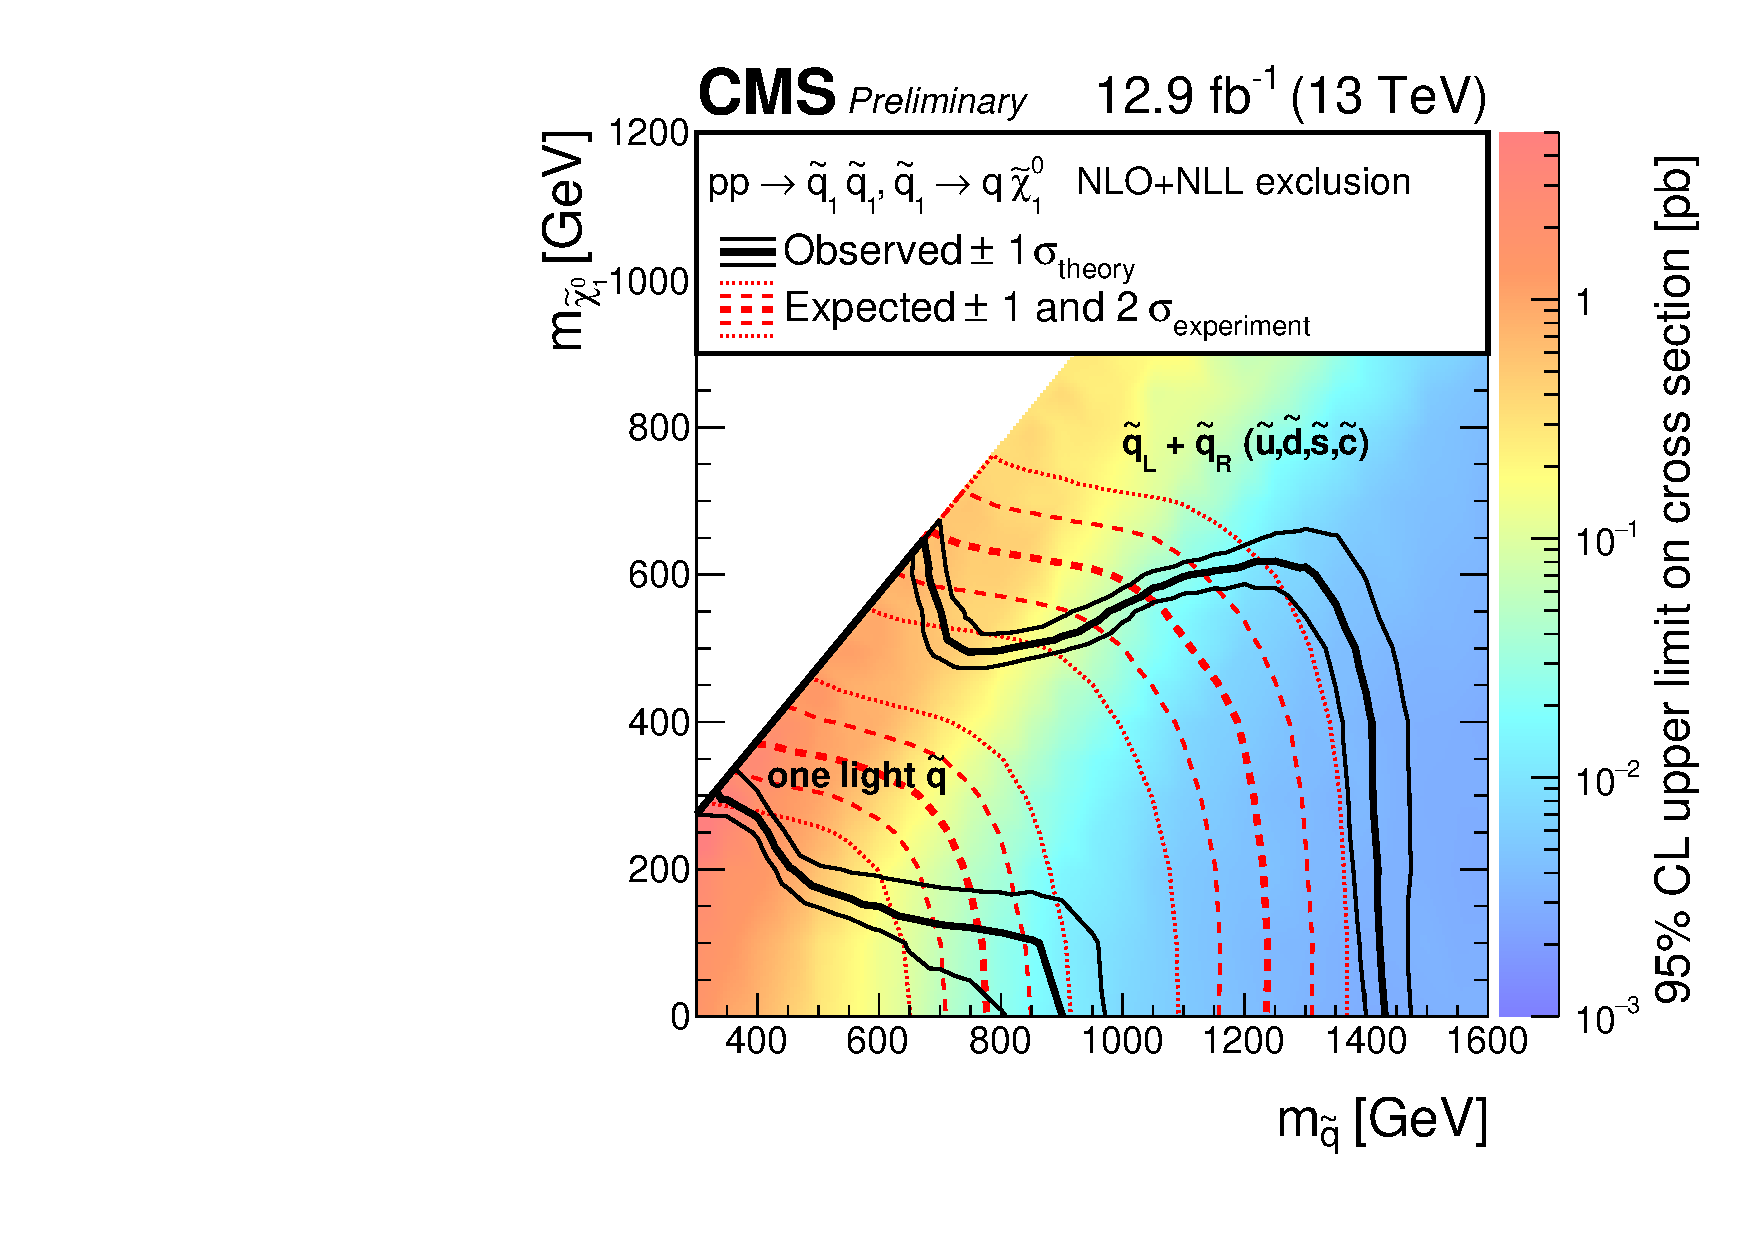
\includegraphics[width=0.6\textwidth]{figures/susyResults13/T2qqXSEC}
      \label{fig:T2qq_excl}
    } \\
    % \subfigure[T2qq: $\epsilon_{sig}^{\mathrm{4\,cat}}$]{
    %   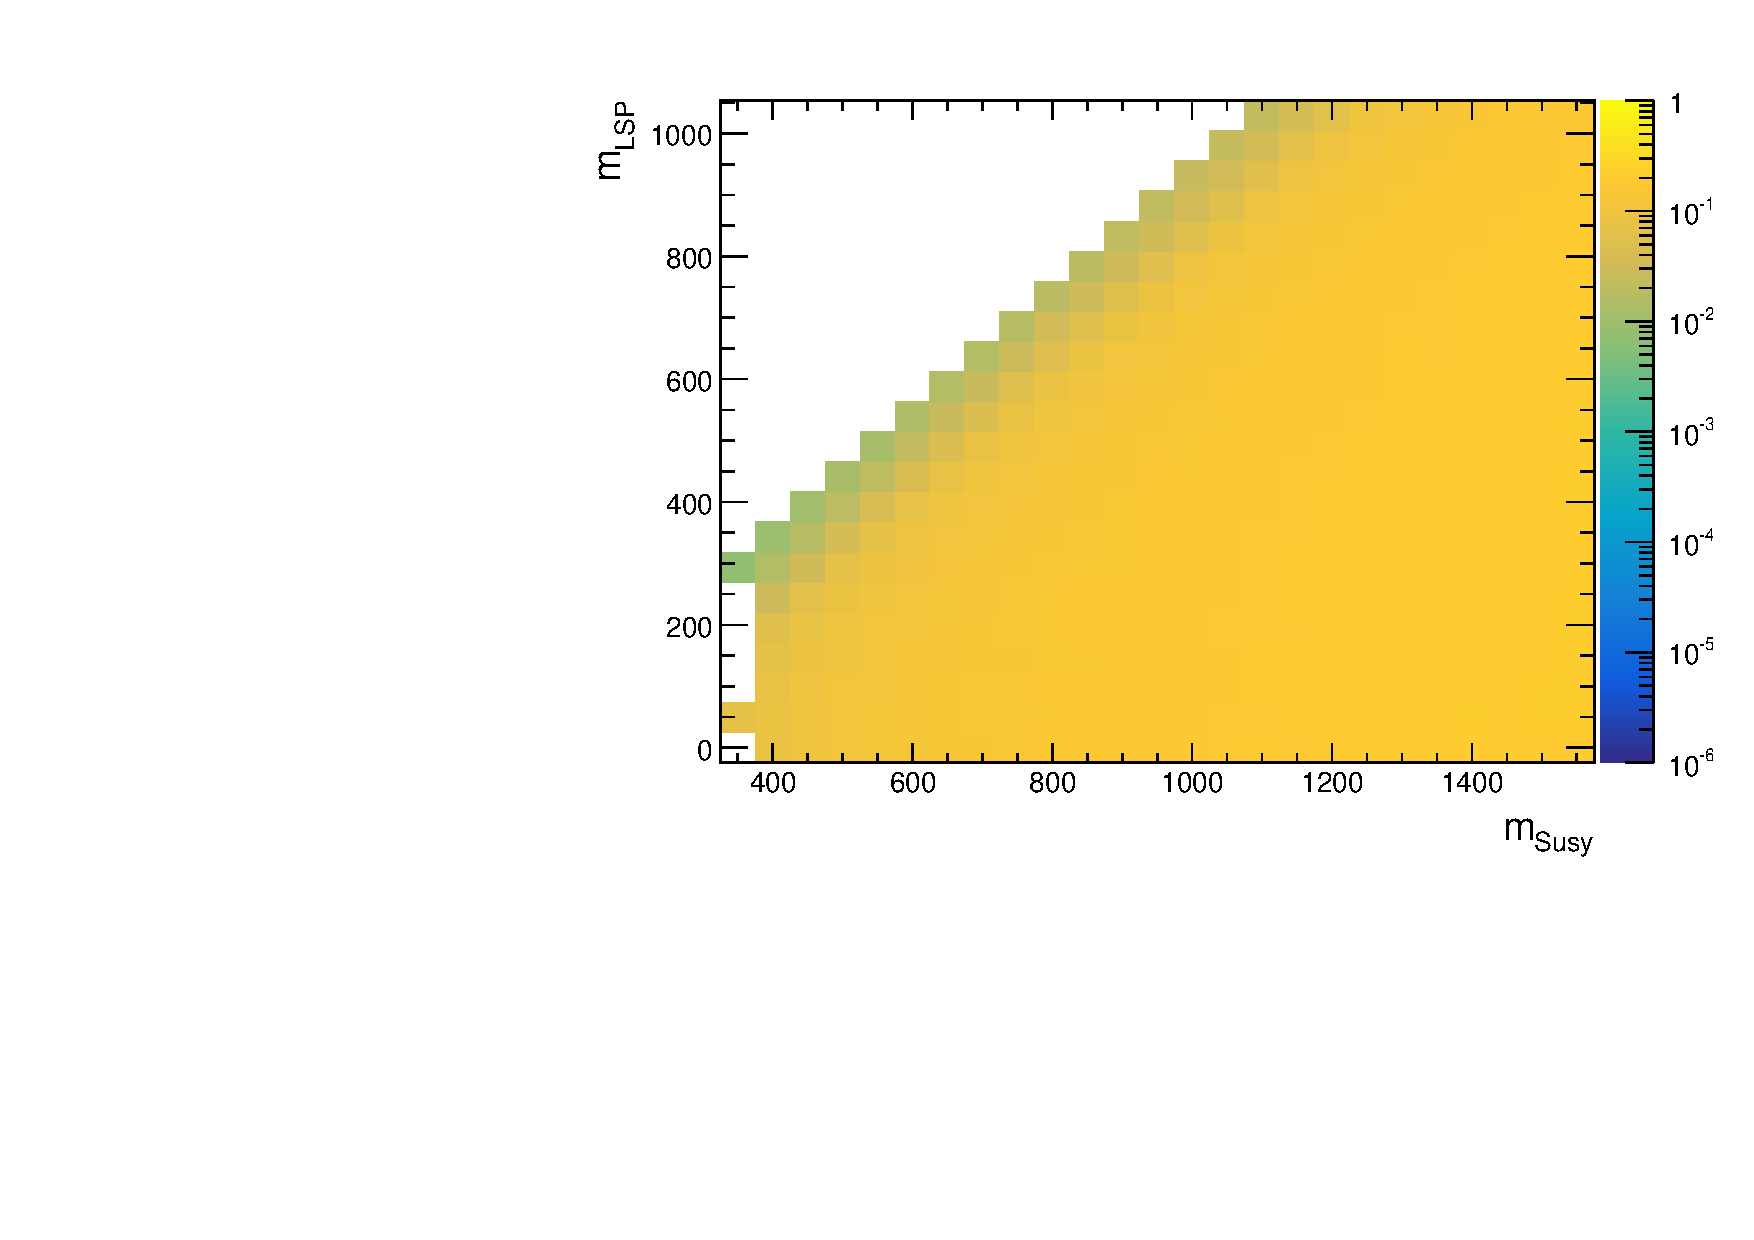
\includegraphics[width=0.45\textwidth]{figures/jetRanking/T2qq/eff/T2qq_merging_4_cats}
    %   \label{fig:T2qq_eff}
    % } ~~
    % \subfigure[T2qq: $\epsilon_{sig}^{\mathrm{4\,cat}}/\epsilon_{sig}^{\mathrm{tot}}$]{
    %   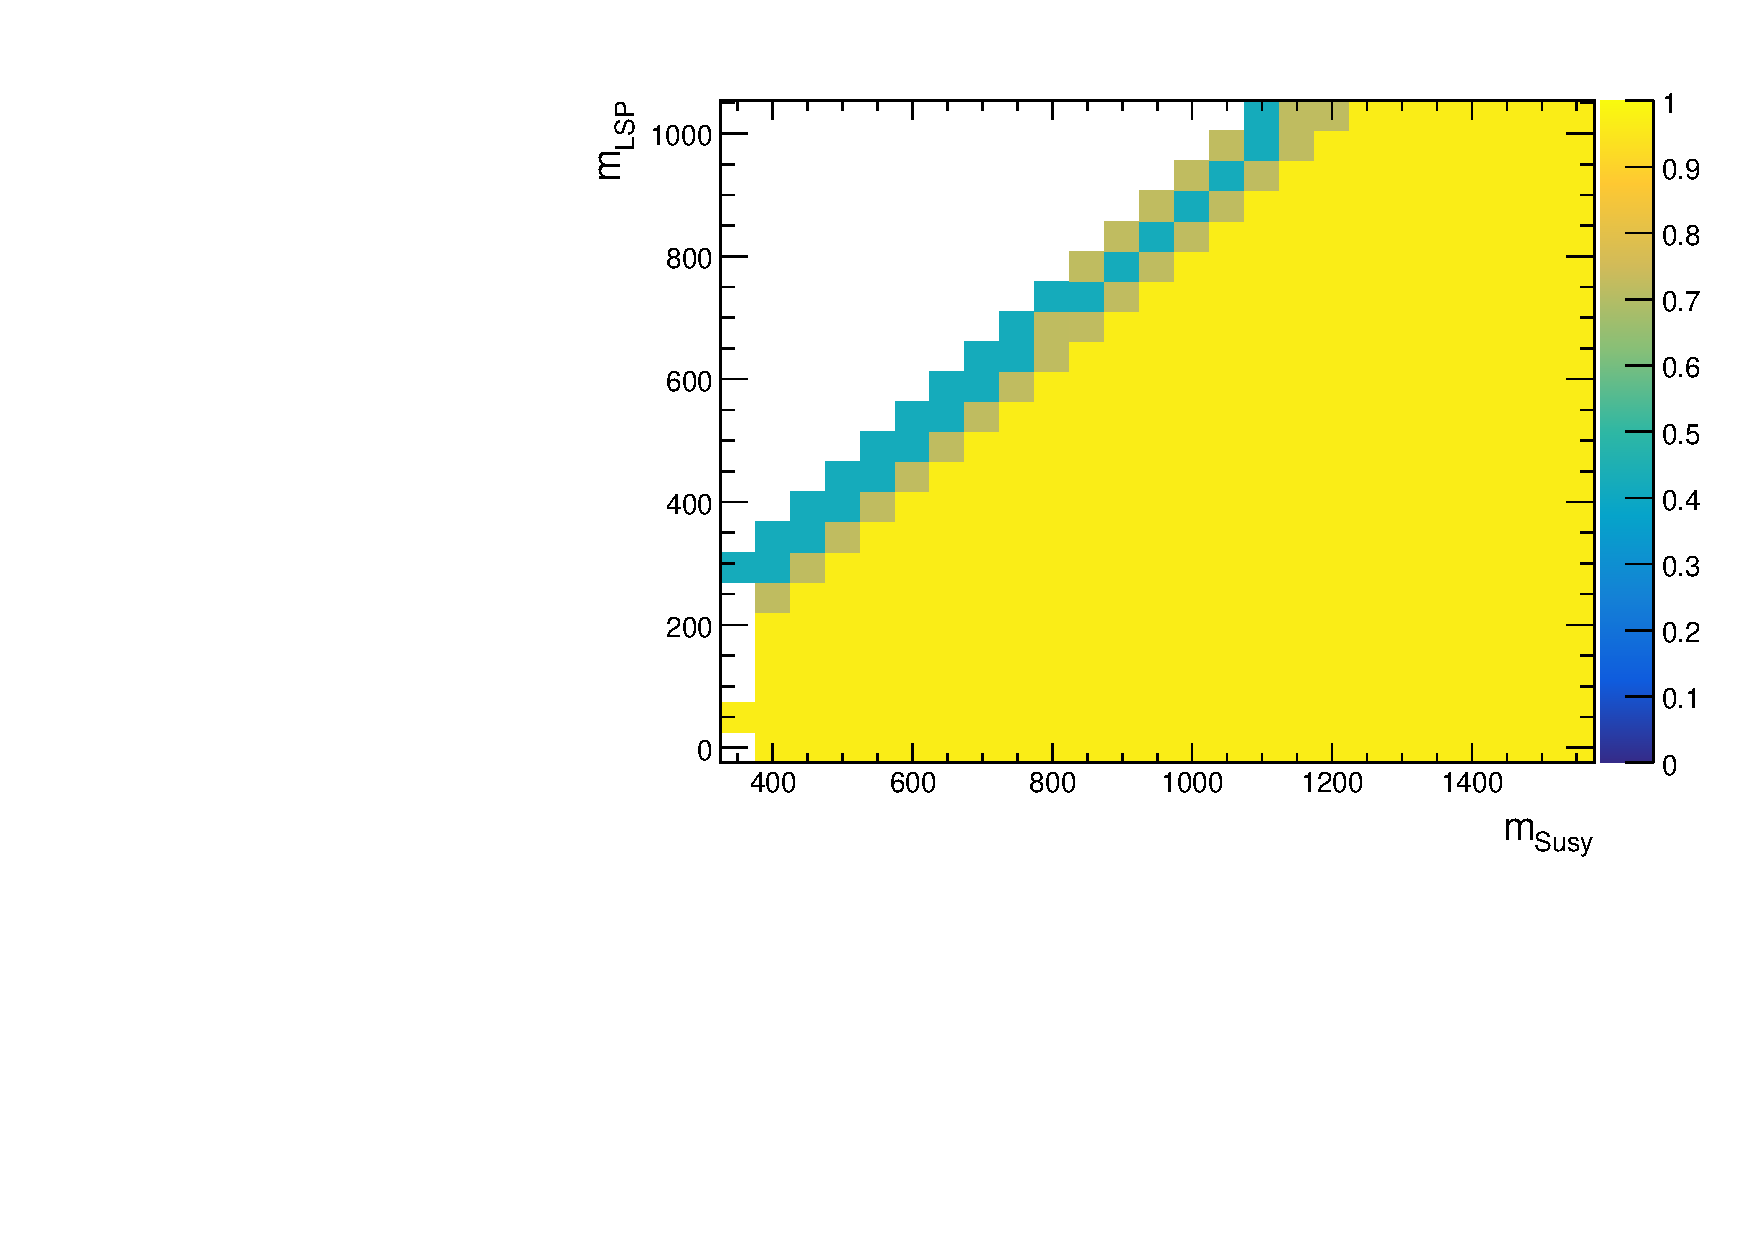
\includegraphics[width=0.45\textwidth]{figures/susyResults/T2qq_doubleRatioAcceptance}
    %   \label{fig:T2qq_eff_doubleRatio}
    % }
    \caption{
      The 95\% C.L. observed upper limit on the cross section (histogram), with the expected (solid black line) observed (solid red line) exclusion contours. 
      % Bottom left: signal acceptance including the 4 most excluding jet categories. 
      % Bottom right: ratio of the signal acceptance including 4 categories to the acceptance including the whole signal region. 
    }
    \label{fig:T2qq}
  \end{center}
\end{figure}

\newpage
\begin{figure}[h!]
  \begin{center}
    \subfigure[T1tttt: Upper limit on the cross section in the $(m_{\mathrm{Gluino}},m_{\mathrm{Susy}})$ plane]{
      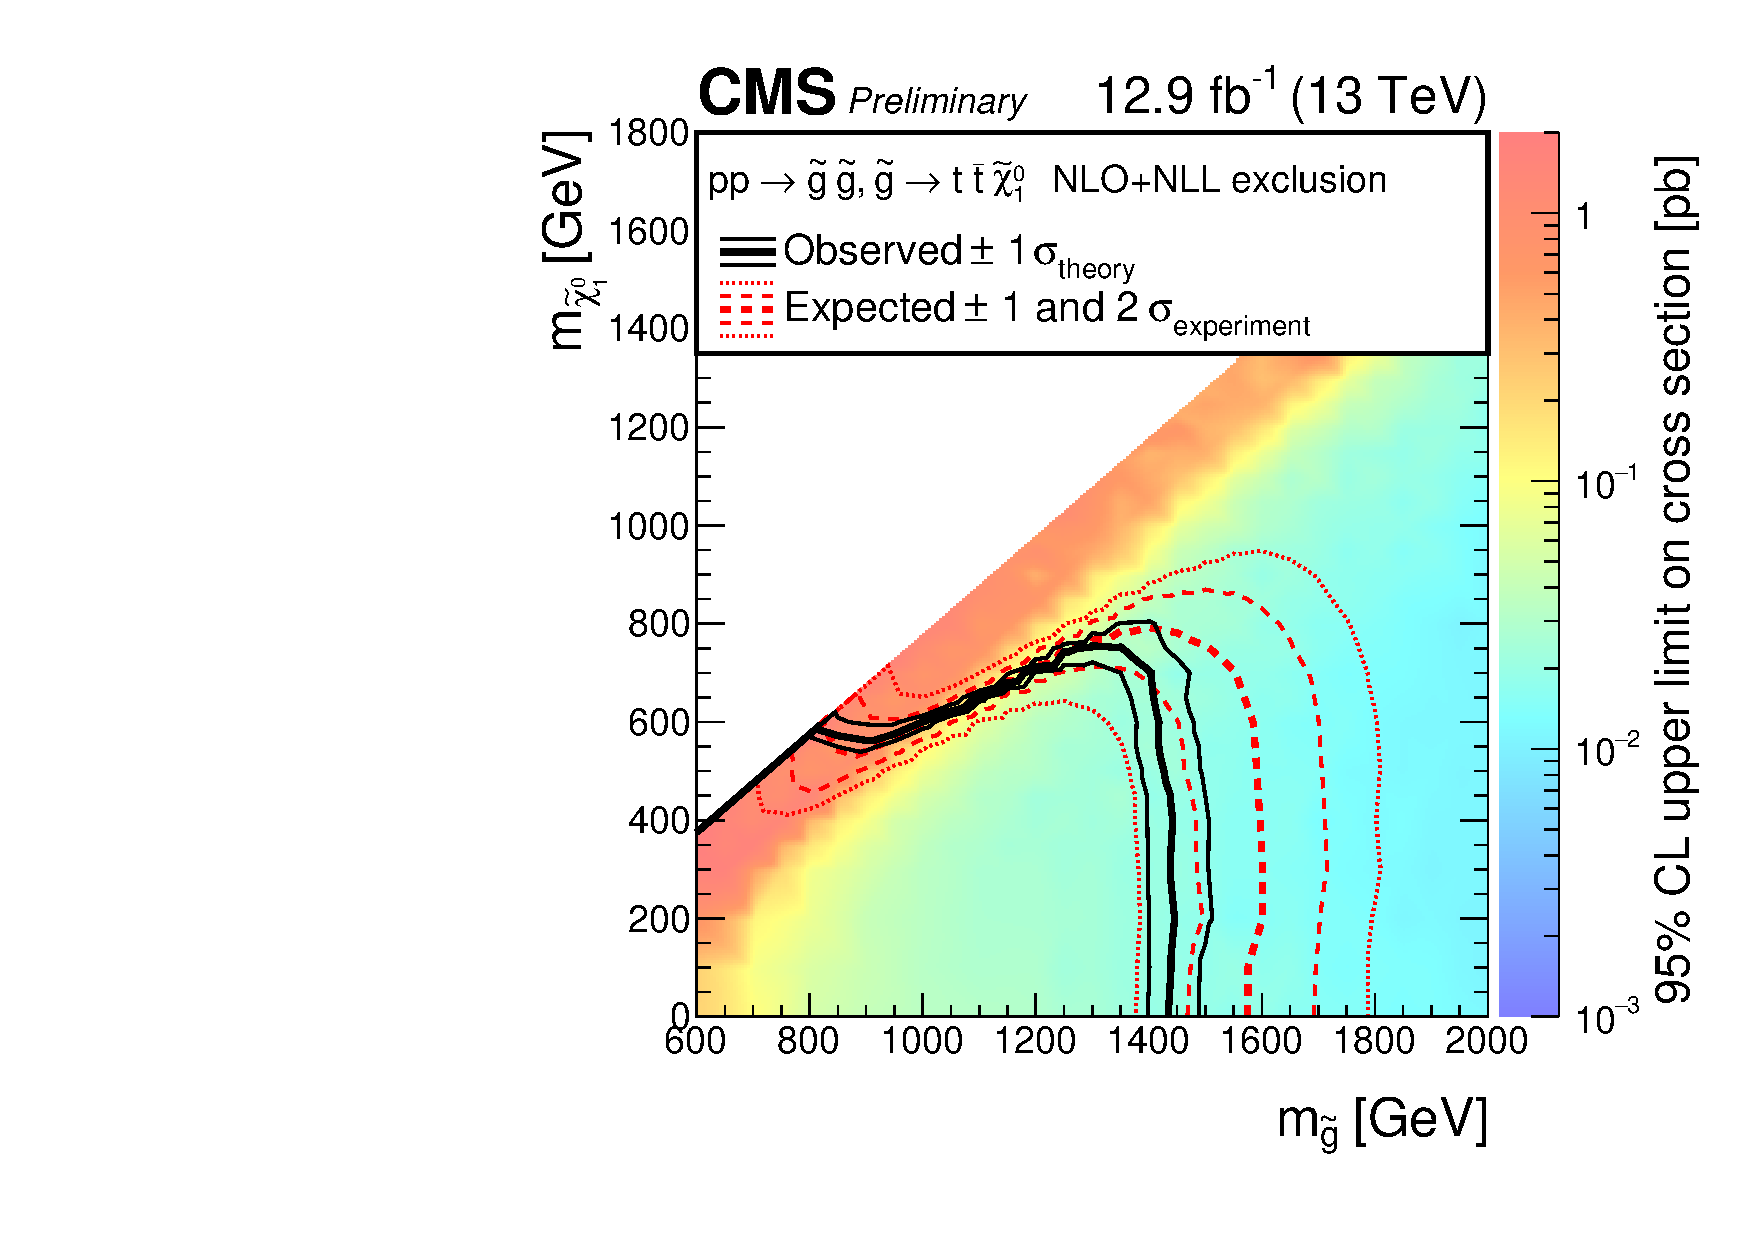
\includegraphics[width=0.6\textwidth]{figures/susyResults13/T1ttttXSEC}
      \label{fig:T1tttt_excl}
    } \\
    % \subfigure[T1tttt: $\epsilon_{sig}^{\mathrm{4\,cat}}$]{
    %   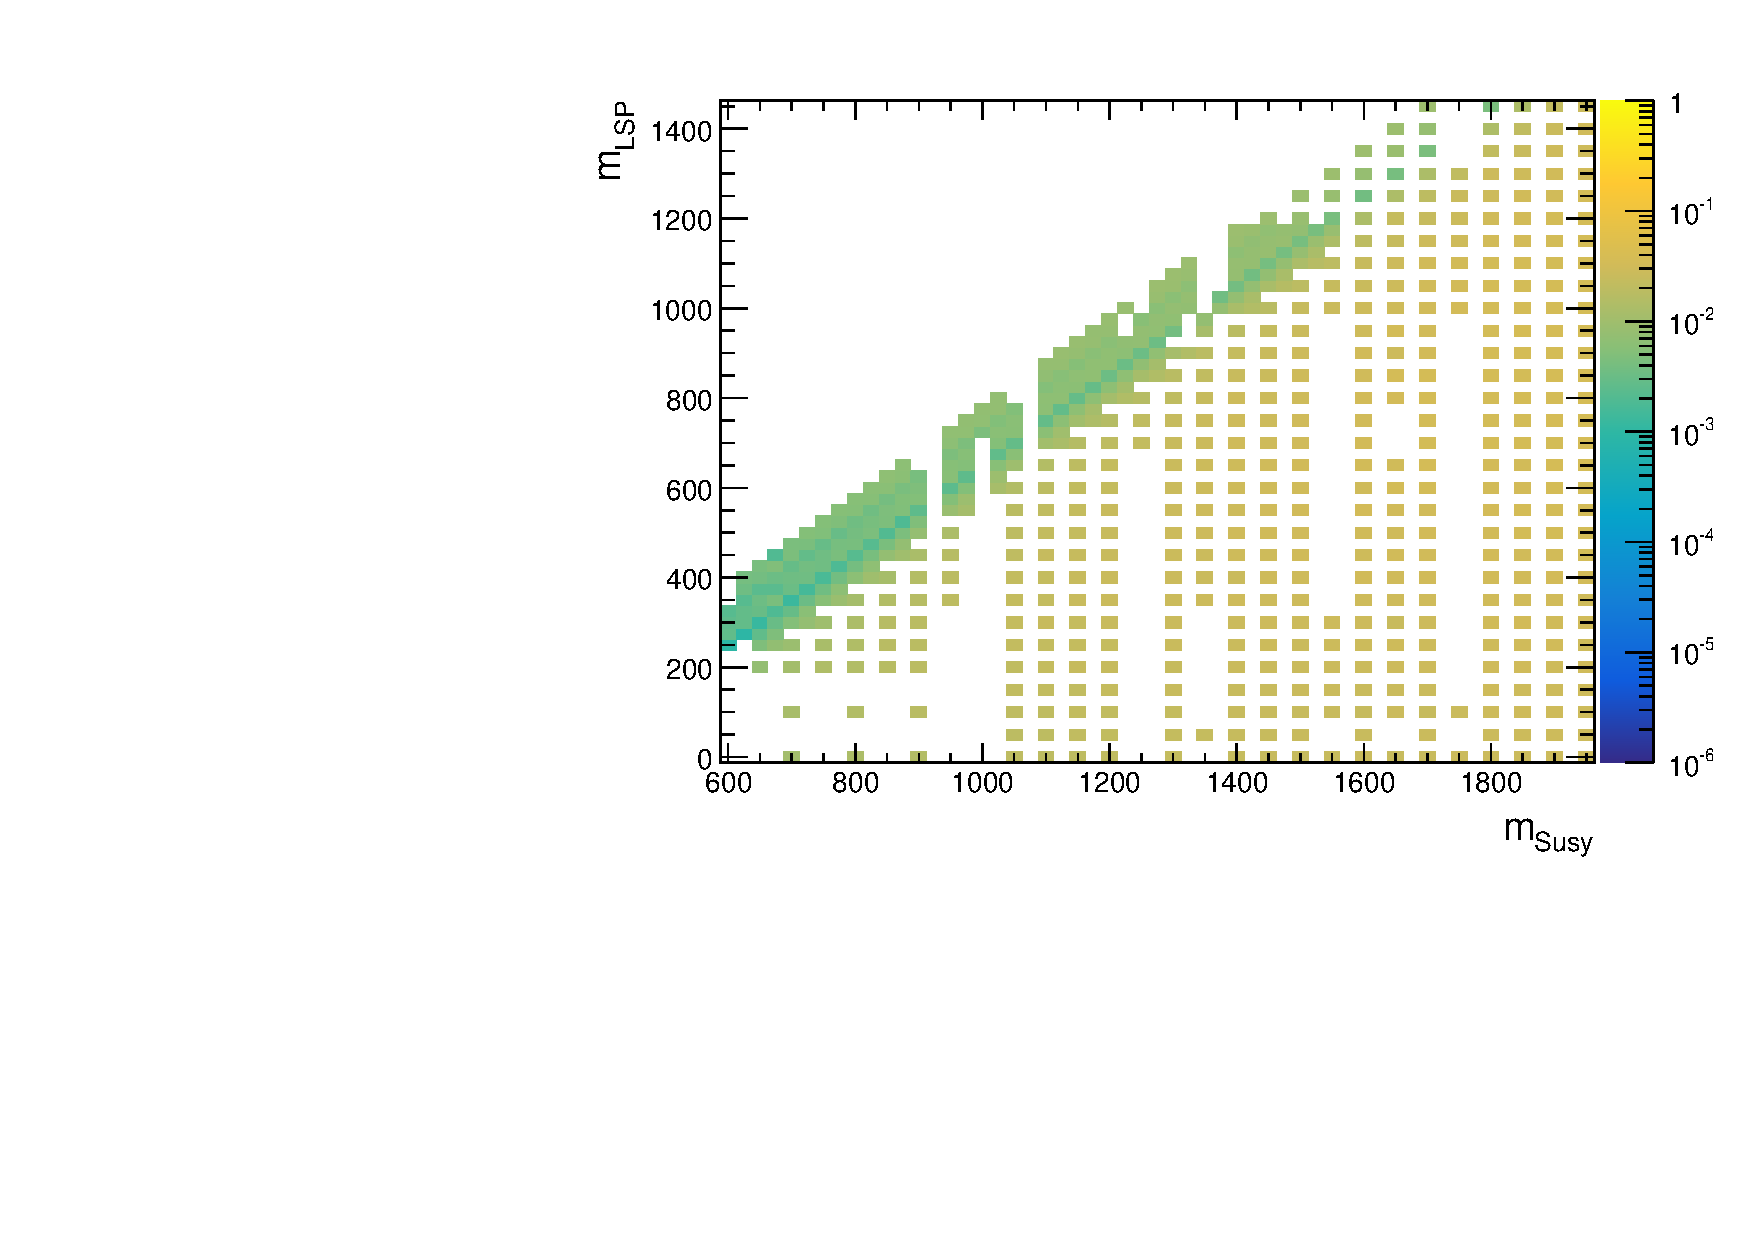
\includegraphics[width=0.45\textwidth]{figures/jetRanking/T1tttt/eff/T1tttt_merging_4_cats}
    %   \label{fig:T1tttt_eff}
    % } ~~
    % \subfigure[T1tttt: $\epsilon_{sig}^{\mathrm{4\,cat}}/\epsilon_{sig}^{\mathrm{tot}}$]{
    %   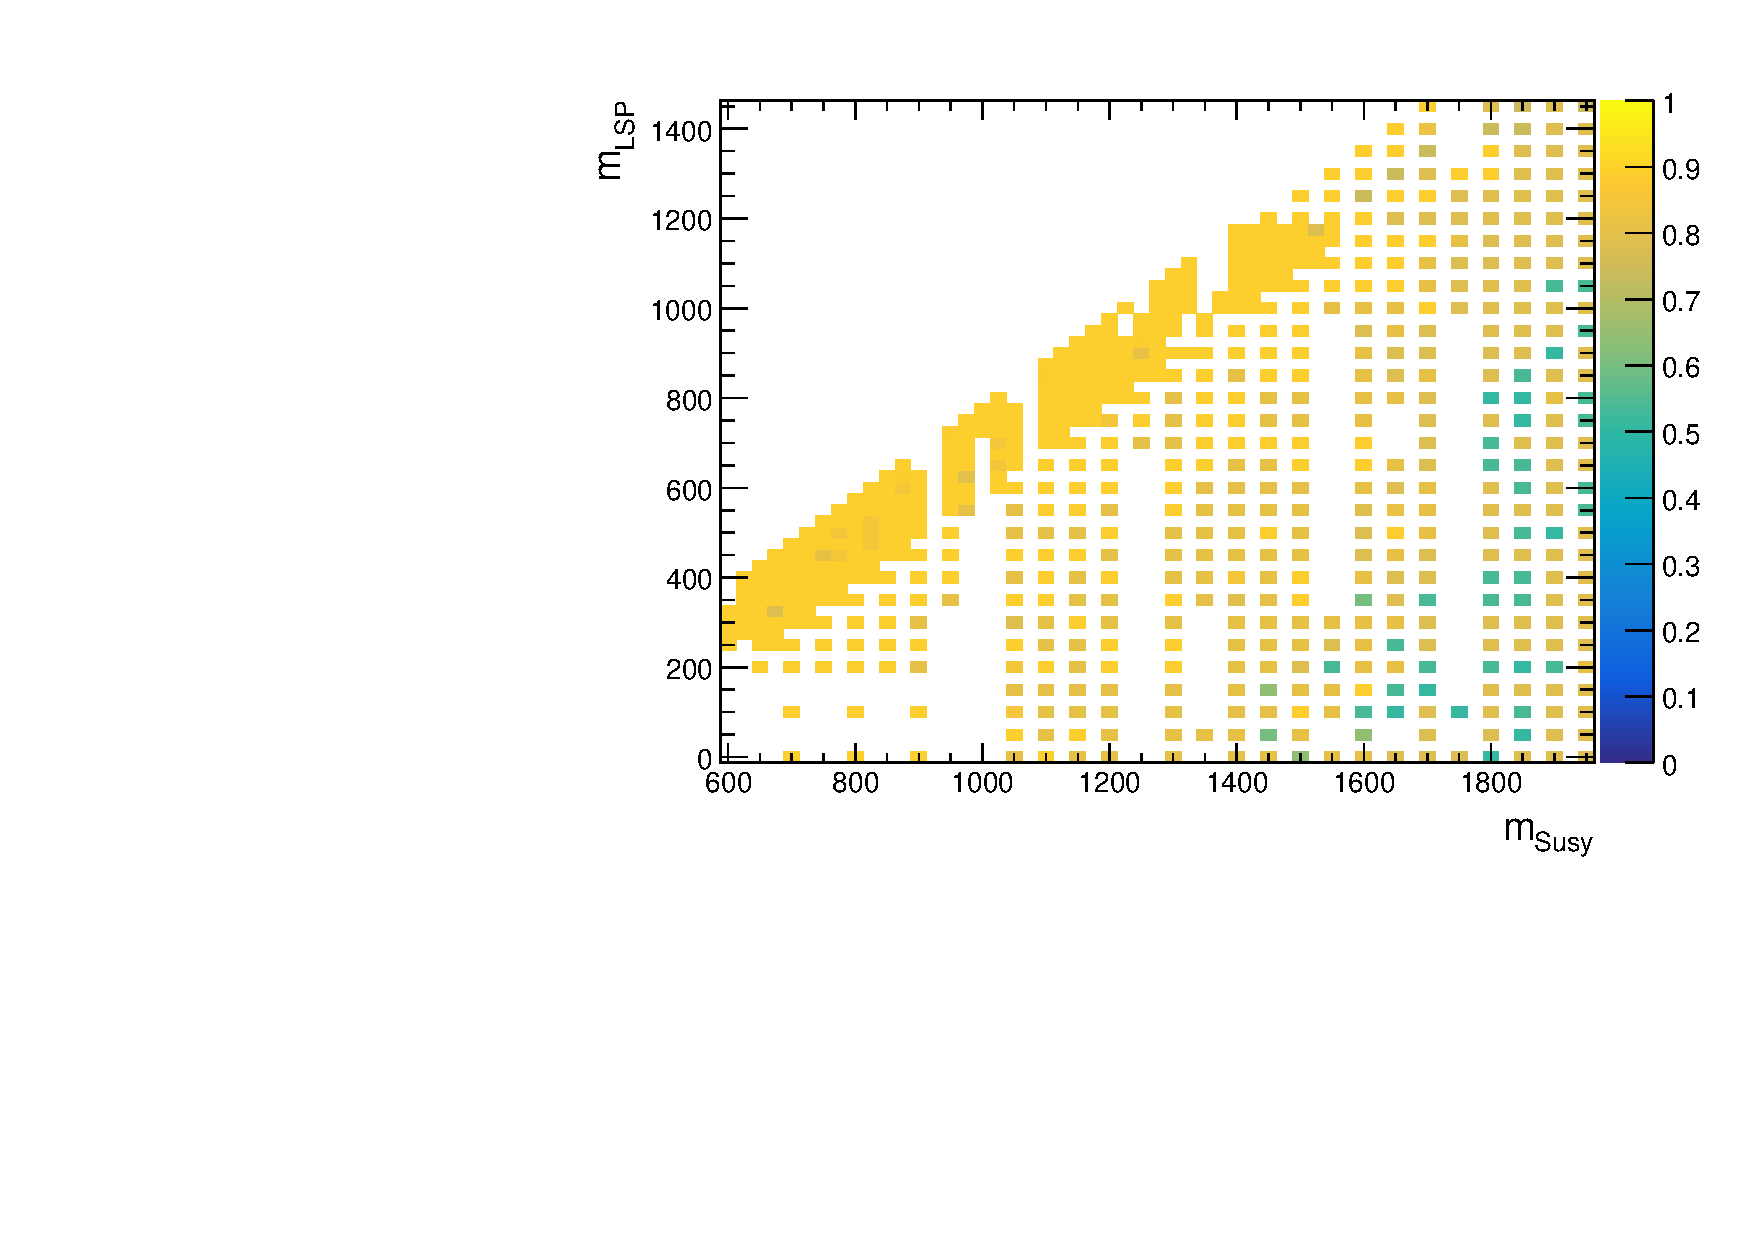
\includegraphics[width=0.45\textwidth]{figures/susyResults/T1tttt_doubleRatioAcceptance}
    %   \label{fig:T1tttt_eff_doubleRatio}
    % }
    \caption{
      The 95\% C.L. observed upper limit on the cross section (histogram), with the expected (solid black line) observed (solid red line) exclusion contours. 
      % Bottom left: signal acceptance including the 4 most excluding jet categories. 
      % Bottom right: ratio of the signal acceptance including 4 categories to the acceptance including the whole signal region. 
    }
    \label{fig:T1tttt}
  \end{center}
\end{figure}
\newpage
\begin{figure}[h!]
  \begin{center}
    \subfigure[T1bbbb: Upper limit on the cross section in the $(m_{\mathrm{Gluino}},m_{\mathrm{Susy}})$ plane]{
      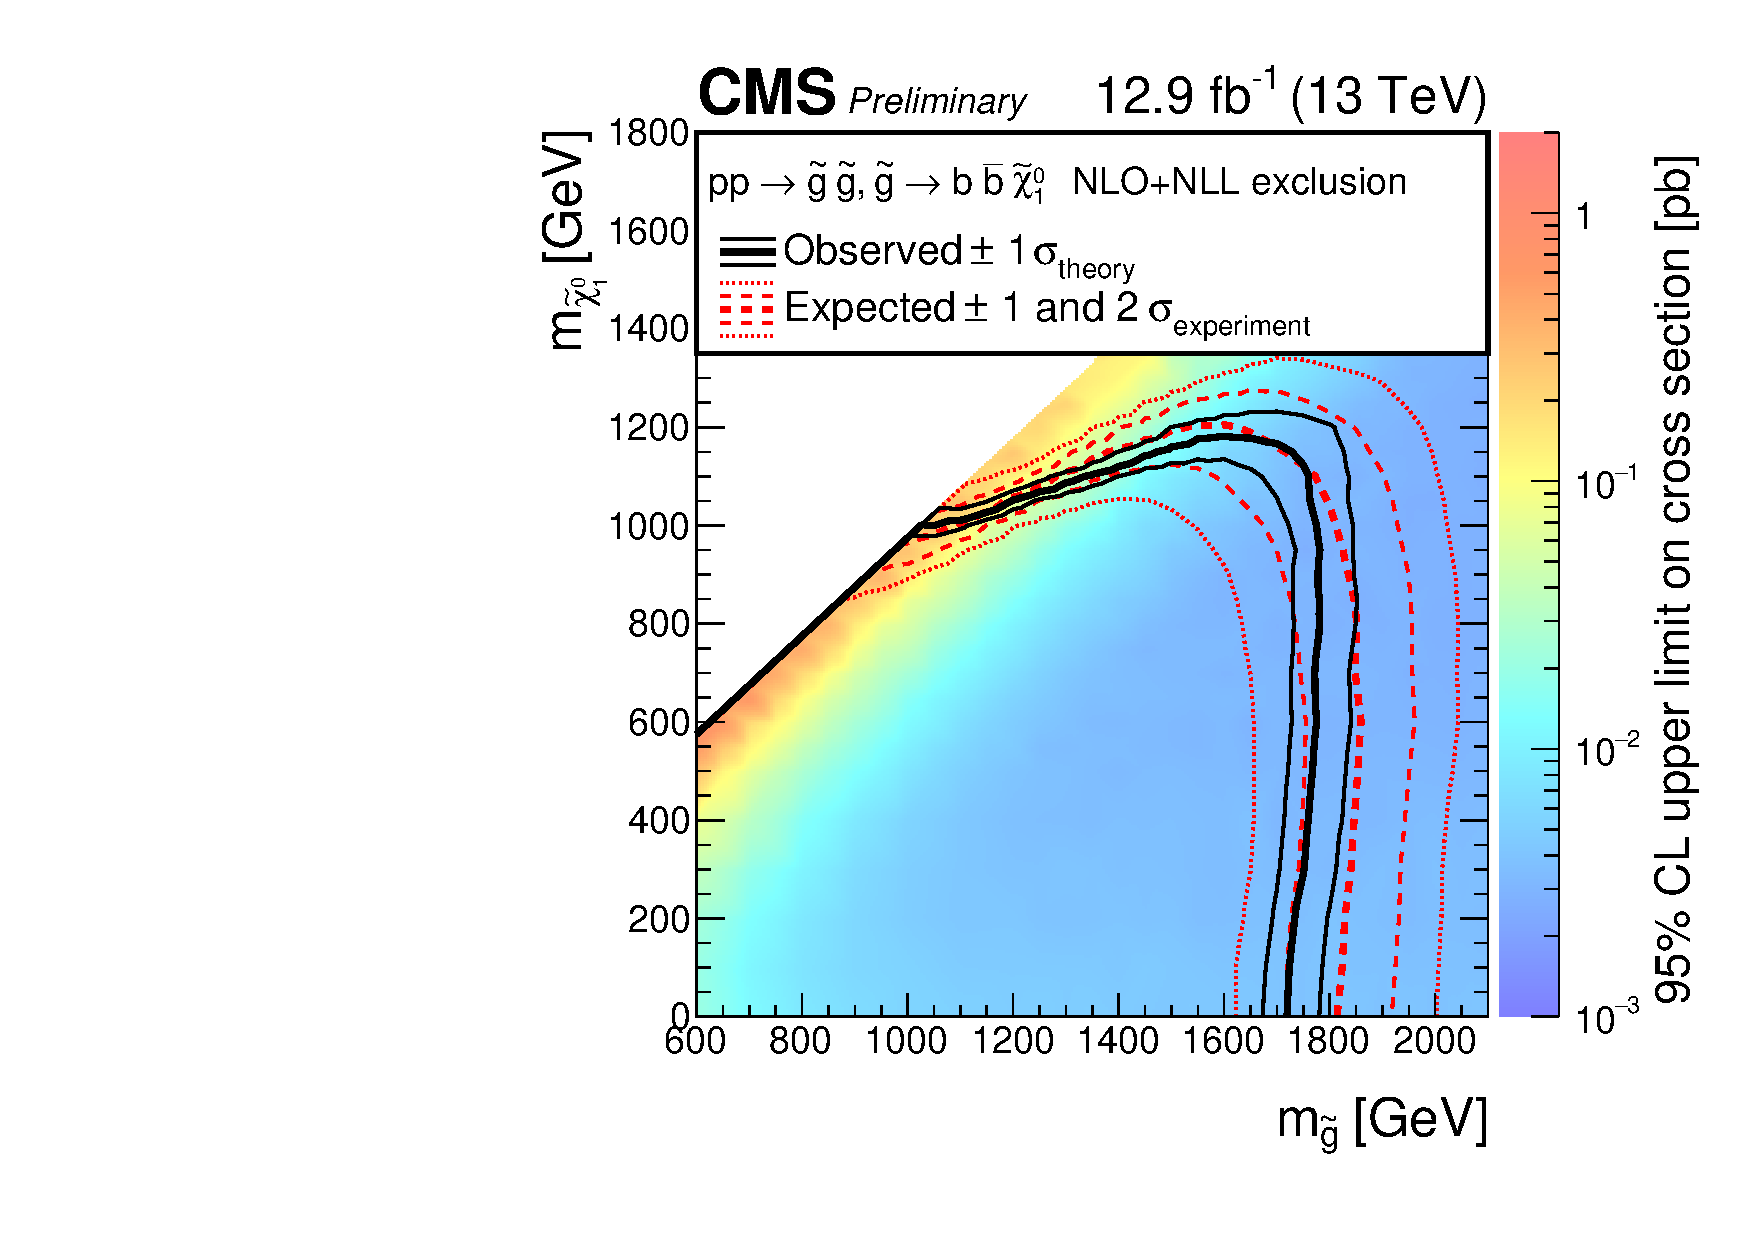
\includegraphics[width=0.6\textwidth]{figures/susyResults13/T1bbbbXSEC}
      \label{fig:T1bbbb_excl}
    } \\
    % \subfigure[T1bbbb: $\epsilon_{sig}^{\mathrm{4\,cat}}$]{
    %   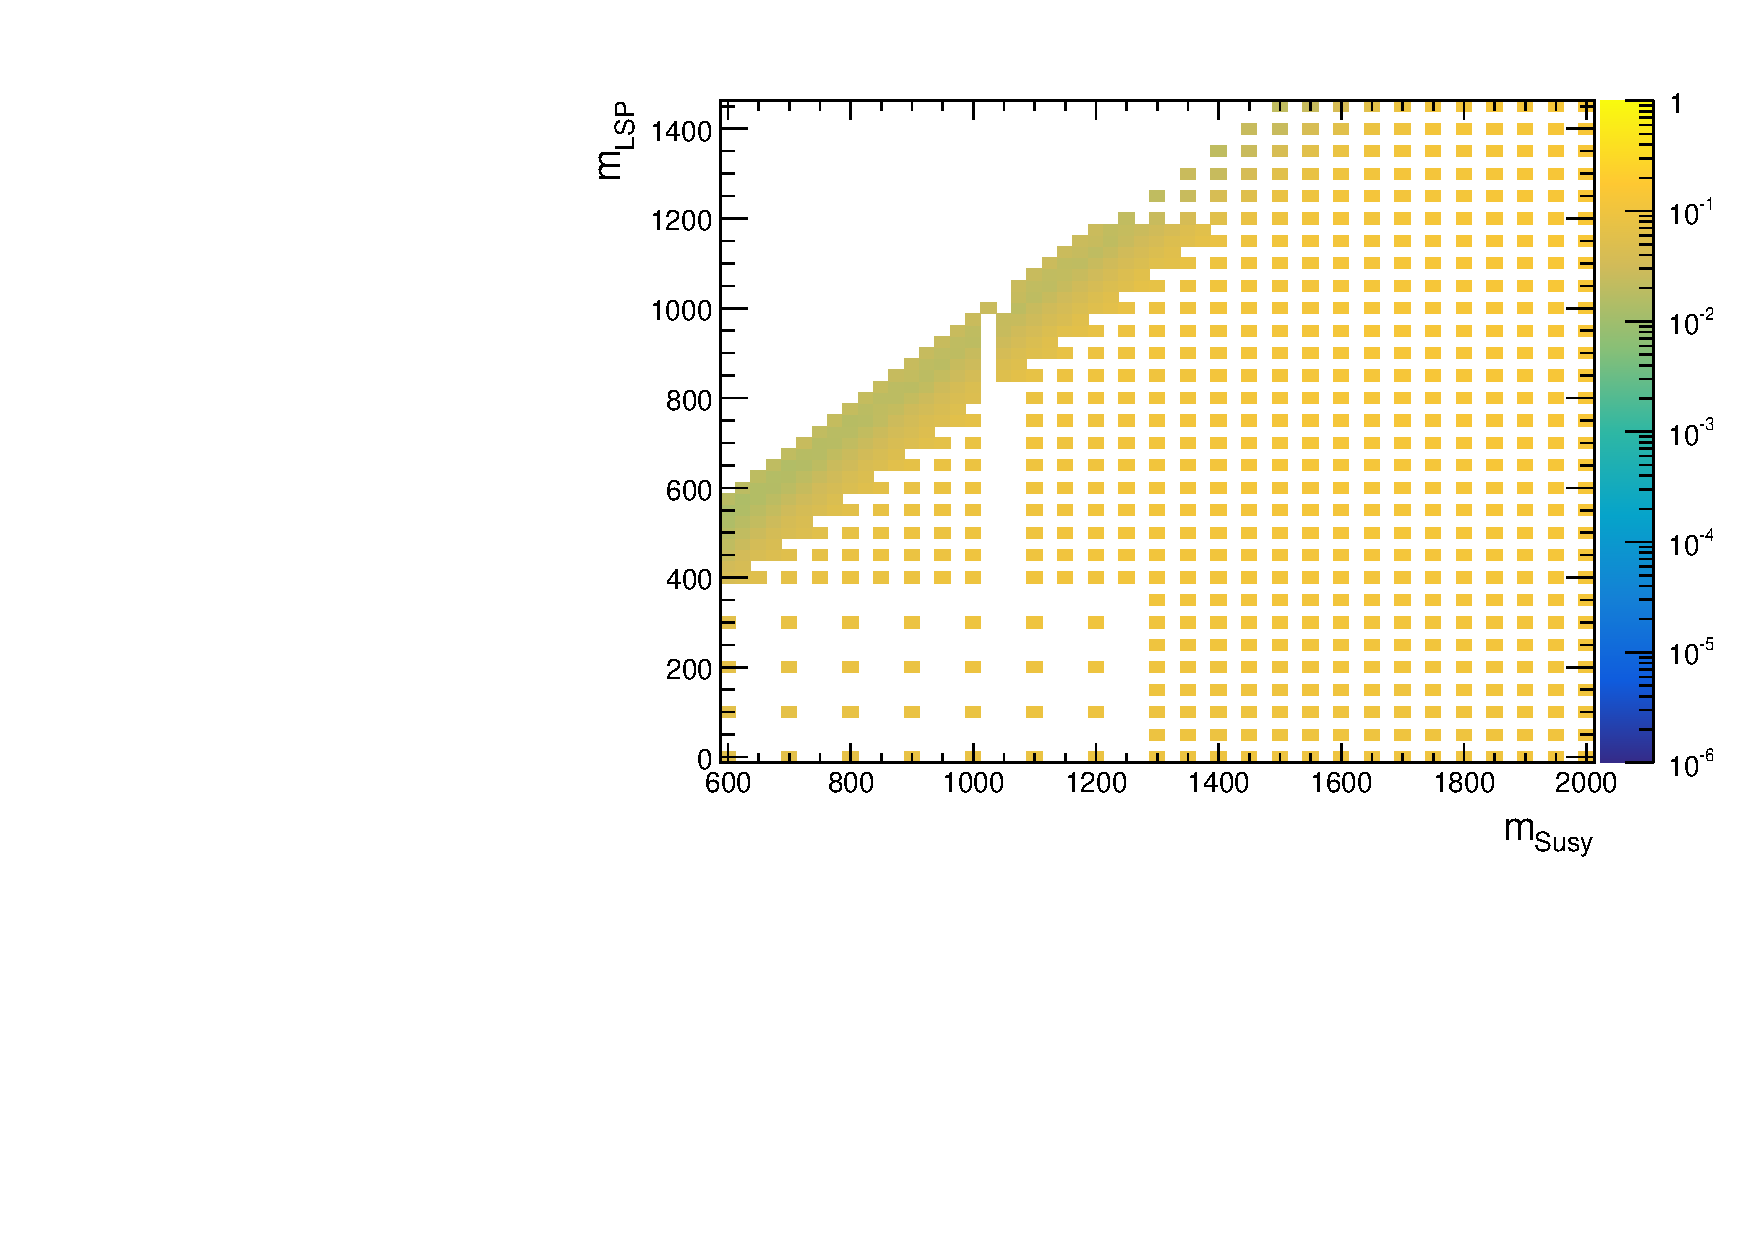
\includegraphics[width=0.45\textwidth]{figures/jetRanking/T1bbbb/eff/T1bbbb_merging_4_cats}
    %   \label{fig:T1bbbb_eff}
    % } ~~
    % \subfigure[T1bbbb: $\epsilon_{sig}^{\mathrm{4\,cat}}/\epsilon_{sig}^{\mathrm{tot}}$]{
    %   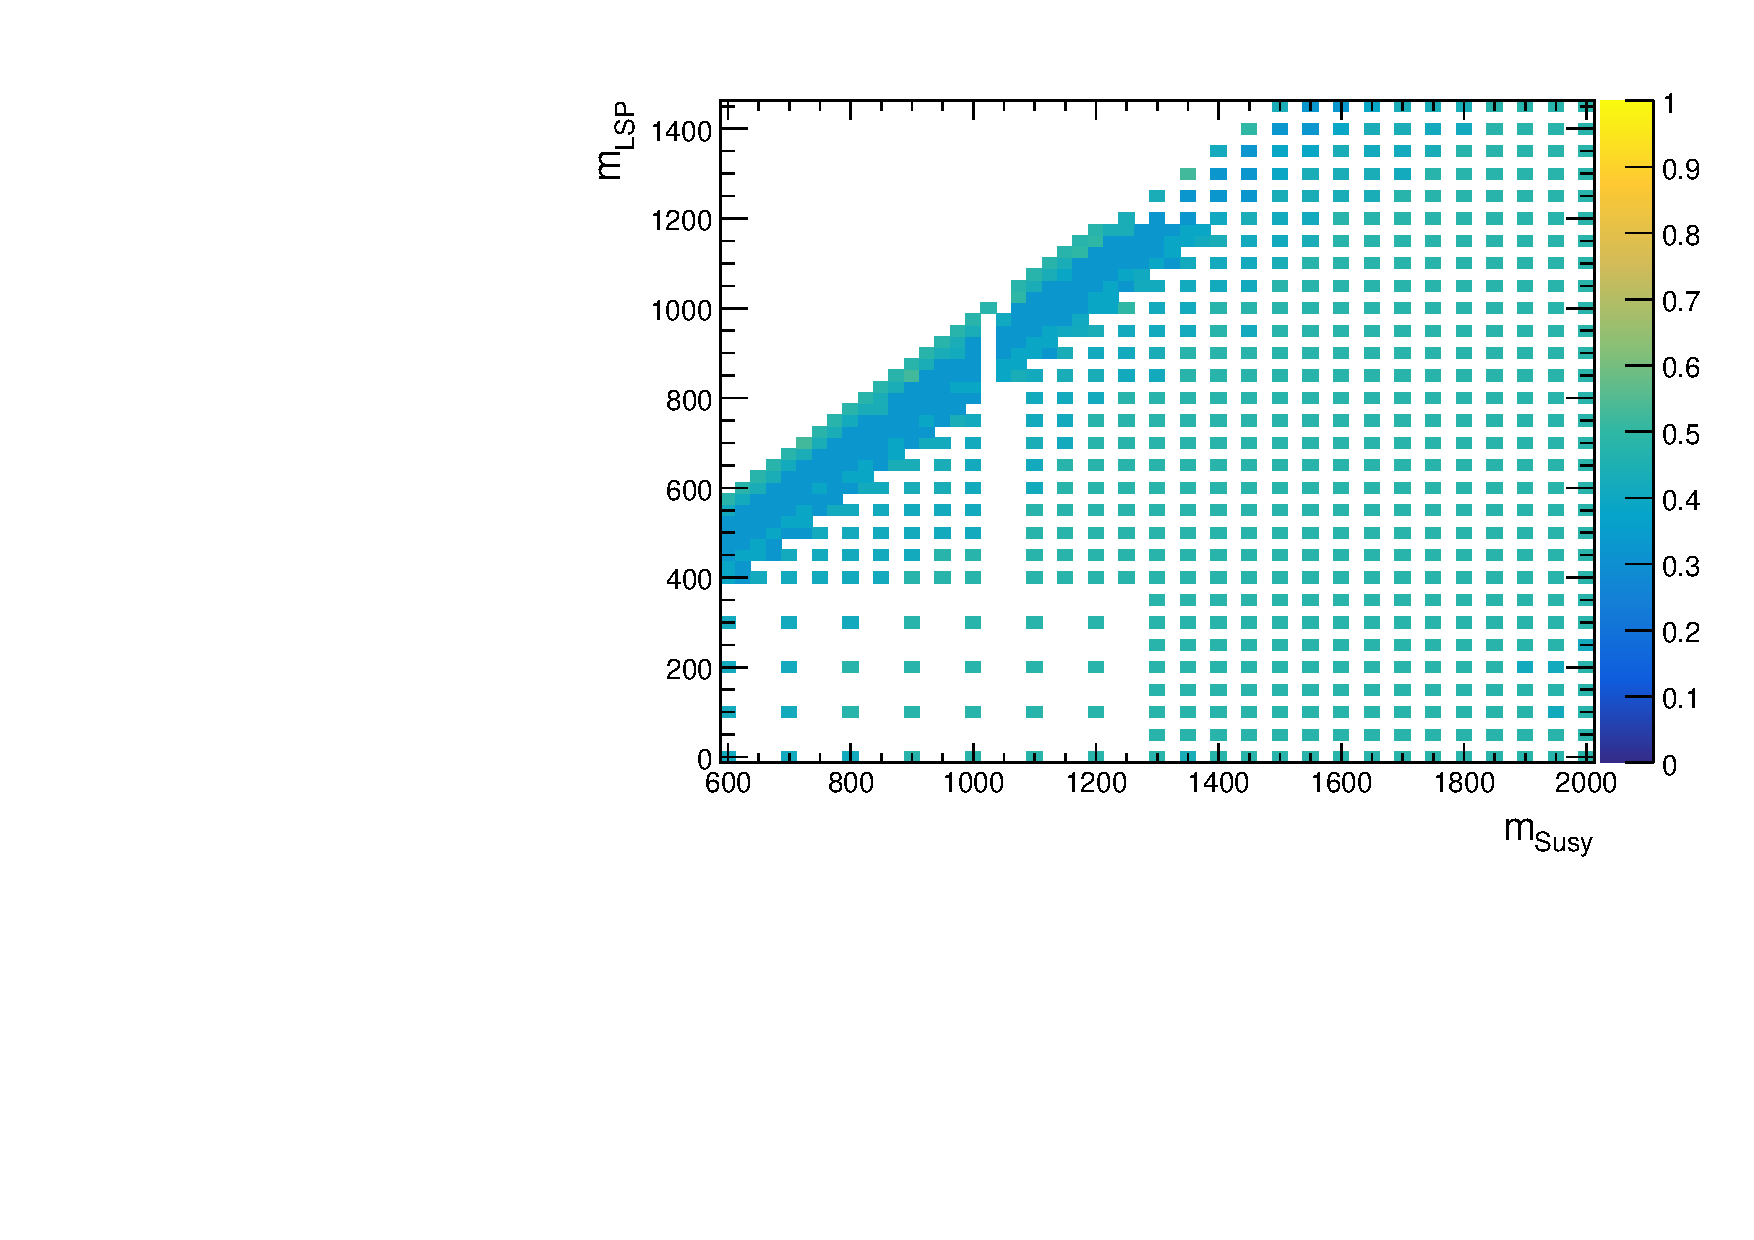
\includegraphics[width=0.45\textwidth]{figures/susyResults/T1bbbb_doubleRatioAcceptance}
    %   \label{fig:T1bbbb_eff_doubleRatio}
    % }
    \caption{
      The 95\% C.L. observed upper limit on the cross section (histogram), with the expected (solid black line) observed (solid red line) exclusion contours. 
      % Bottom left: signal acceptance including the 4 most excluding jet categories. 
      % Bottom right: ratio of the signal acceptance including 4 categories to the acceptance including the whole signal region. 
    }
    \label{fig:T1bbbb}
  \end{center}
\end{figure}

\newpage
\begin{figure}[h!]
  \begin{center}
    \subfigure[T1qqqq: Upper limit on the cross section in the $(m_{\mathrm{Gluino}},m_{\mathrm{Susy}})$ plane]{
      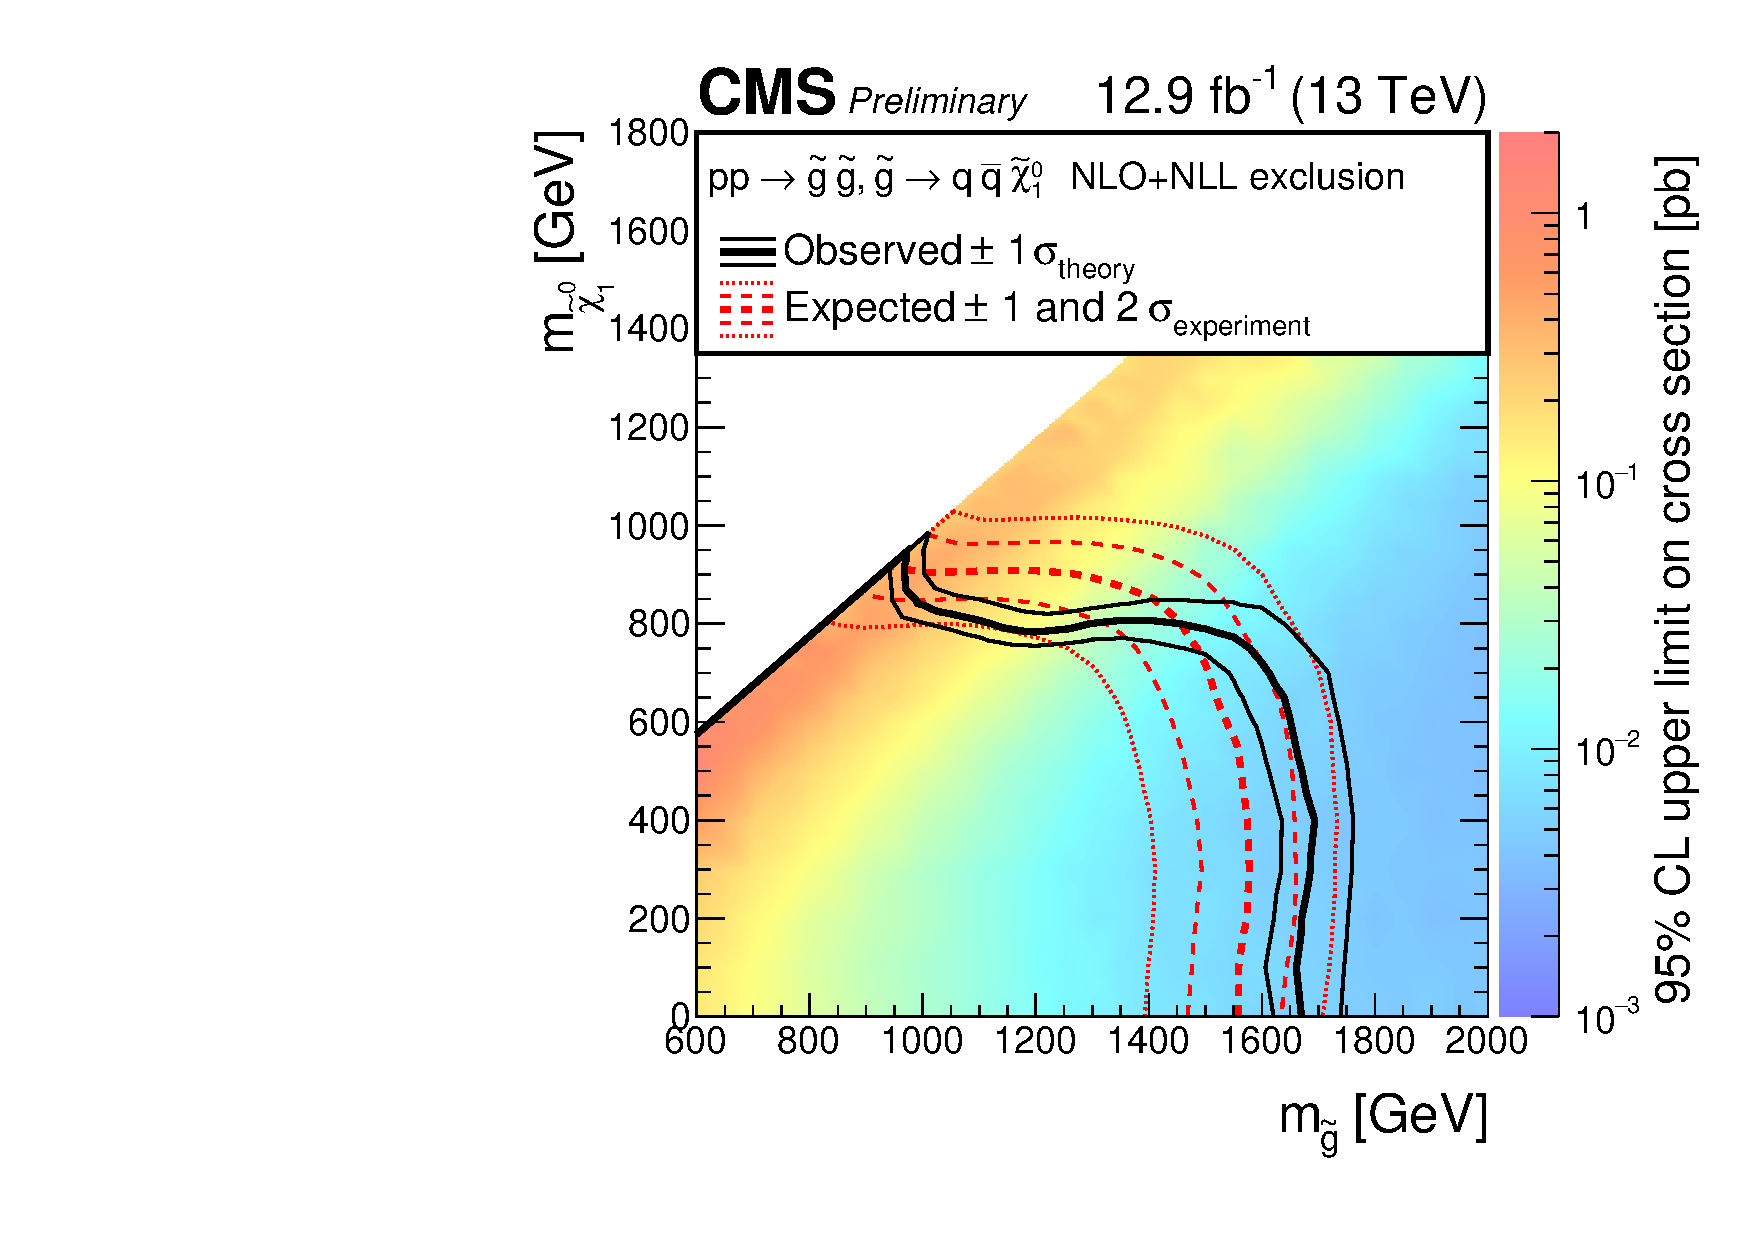
\includegraphics[width=0.6\textwidth]{figures/susyResults13/T1qqqqXSEC}
      \label{fig:T1qqqq_excl}
    } \\
    % \subfigure[T1qqqq: $\epsilon_{sig}^{\mathrm{4\,cat}}$]{
    %   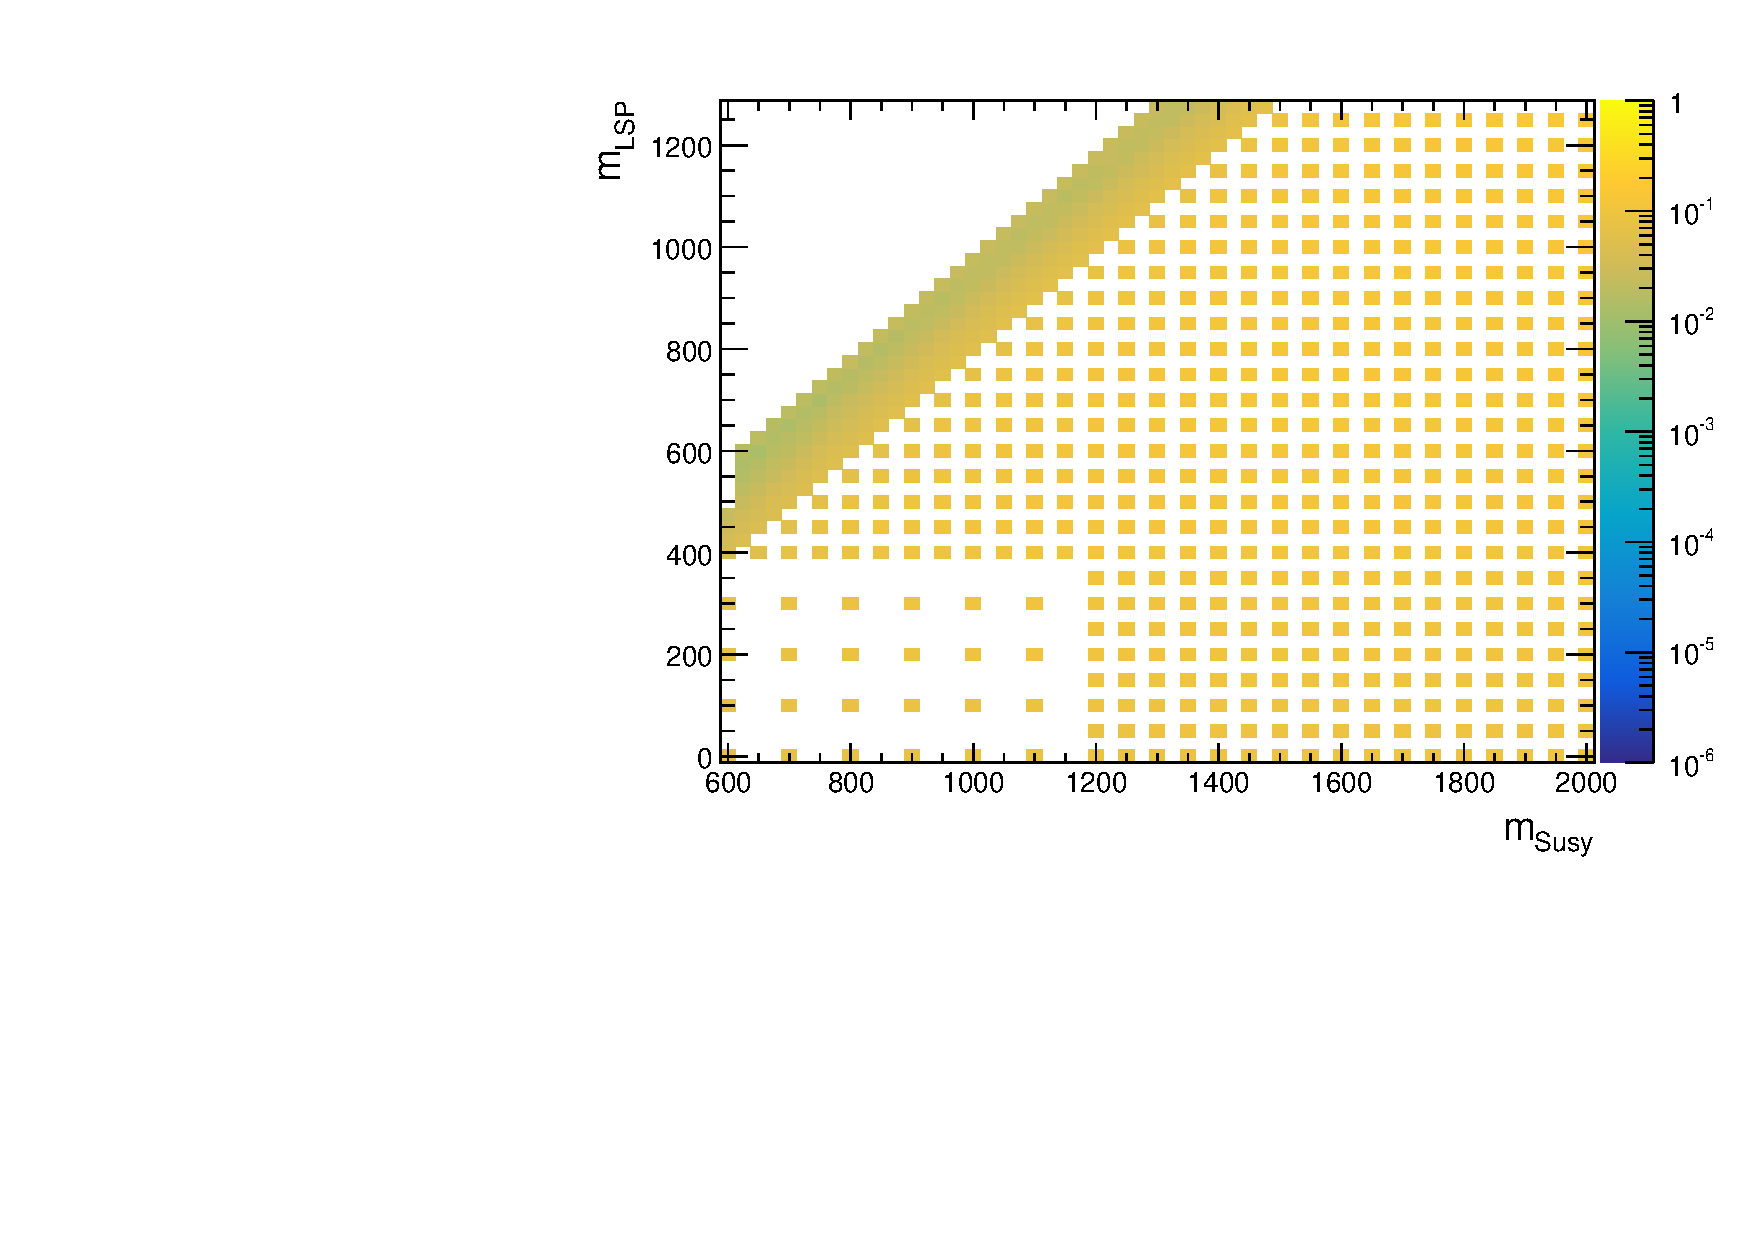
\includegraphics[width=0.45\textwidth]{figures/jetRanking/T1qqqq/eff/T1qqqq_merging_4_cats}
    %   \label{fig:T1qqqq_eff}
    % } ~~
    % \subfigure[T1qqqq: $\epsilon_{sig}^{\mathrm{4\,cat}}/\epsilon_{sig}^{\mathrm{tot}}$]{
    %   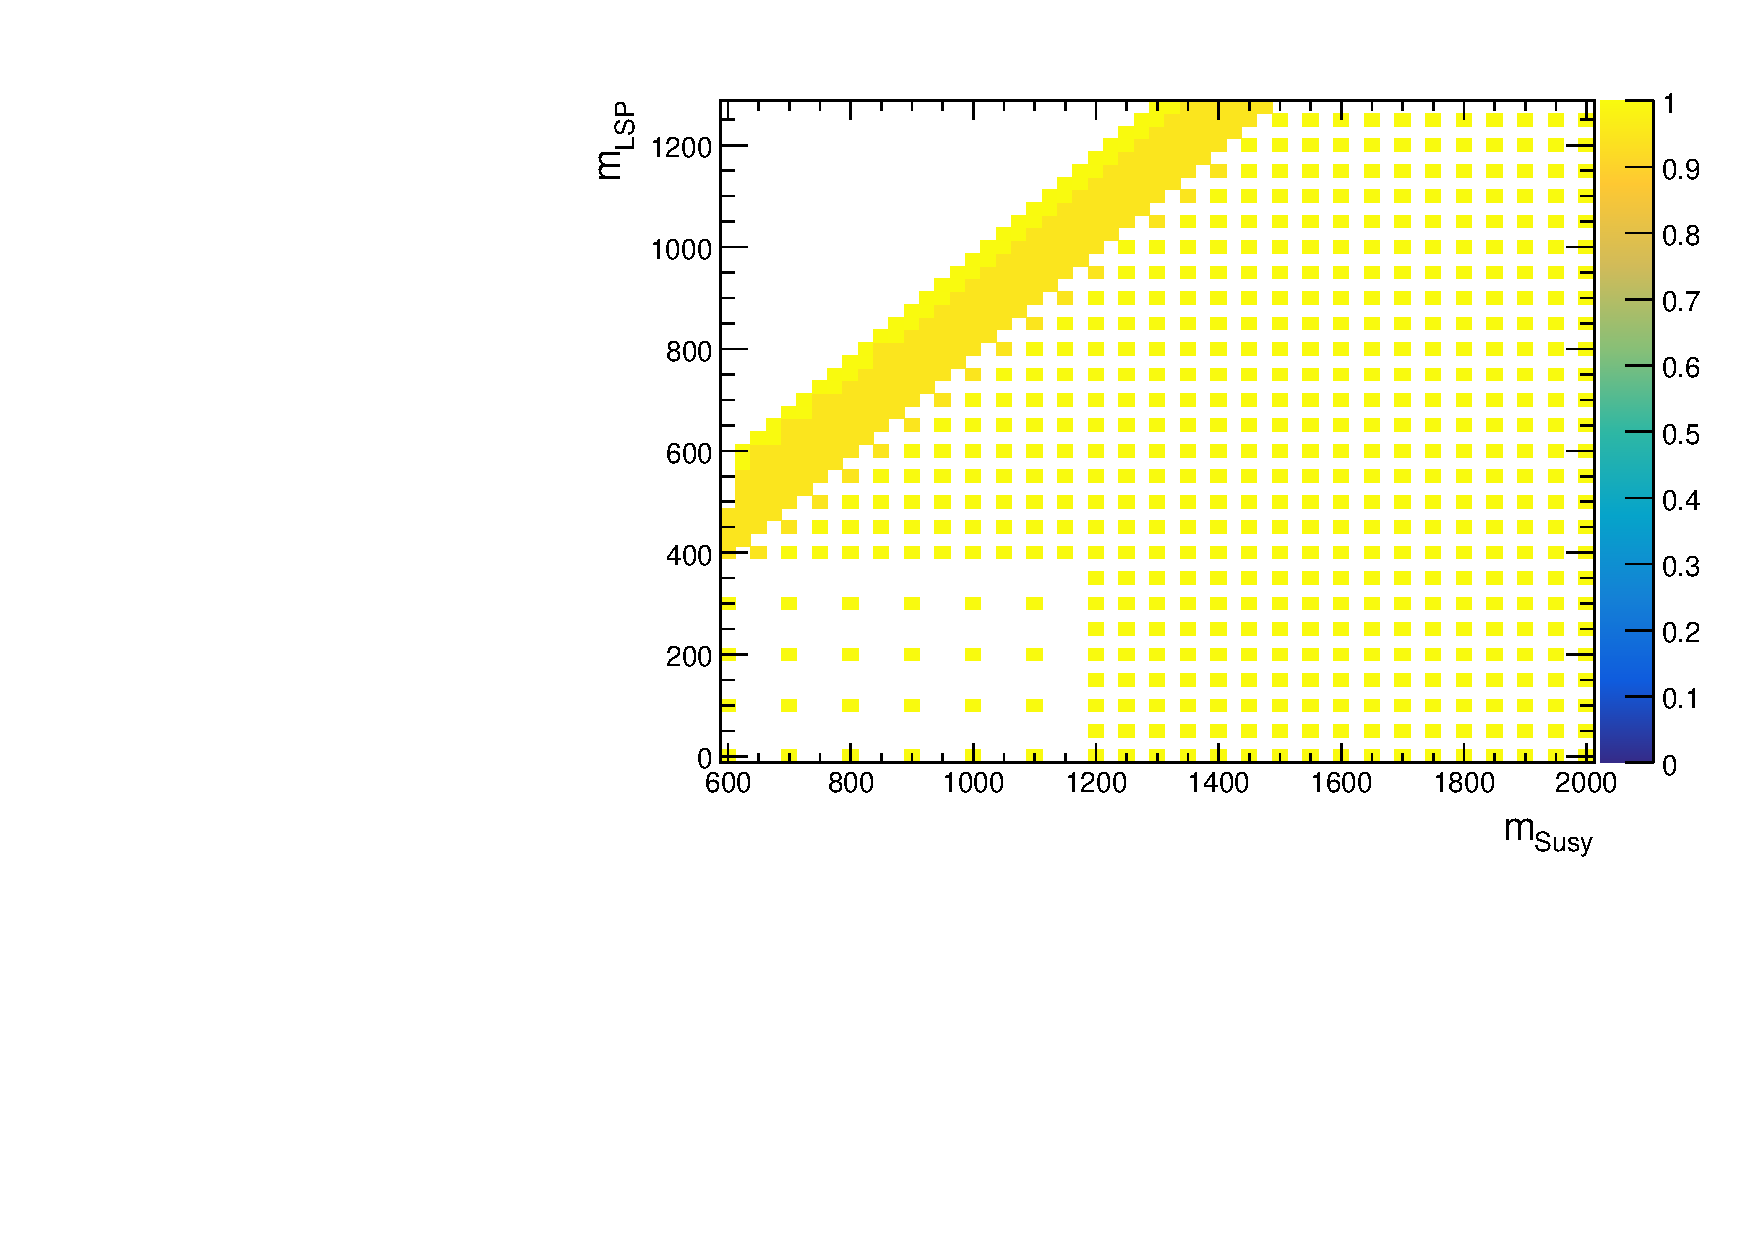
\includegraphics[width=0.45\textwidth]{figures/susyResults/T1qqqq_doubleRatioAcceptance}
    %   \label{fig:T1qqqq_eff_doubleRatio}
    % }
    \caption{
      The 95\% C.L. observed upper limit on the cross section (histogram), with the expected (solid black line) observed (solid red line) exclusion contours. 
      % Bottom left: signal acceptance including the 4 most excluding jet categories. 
      % Bottom right: ratio of the signal acceptance including 4 categories to the acceptance including the whole signal region. 
    }
    \label{fig:T1qqqq}
  \end{center}
\end{figure}

%% \newpage
%% \begin{figure}[h!]
%%   \begin{center}
%%     \subfigure[T1ttbb: Upper limit on the cross section in the $(m_{\mathrm{Gluino}},m_{\mathrm{Susy}})$ plane]{
%%       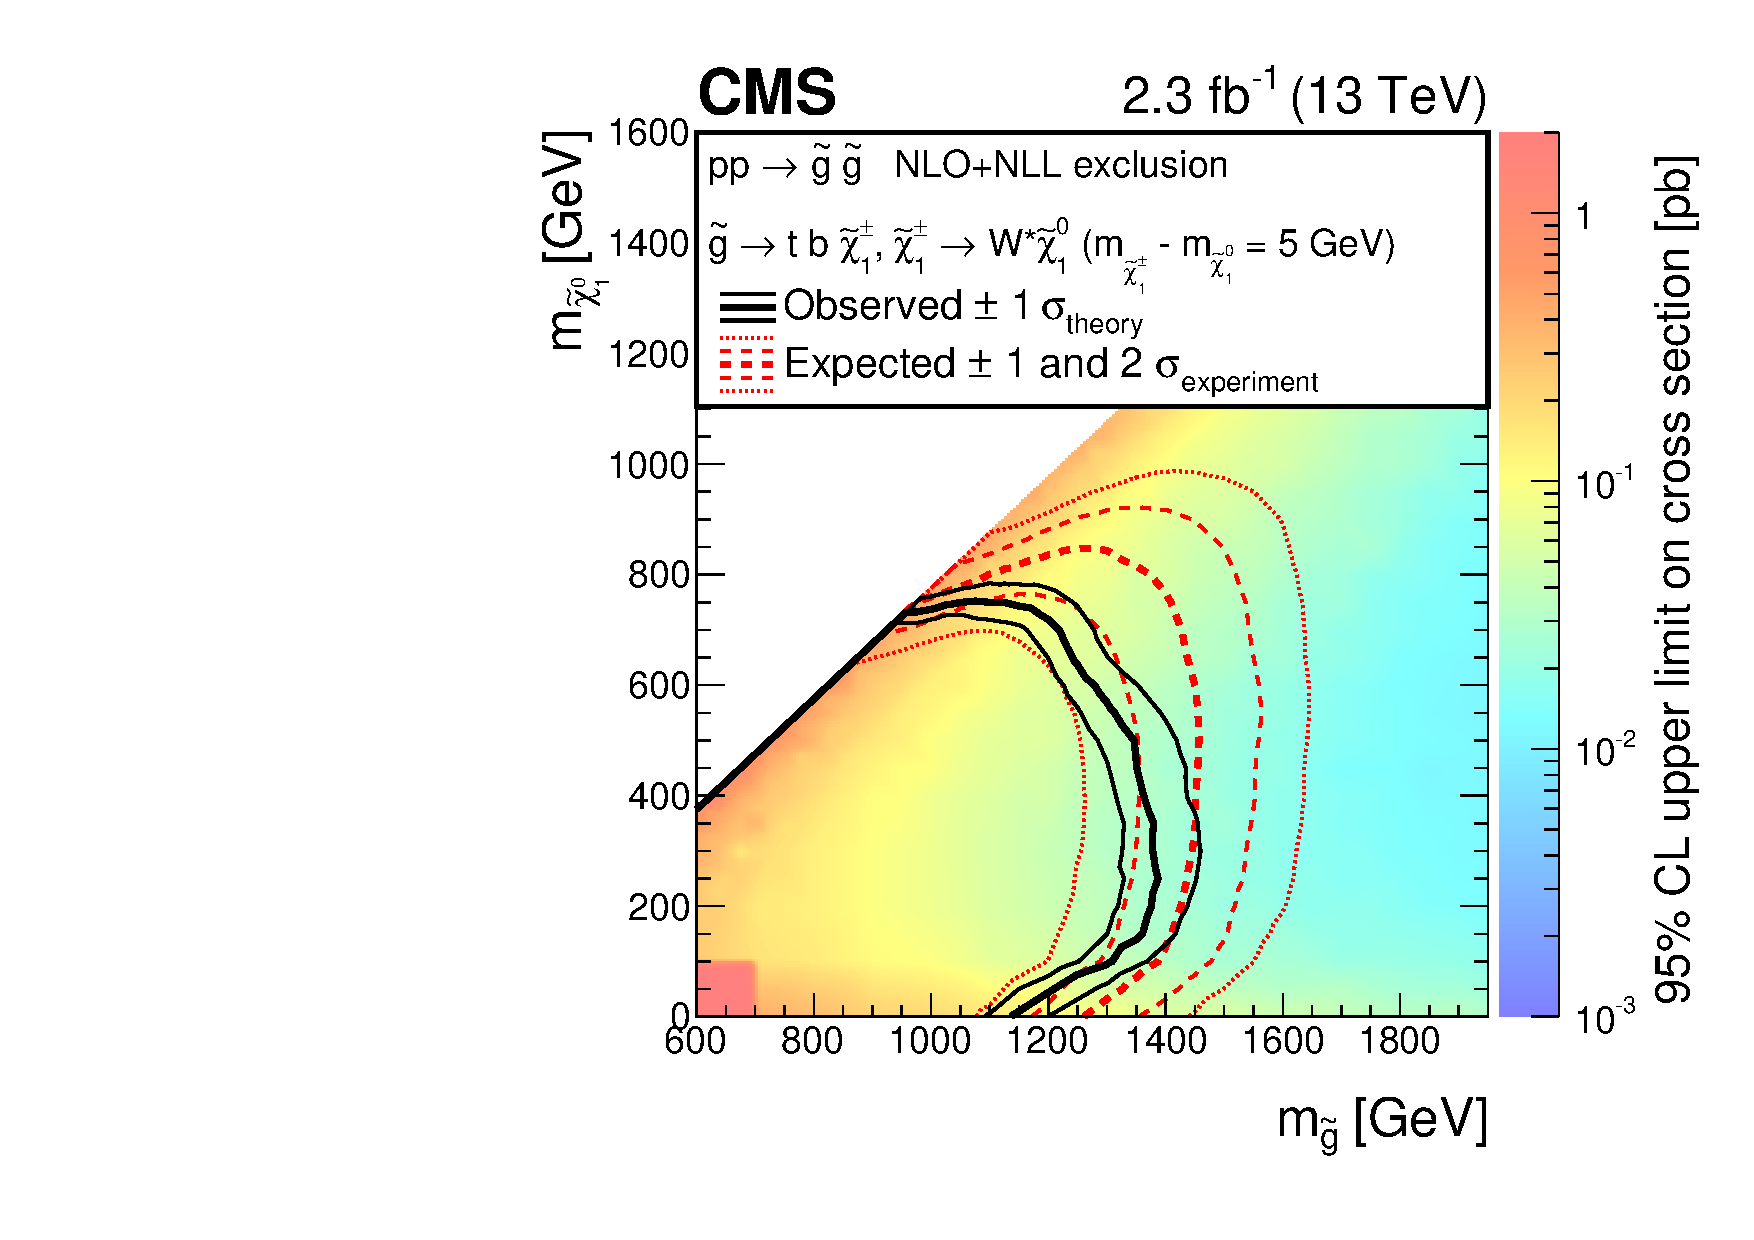
\includegraphics[width=0.6\textwidth]{figures/susyResults/T1ttbbXSEC}
%%       \label{fig:T1ttbb_excl}
%%     } \\
%%     \subfigure[T1ttbb: $\epsilon_{sig}^{\mathrm{4\,cat}}$]{
%%       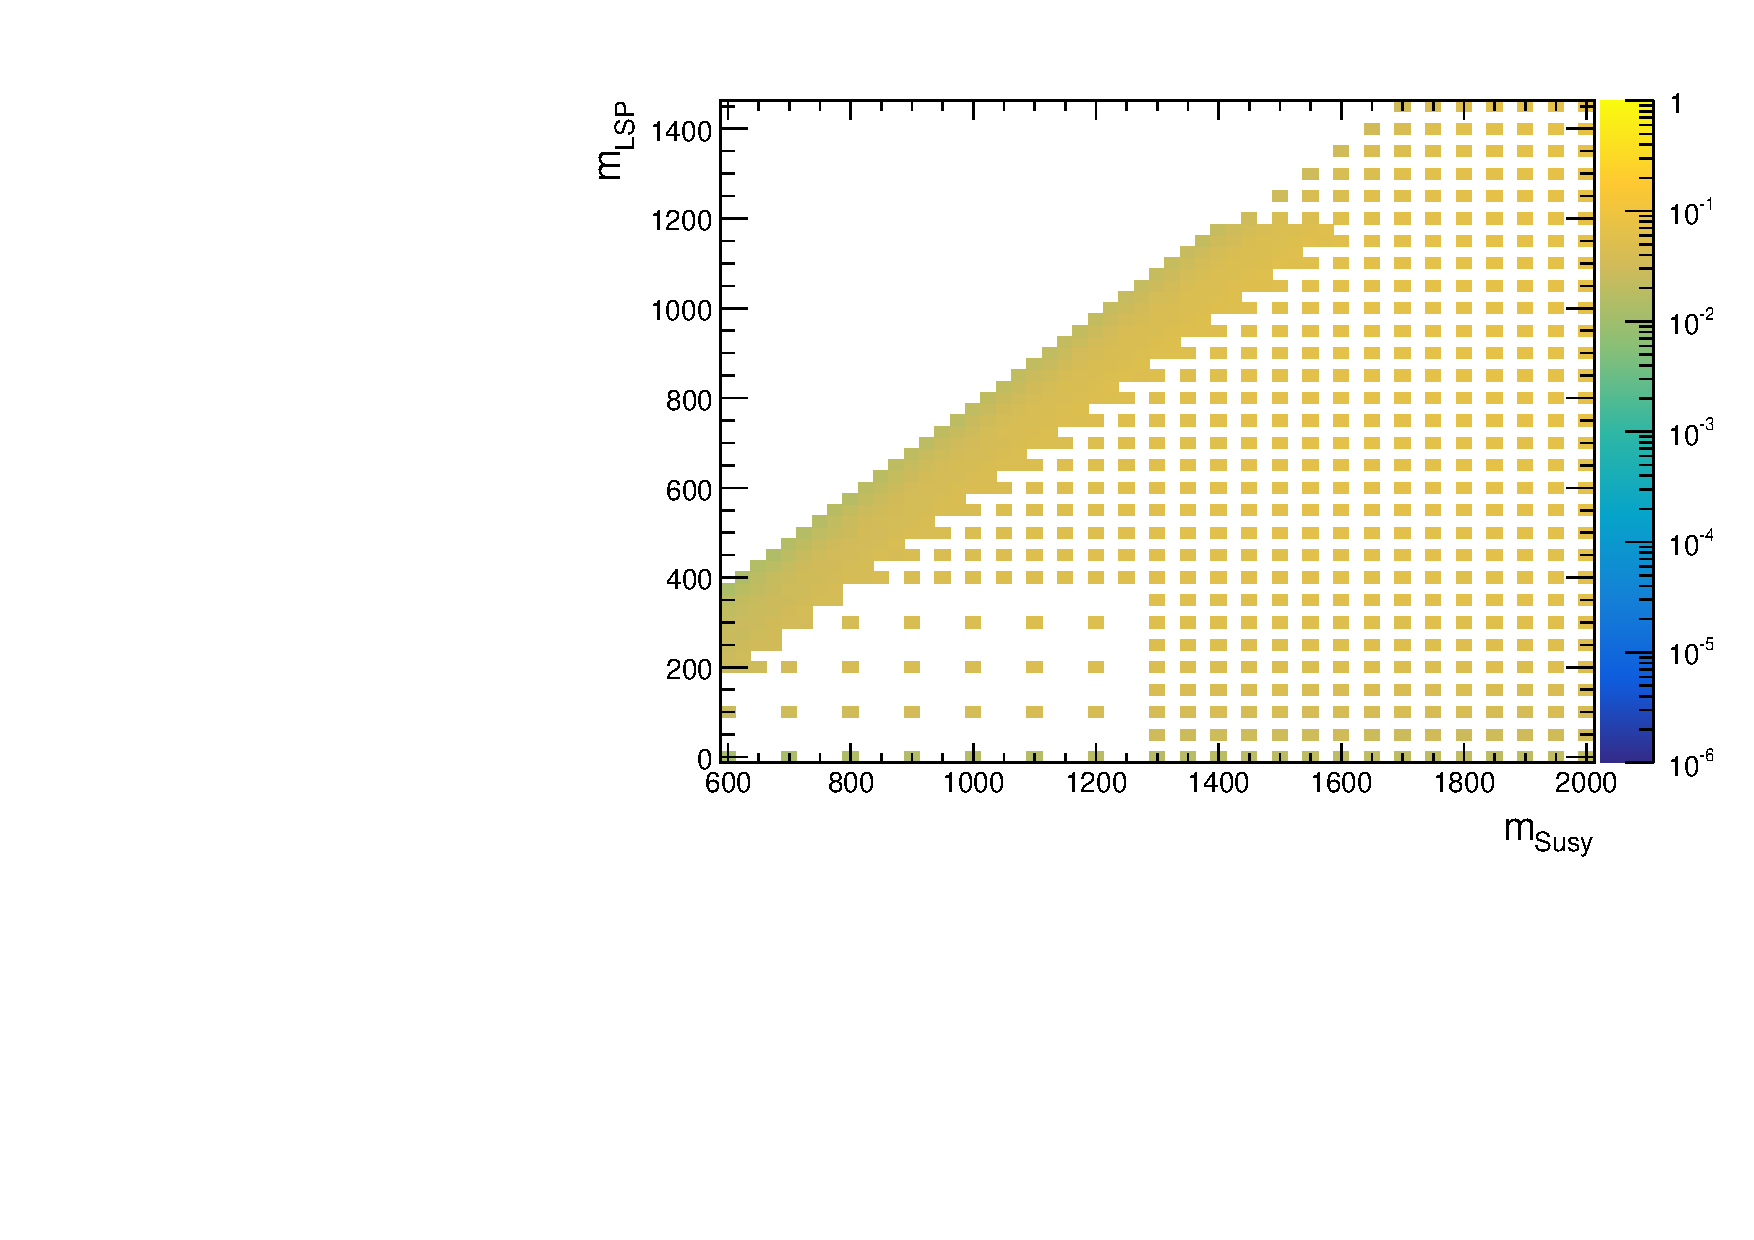
\includegraphics[width=0.45\textwidth]{figures/jetRanking/T1ttbb/eff/T1ttbb_merging_4_cats}
%%       \label{fig:T1ttbb_eff}
%%     } ~~
%%     \subfigure[T1ttbb: $\epsilon_{sig}^{\mathrm{4\,cat}}/\epsilon_{sig}^{\mathrm{tot}}$]{
%%       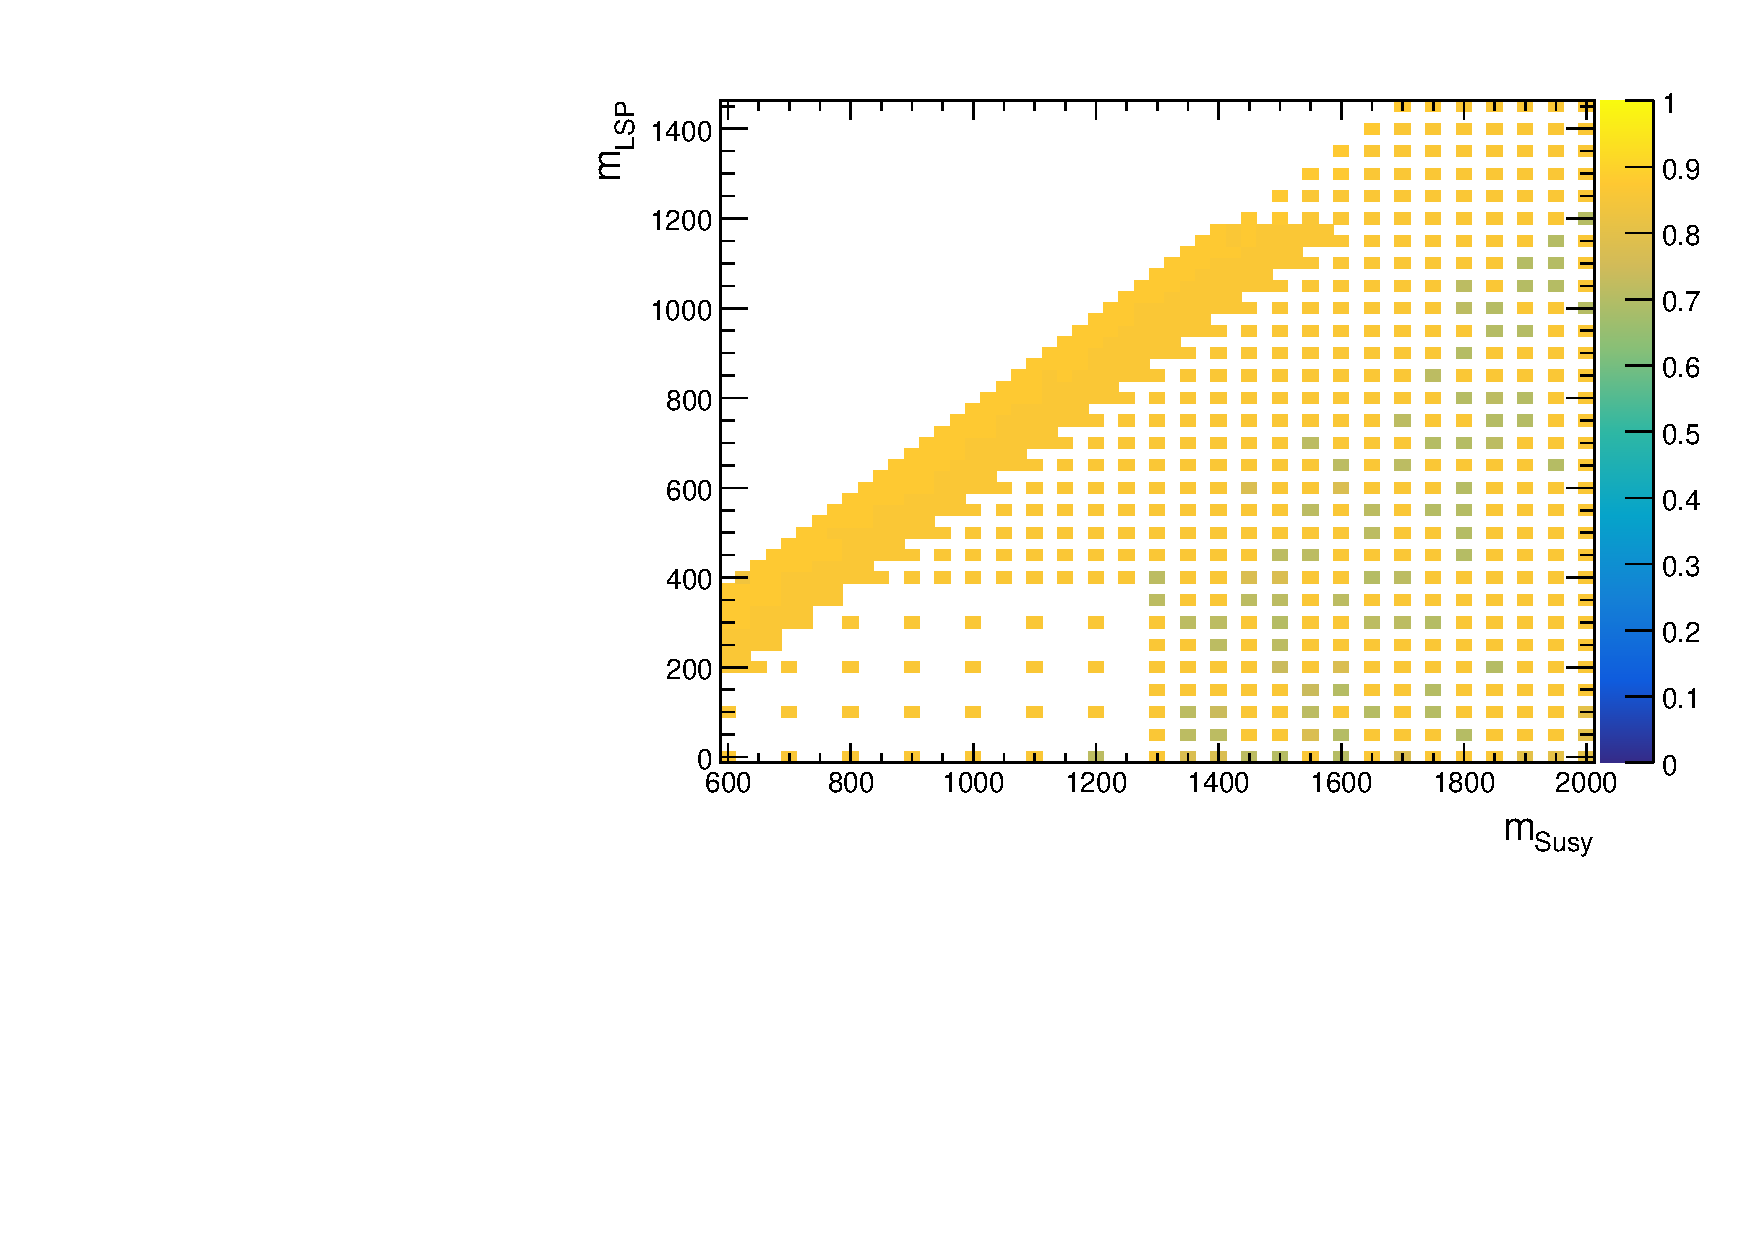
\includegraphics[width=0.45\textwidth]{figures/susyResults/T1ttbb_doubleRatioAcceptance}
%%       \label{fig:T1ttbb_eff_doubleRatio}
%%     }
%%     \caption{
%%       Top: the 95\% C.L. observed upper limit on the cross section (histogram), with the expected (solid black line) observed (solid red line) exclusion contours. 
%%       Bottom left: signal acceptance including the 4 most excluding jet categories. 
%%       Bottom right: ratio of the signal acceptance including 4 categories to the acceptance including the whole signal region. 
%%     }
%%     \label{fig:T1ttbb}
%%   \end{center}
%% \end{figure}


%% \newpage
%% \begin{figure}[h!]
%%   \begin{center}
%%     \subfigure[T5ttcc: Upper limit on the cross section in the $(m_{\mathrm{Gluino}},m_{\mathrm{Susy}})$ plane]{
%%       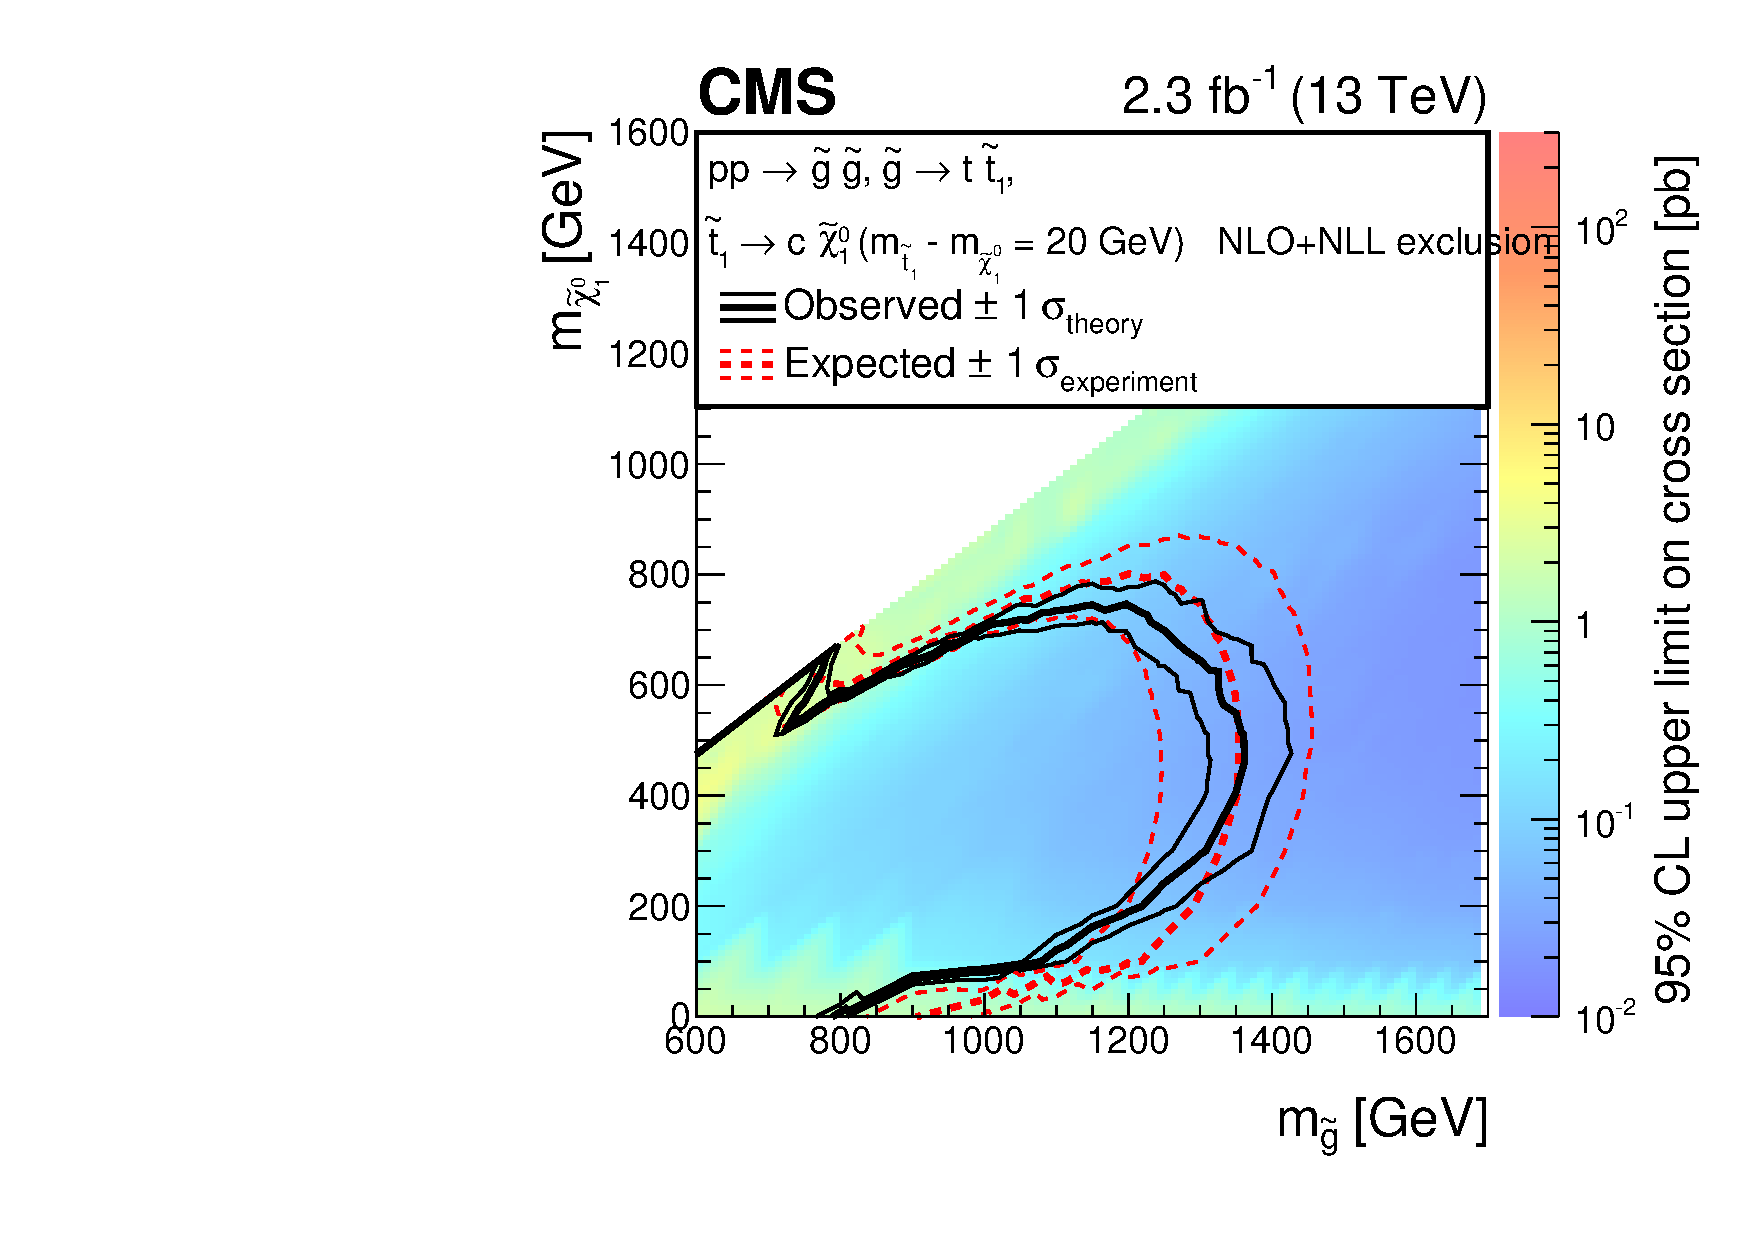
\includegraphics[width=0.6\textwidth]{figures/susyResults/T5ttccXSEC}
%%       \label{fig:T5ttcc_excl}
%%     } \\
%%     \subfigure[T5ttcc: $\epsilon_{sig}^{\mathrm{4\,cat}}$]{
%%       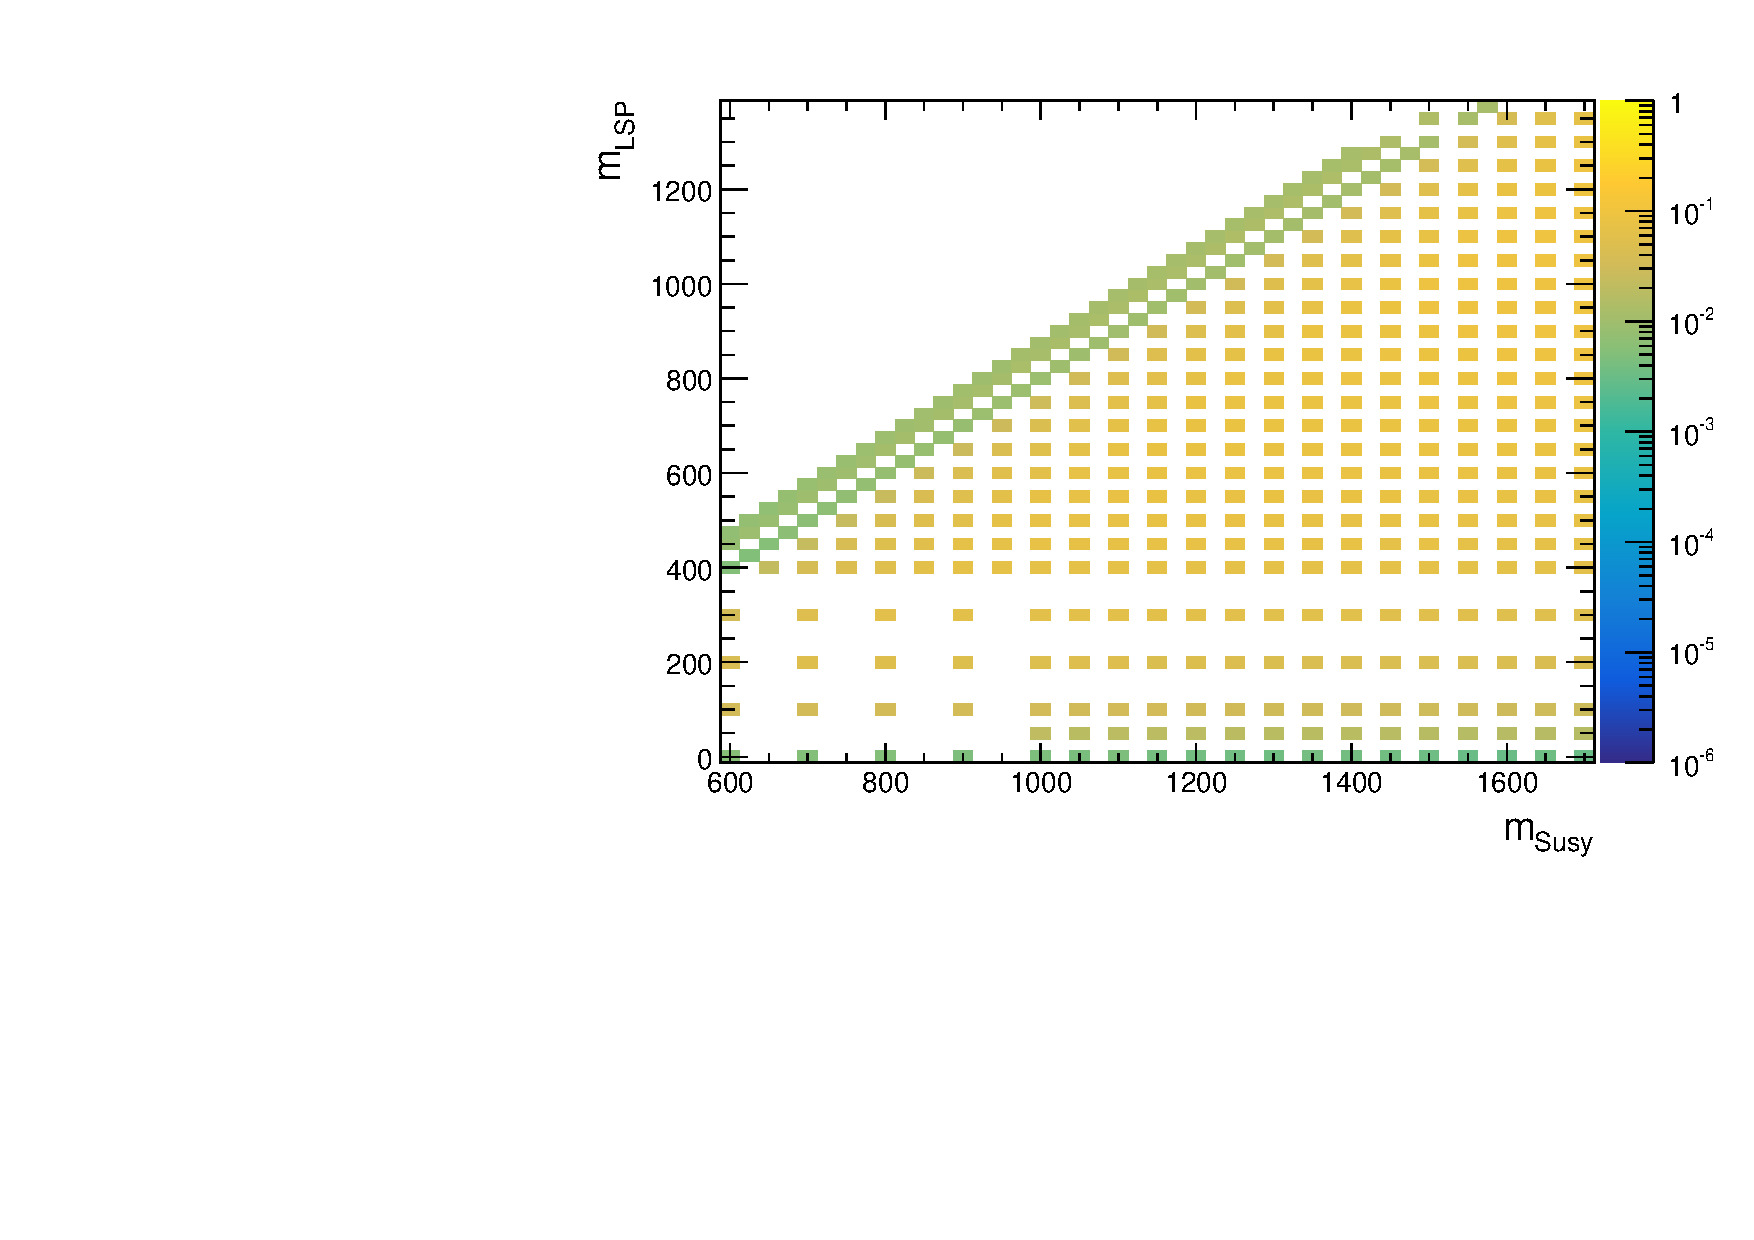
\includegraphics[width=0.45\textwidth]{figures/jetRanking/T5ttcc/eff/T5ttcc_merging_4_cats}
%%       \label{fig:T5ttcc_eff}
%%     } ~~
%%     \subfigure[T5ttcc: $\epsilon_{sig}^{\mathrm{4\,cat}}/\epsilon_{sig}^{\mathrm{tot}}$]{
%%       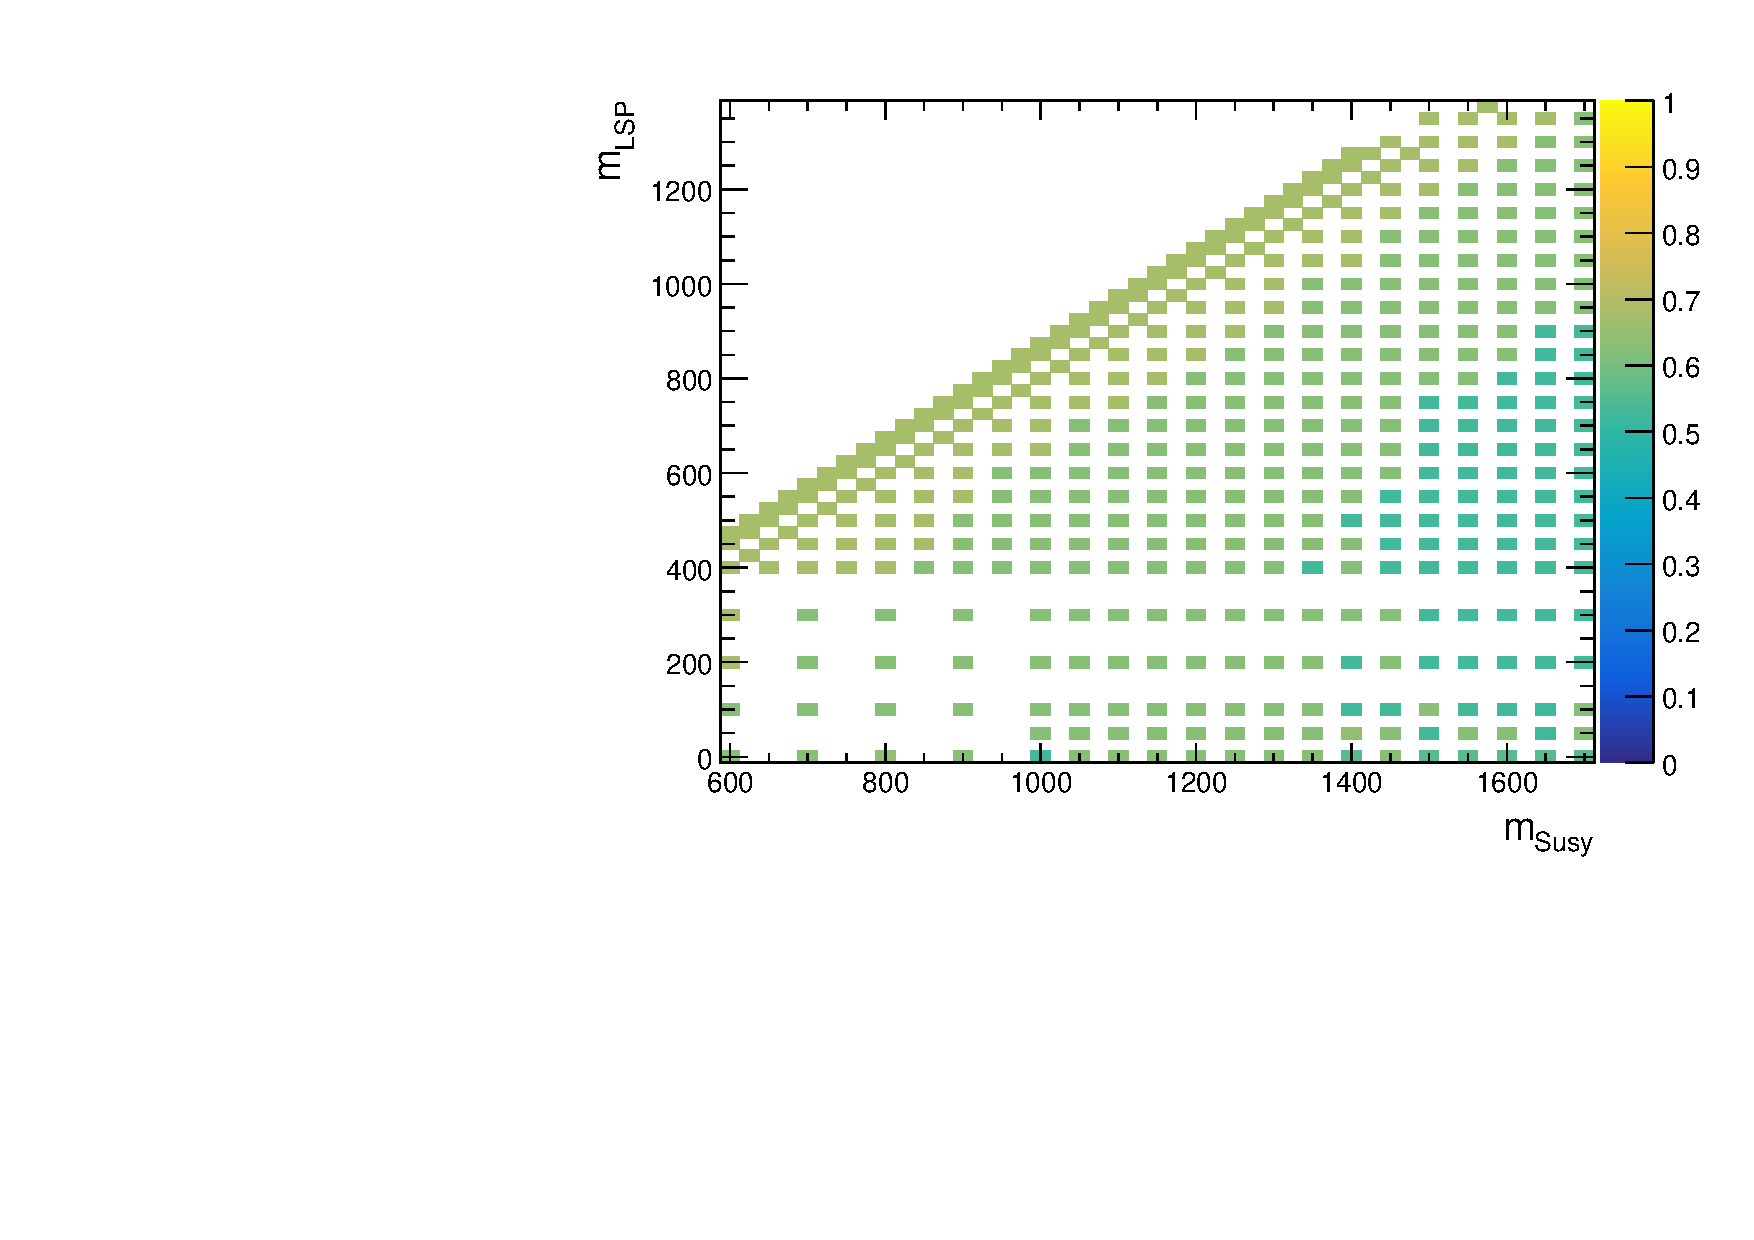
\includegraphics[width=0.45\textwidth]{figures/susyResults/T5ttcc_doubleRatioAcceptance}
%%       \label{fig:T5ttcc_eff_doubleRatio}
%%     }
%%     \caption{
%%       Top: the 95\% C.L. observed upper limit on the cross section (histogram), with the expected (solid black line) observed (solid red line) exclusion contours. 
%%       Bottom left: signal acceptance including the 4 most excluding jet categories. 
%%       Bottom right: ratio of the signal acceptance including 4 categories to the acceptance including the whole signal region. 
%%     }
%%     \label{fig:T5ttcc}
%%   \end{center}
%% \end{figure}


%% \newpage
%% \begin{figure}[h!]
%%   \begin{center}
%%     \subfigure[T5ttttDM175: Upper limit on the cross section in the $(m_{\mathrm{Gluino}},m_{\mathrm{Susy}})$ plane]{
%%       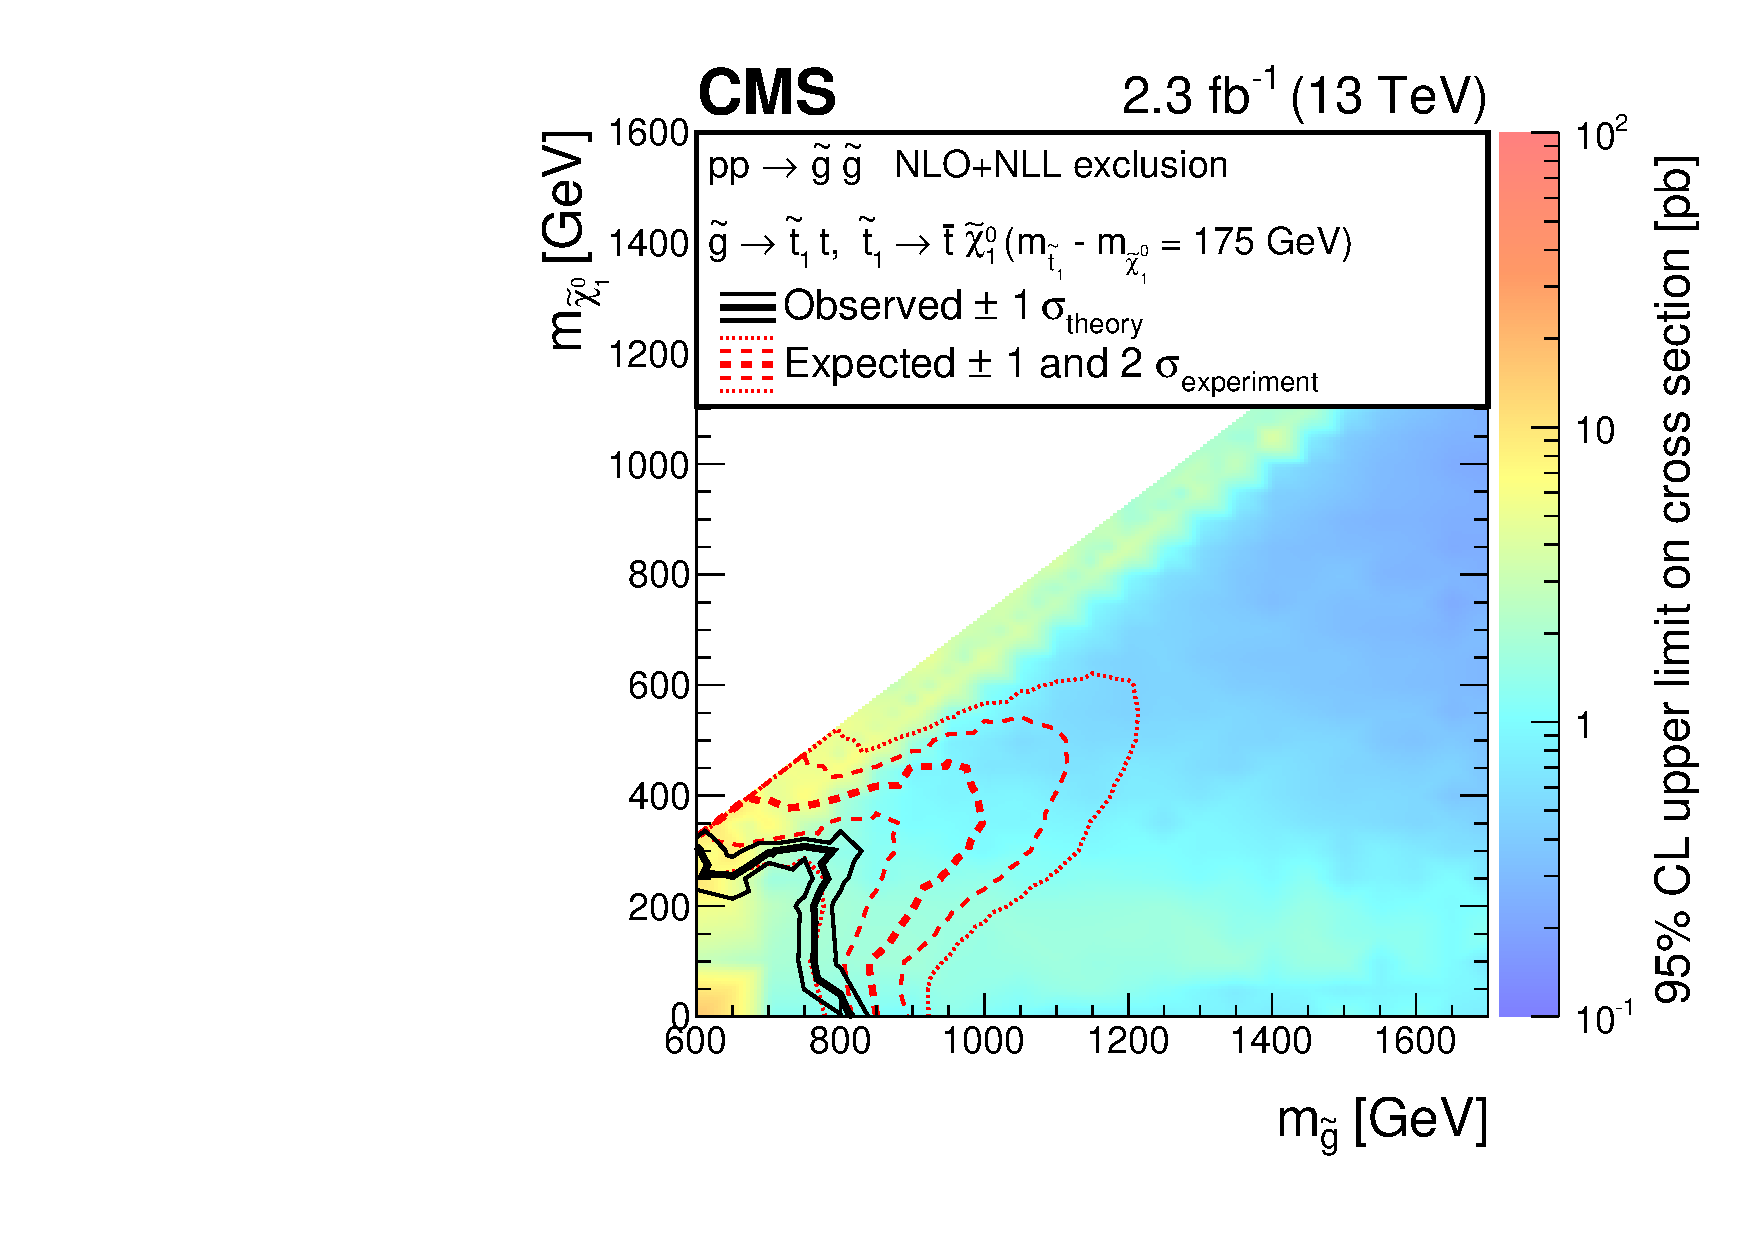
\includegraphics[width=0.6\textwidth]{figures/susyResults/T5ttttDM175XSEC}
%%       \label{fig:T5ttttDM175_excl}
%%     } \\
%%     \subfigure[T5ttttDM175: $\epsilon_{sig}^{\mathrm{4\,cat}}$]{
%%       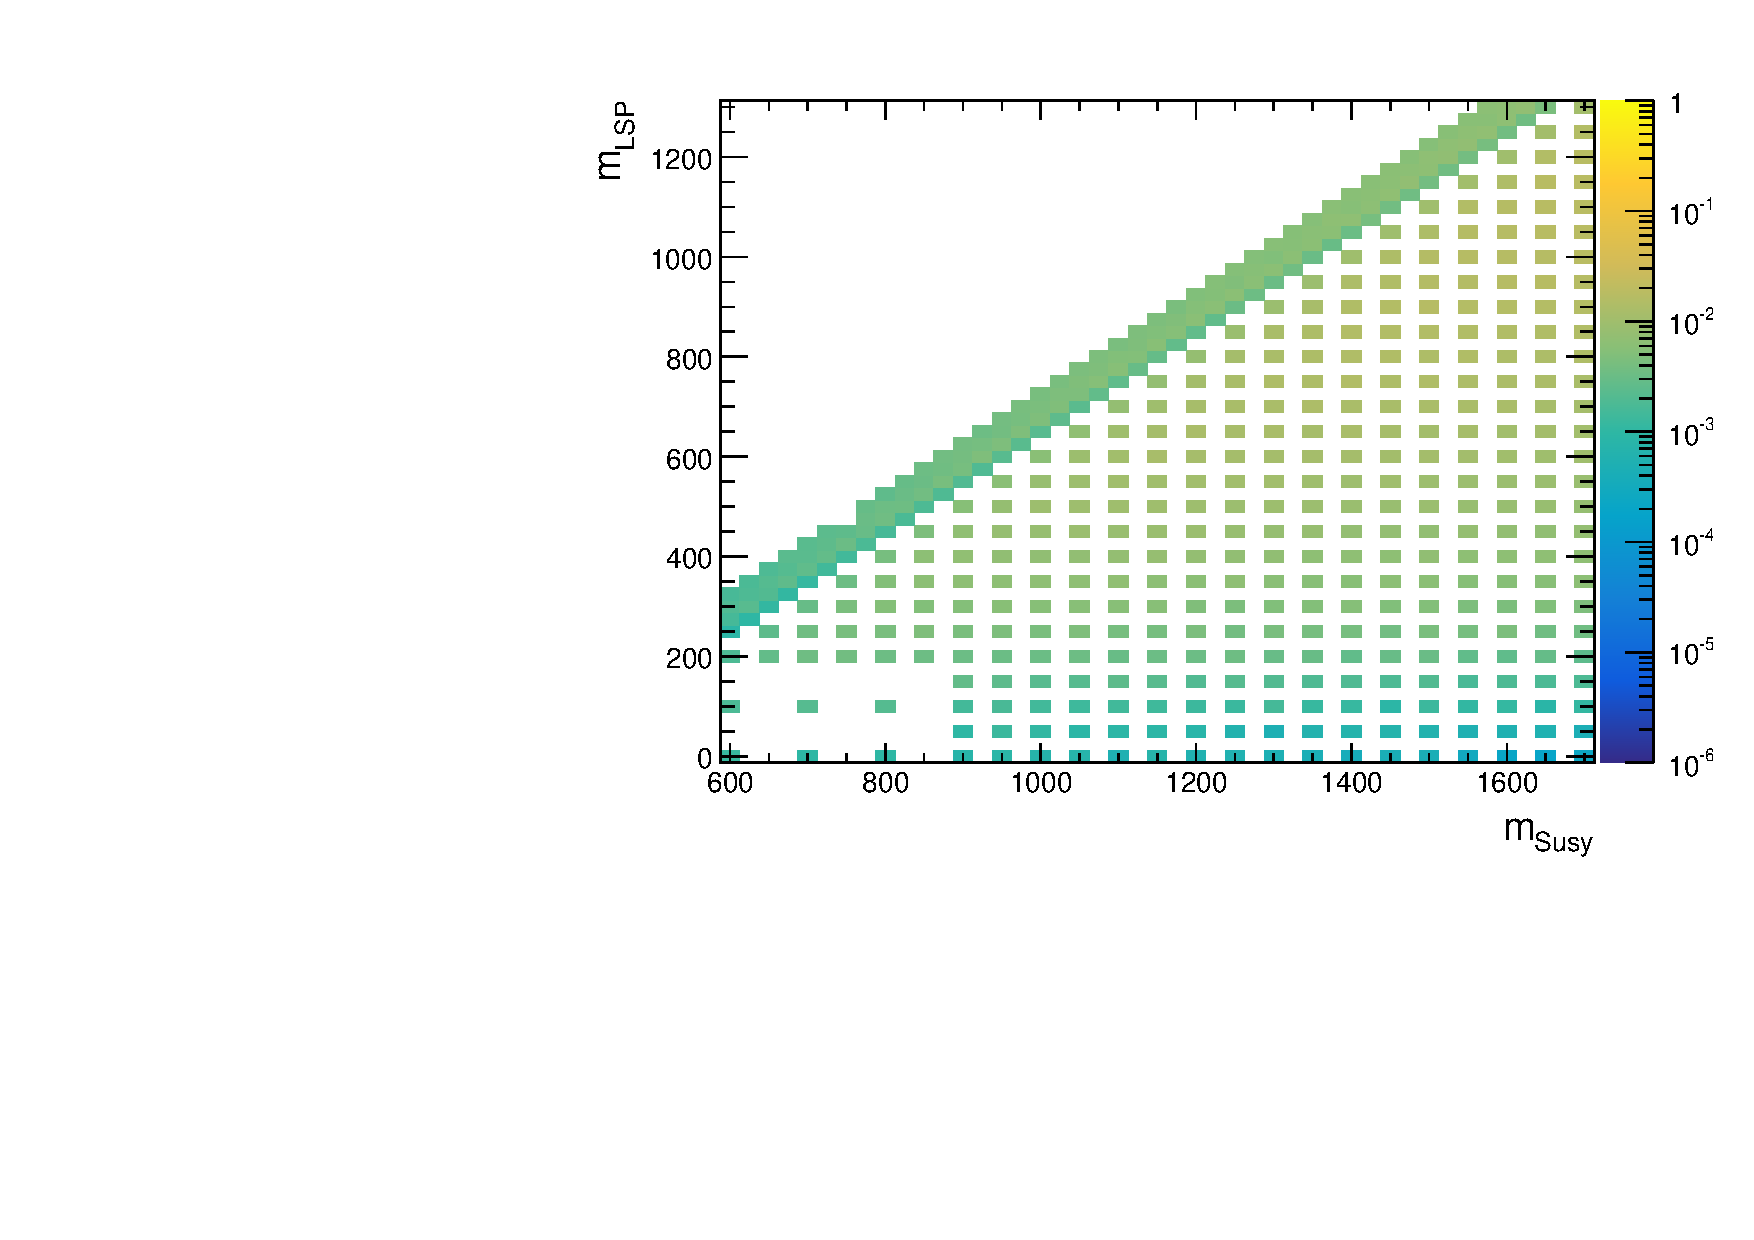
\includegraphics[width=0.45\textwidth]{figures/jetRanking/T5ttttDM175/eff/T5ttttDM175_merging_4_cats}
%%       \label{fig:T5ttttDM175_eff}
%%     } ~~
%%     \subfigure[T5ttttDM175: $\epsilon_{sig}^{\mathrm{4\,cat}}/\epsilon_{sig}^{\mathrm{tot}}$]{
%%       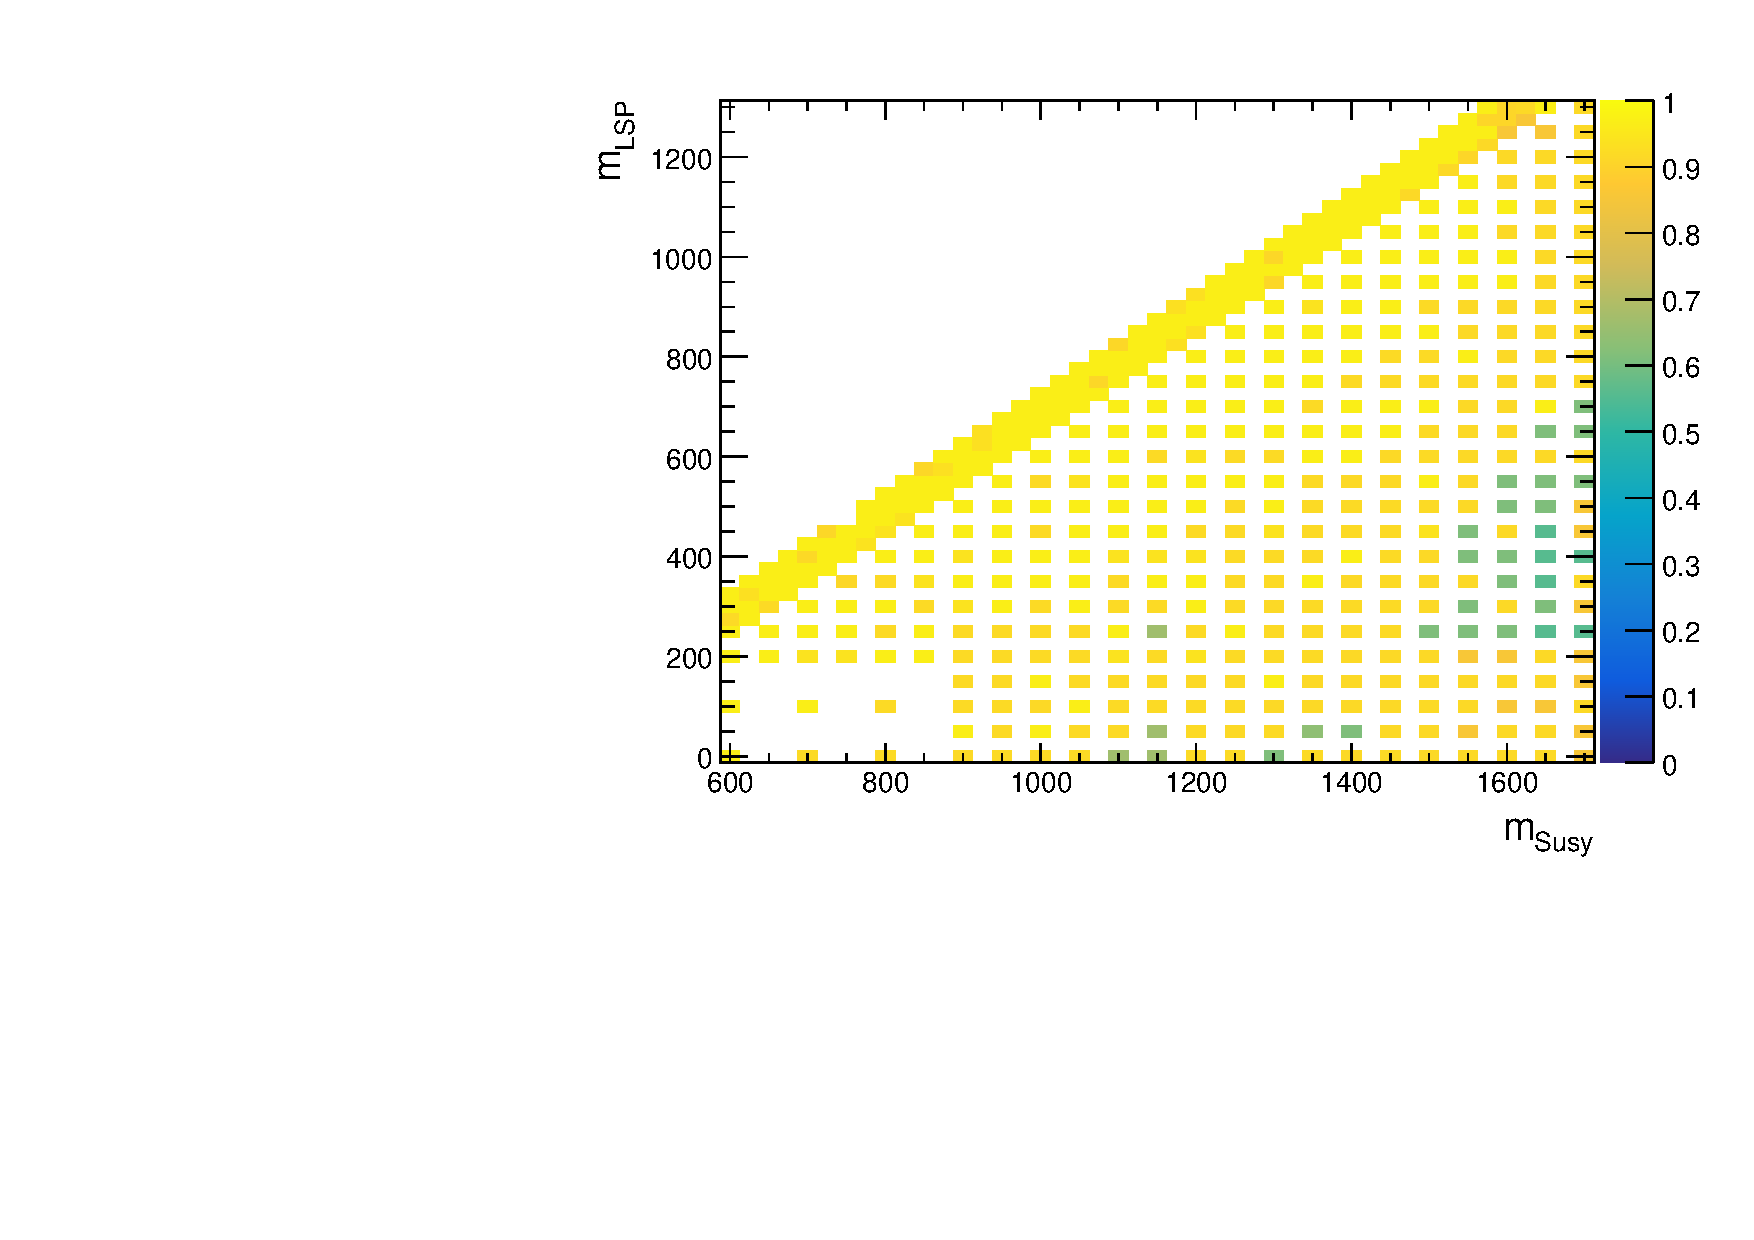
\includegraphics[width=0.45\textwidth]{figures/susyResults/T5ttttDM175_doubleRatioAcceptance}
%%       \label{fig:T5ttttDM175_eff_doubleRatio}
%%     }
%%     \caption{
%%       Top: the 95\% C.L. observed upper limit on the cross section (histogram), with the expected (solid black line) observed (solid red line) exclusion contours. 
%%       Bottom left: signal acceptance including the 4 most excluding jet categories. 
%%       Bottom right: ratio of the signal acceptance including 4 categories to the acceptance including the whole signal region. 
%%     }
%%     \label{fig:T5ttttDM175}
%%   \end{center}
%% \end{figure}



%% \newpage
%% \begin{figure}[h!]
%%   \begin{center}
%%     \subfigure[T5tttt\_degen: Upper limit on the cross section in the $(m_{\mathrm{Gluino}},m_{\mathrm{Susy}})$ plane]{
%%       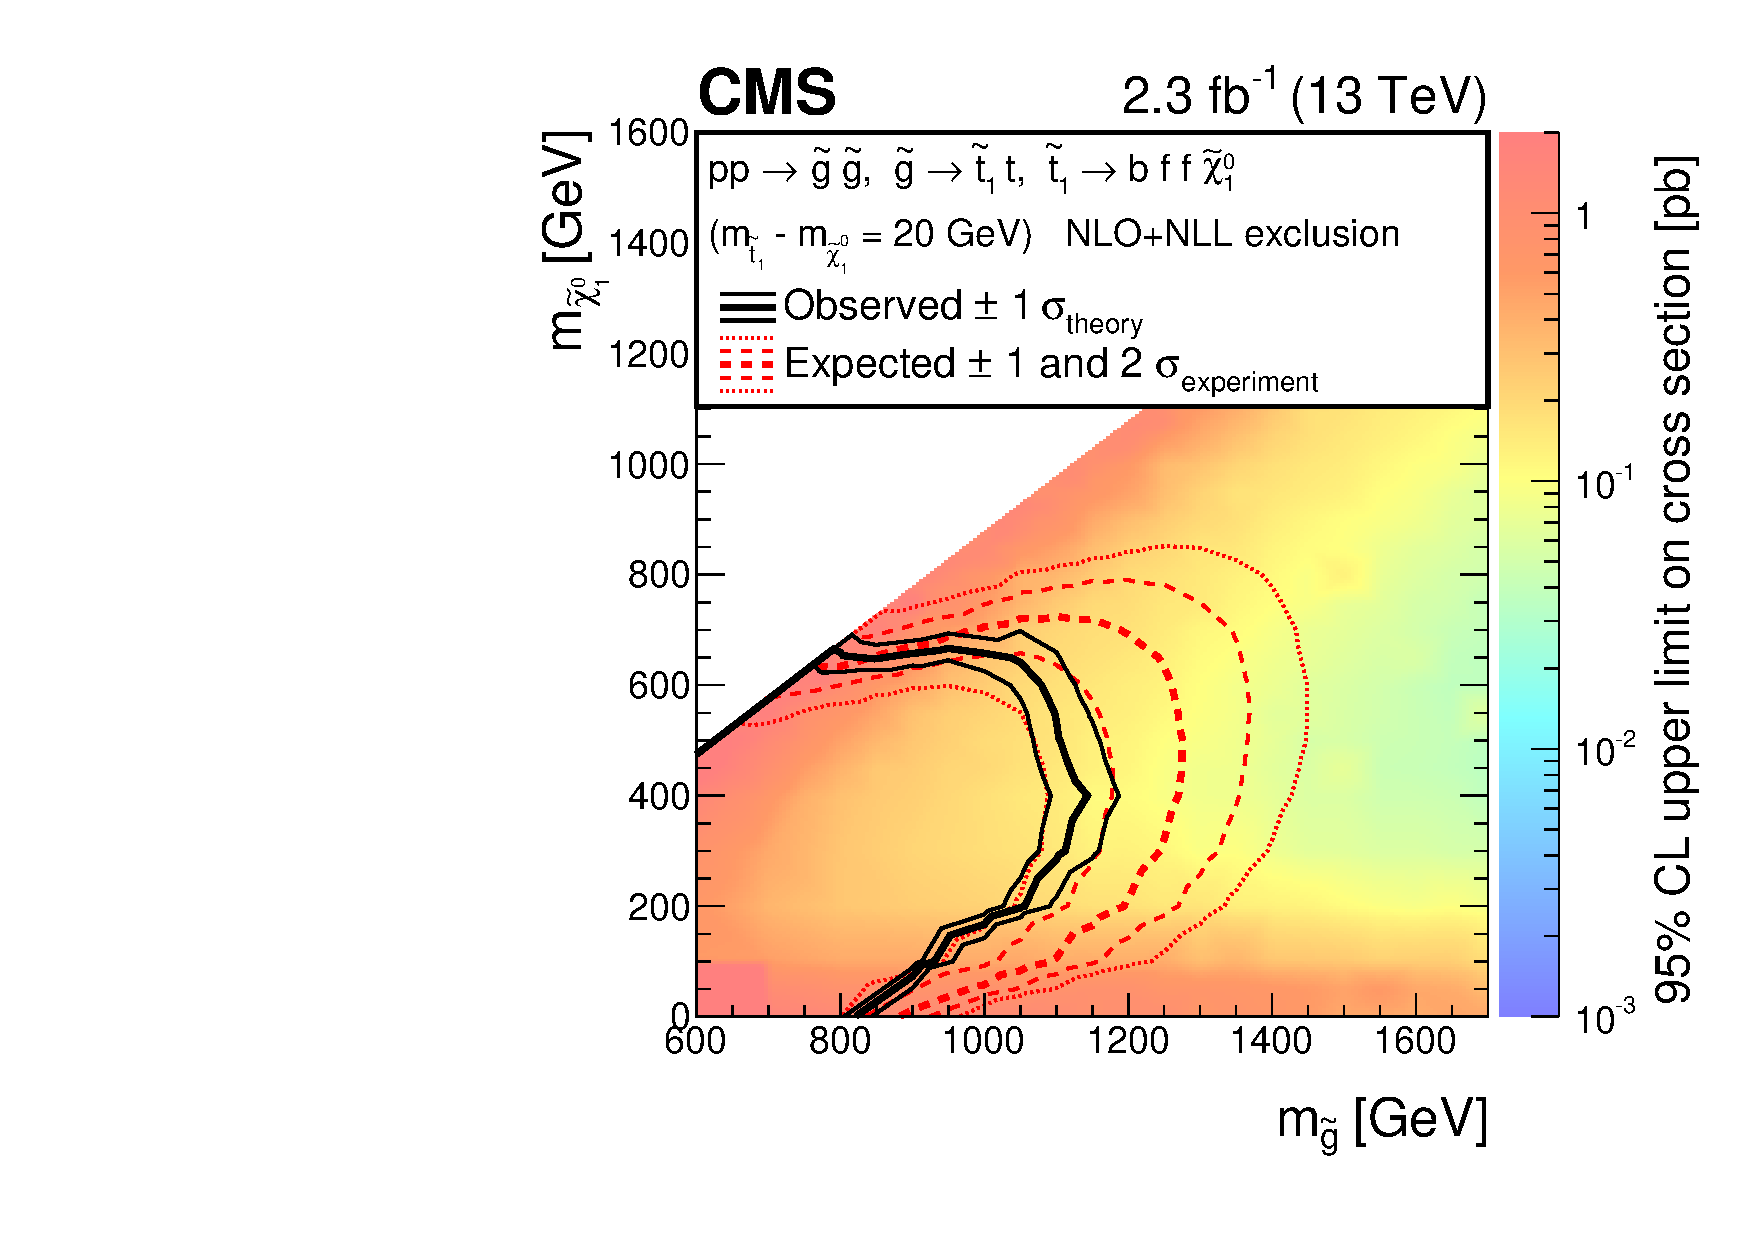
\includegraphics[width=0.6\textwidth]{figures/susyResults/T5tttt_degenXSEC}
%%       \label{fig:T5tttt_degen_excl}
%%     } \\
%%     \subfigure[T5tttt\_degen: $\epsilon_{sig}^{\mathrm{4\,cat}}$]{
%%       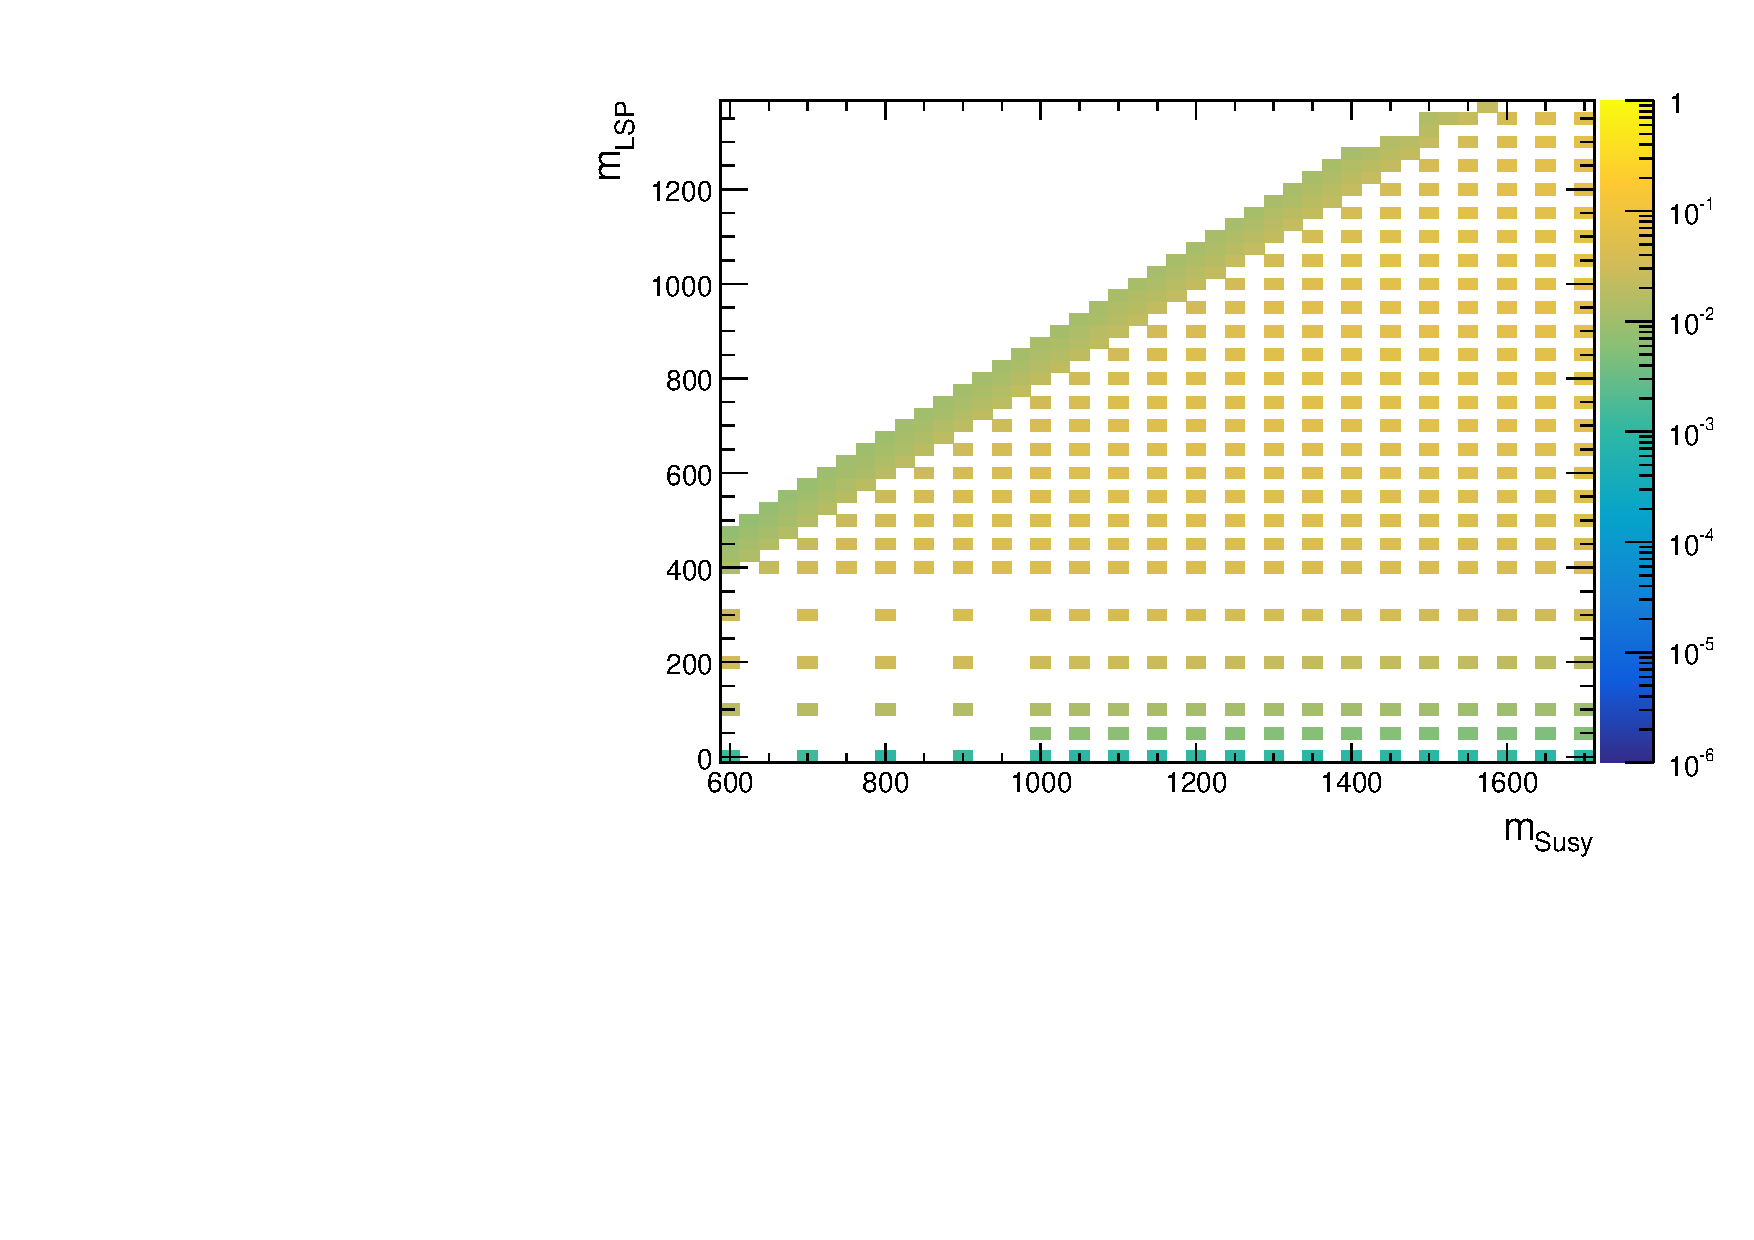
\includegraphics[width=0.45\textwidth]{figures/jetRanking/T5tttt_degen/eff/T5tttt_degen_merging_4_cats}
%%       \label{fig:T5tttt_degen_eff}
%%     } ~~
%%     \subfigure[T5tttt\_degen: $\epsilon_{sig}^{\mathrm{4\,cat}}/\epsilon_{sig}^{\mathrm{tot}}$]{
%%       \includegraphics[width=0.45\textwidth]{figures/susyResults/T5tttt_degen_doubleRatioAcceptance}
%%       \label{fig:T5tttt_degen_eff_doubleRatio}
%%     }
%%     \caption{
%%       Top: the 95\% C.L. observed upper limit on the cross section (histogram), with the expected (solid black line) observed (solid red line) exclusion contours. 
%%       Bottom left: signal acceptance including the 4 most excluding jet categories. 
%%       Bottom right: ratio of the signal acceptance including 4 categories to the acceptance including the whole signal region. 
%%     }
%%     \label{fig:T5tttt_degen}
%%   \end{center}
%% \end{figure}


%% \newpage
%% \begin{figure}[h!]
%%   \begin{center}
%%     \subfigure[T2tt: Upper limit on the cross section in the $(m_{\mathrm{Gluino}},m_{\mathrm{Susy}})$ plane]{
%%       \includegraphics[width=0.6\textwidth]{figures/susyResults/T2ttXSEC}
%%       \label{fig:T2tt_excl}
%%     } \\
%%     \subfigure[T2tt: $\epsilon_{sig}^{\mathrm{4\,cat}}$]{
%%       \includegraphics[width=0.45\textwidth]{figures/jetRanking/T2tt/eff/T2tt_merging_4_cats}
%%       \label{fig:T2tt_eff}
%%     } ~~
%%     \subfigure[T2tt: $\epsilon_{sig}^{\mathrm{4\,cat}}/\epsilon_{sig}^{\mathrm{tot}}$]{
%%       \includegraphics[width=0.45\textwidth]{figures/susyResults/T2tt_doubleRatioAcceptance}
%%       \label{fig:T2tt_eff_doubleRatio}
%%     }
%%     \caption{
%%       Top: the 95\% C.L. observed upper limit on the cross section (histogram), with the expected (solid black line) observed (solid red line) exclusion contours. 
%%       Bottom left: signal acceptance including the 4 most excluding jet categories. 
%%       Bottom right: ratio of the signal acceptance including 4 categories to the acceptance including the whole signal region. 
%%     }
%%     \label{fig:T2tt}
%%   \end{center}
%% \end{figure}


%% \newpage
%% \begin{figure}[h!]
%%   \begin{center}
%%     \subfigure[T2cc: Upper limit on the cross section in the $(m_{\mathrm{Gluino}},m_{\mathrm{Susy}})$ plane]{
%%       \includegraphics[width=0.6\textwidth]{figures/susyResults/T2ccXSEC}
%%       \label{fig:T2cc_excl}
%%     } \\
%%     \subfigure[T2cc: $\epsilon_{sig}^{\mathrm{4\,cat}}$]{
%%       \includegraphics[width=0.45\textwidth]{figures/jetRanking/T2cc/eff/T2cc_merging_4_cats}
%%       \label{fig:T2cc_eff}
%%     } ~~
%%     \subfigure[T2cc: $\epsilon_{sig}^{\mathrm{4\,cat}}/\epsilon_{sig}^{\mathrm{tot}}$]{
%%       \includegraphics[width=0.45\textwidth]{figures/susyResults/T2cc_doubleRatioAcceptance}
%%       \label{fig:T2cc_eff_doubleRatio}
%%     }
%%     \caption{
%%       Top: the 95\% C.L. observed upper limit on the cross section (histogram), with the expected (solid black line) observed (solid red line) exclusion contours. 
%%       Bottom left: signal acceptance including the 4 most excluding jet categories. 
%%       Bottom right: ratio of the signal acceptance including 4 categories to the acceptance including the whole signal region. 
%%     }
%%     \label{fig:T2cc}
%%   \end{center}
%% \end{figure}


%% \newpage
%% \begin{figure}[h!]
%%   \begin{center}
%%     \subfigure[T2-4bd: Upper limit on the cross section in the $(m_{\mathrm{Gluino}},m_{\mathrm{Susy}})$ plane]{
%%       \includegraphics[width=0.6\textwidth]{figures/susyResults/T2-4bdXSEC}
%%       \label{fig:T2-4bd_excl}
%%     } \\
%%     \subfigure[T2-4bd: $\epsilon_{sig}^{\mathrm{4\,cat}}$]{
%%       \includegraphics[width=0.45\textwidth]{figures/jetRanking/T2-4bd/eff/T2-4bd_merging_4_cats}
%%       \label{fig:T2-4bd_eff}
%%     } ~~
%%     \subfigure[T2-4bd: $\epsilon_{sig}^{\mathrm{4\,cat}}/\epsilon_{sig}^{\mathrm{tot}}$]{
%%       \includegraphics[width=0.45\textwidth]{figures/susyResults/T2-4bd_doubleRatioAcceptance}
%%       \label{fig:T2-4bd_eff_doubleRatio}
%%     }
%%     \caption{
%%       Top: the 95\% C.L. observed upper limit on the cross section (histogram), with the expected (solid black line) observed (solid red line) exclusion contours. 
%%       Bottom left: signal acceptance including the 4 most excluding jet categories. 
%%       Bottom right: ratio of the signal acceptance including 4 categories to the acceptance including the whole signal region. 
%%     }
%%     \label{fig:T2-4bd}
%%   \end{center}
%% \end{figure}


%% \newpage
%% \begin{figure}[h!]
%%   \begin{center}
%%     \subfigure[T2mixed: Upper limit on the cross section in the $(m_{\mathrm{Gluino}},m_{\mathrm{Susy}})$ plane]{
%%       \includegraphics[width=0.6\textwidth]{figures/susyResults/T2mixedXSEC}
%%       \label{fig:T2mixed_excl}
%%     } \\
%%     \subfigure[T2mixed: $\epsilon_{sig}^{\mathrm{4\,cat}}$]{
%%       \includegraphics[width=0.45\textwidth]{figures/jetRanking/T2mixed/eff/T2mixed_merging_4_cats}
%%       \label{fig:T2mixed_eff}
%%     } ~~
%%     \subfigure[T2mixed: $\epsilon_{sig}^{\mathrm{4\,cat}}/\epsilon_{sig}^{\mathrm{tot}}$]{
%%       \includegraphics[width=0.45\textwidth]{figures/susyResults/T2mixed_doubleRatioAcceptance}
%%       \label{fig:T2mixed_eff_doubleRatio}
%%     }
%%     \caption{
%%       Top: the 95\% C.L. observed upper limit on the cross section (histogram), with the expected (solid black line) observed (solid red line) exclusion contours. 
%%       Bottom left: signal acceptance including the 4 most excluding jet categories. 
%%       Bottom right: ratio of the signal acceptance including 4 categories to the acceptance including the whole signal region. 
%%     }
%%     \label{fig:T2mixed}
%%   \end{center}
%% \end{figure}


%% \newpage
%% \begin{figure}[h!]
%%   \begin{center}
%%     \subfigure[T2tb: Upper limit on the cross section in the $(m_{\mathrm{Gluino}},m_{\mathrm{Susy}})$ plane]{
%%       \includegraphics[width=0.6\textwidth]{figures/susyResults/T2tbXSEC}
%%       \label{fig:T2tb_excl}
%%     } \\
%%     \subfigure[T2tb: $\epsilon_{sig}^{\mathrm{4\,cat}}$]{
%%       \includegraphics[width=0.45\textwidth]{figures/jetRanking/T2tb/eff/T2tb_merging_4_cats}
%%       \label{fig:T2tb_eff}
%%     } ~~
%%     \subfigure[T2tb: $\epsilon_{sig}^{\mathrm{4\,cat}}/\epsilon_{sig}^{\mathrm{tot}}$]{
%%       \includegraphics[width=0.45\textwidth]{figures/susyResults/T2tb_doubleRatioAcceptance}
%%       \label{fig:T2tb_eff_doubleRatio}
%%     }
%%     \caption{
%%       Top: the 95\% C.L. observed upper limit on the cross section (histogram), with the expected (solid black line) observed (solid red line) exclusion contours. 
%%       Bottom left: signal acceptance including the 4 most excluding jet categories. 
%%       Bottom right: ratio of the signal acceptance including 4 categories to the acceptance including the whole signal region. 
%%     }
%%     \label{fig:T2tb}
%%   \end{center}
%% \end{figure}


%% \newpage
%% \begin{figure}[h!]
%%   \begin{center}
%%     \subfigure[T2bW\_X05: Upper limit on the cross section in the $(m_{\mathrm{Gluino}},m_{\mathrm{Susy}})$ plane]{
%%       \includegraphics[width=0.6\textwidth]{figures/susyResults/T2bW_X05XSEC}
%%       \label{fig:T2bW_X05_excl}
%%     } \\
%%     \subfigure[T2bW\_X05: $\epsilon_{sig}^{\mathrm{4\,cat}}$]{
%%       \includegraphics[width=0.45\textwidth]{figures/jetRanking/T2bW_X05/eff/T2bW_X05_merging_4_cats}
%%       \label{fig:T2bW_X05_eff}
%%     } ~~
%%     \subfigure[T2bW\_X05: $\epsilon_{sig}^{\mathrm{4\,cat}}/\epsilon_{sig}^{\mathrm{tot}}$]{
%%       \includegraphics[width=0.45\textwidth]{figures/susyResults/T2bW_X05_doubleRatioAcceptance}
%%       \label{fig:T2bW_X05_eff_doubleRatio}
%%     }
%%     \caption{
%%       Top: the 95\% C.L. observed upper limit on the cross section (histogram), with the expected (solid black line) observed (solid red line) exclusion contours. 
%%       Bottom left: signal acceptance including the 4 most excluding jet categories. 
%%       Bottom right: ratio of the signal acceptance including 4 categories to the acceptance including the whole signal region. 
%%     }
%%     \label{fig:T2bW_X05}
%%   \end{center}
%% \end{figure}



%% \newpage
%% \begin{figure}[h!]
%%   \begin{center}
%%     \subfigure[T2bb: Upper limit on the cross section in the $(m_{\mathrm{Gluino}},m_{\mathrm{Susy}})$ plane]{
%%       \includegraphics[width=0.6\textwidth]{figures/susyResults/T2bbXSEC}
%%       \label{fig:T2bb_excl}
%%     } \\
%%     \subfigure[T2bb: $\epsilon_{sig}^{\mathrm{4\,cat}}$]{
%%       \includegraphics[width=0.45\textwidth]{figures/jetRanking/T2bb/eff/T2bb_merging_4_cats}
%%       \label{fig:T2bb_eff}
%%     } ~~
%%     \subfigure[T2bb: $\epsilon_{sig}^{\mathrm{4\,cat}}/\epsilon_{sig}^{\mathrm{tot}}$]{
%%       \includegraphics[width=0.45\textwidth]{figures/susyResults/T2bb_doubleRatioAcceptance}
%%       \label{fig:T2bb_eff_doubleRatio}
%%     }
%%     \caption{
%%       Top: the 95\% C.L. observed upper limit on the cross section (histogram), with the expected (solid black line) observed (solid red line) exclusion contours. 
%%       Bottom left: signal acceptance including the 4 most excluding jet categories. 
%%       Bottom right: ratio of the signal acceptance including 4 categories to the acceptance including the whole signal region. 
%%     }
%%     \label{fig:T2bb}
%%   \end{center}
%% \end{figure}


%% \newpage
%% \begin{figure}[h!]
%%   \begin{center}
%%     \subfigure[T1qqqq: Upper limit on the cross section in the $(m_{\mathrm{Gluino}},m_{\mathrm{Susy}})$ plane]{
%%       \includegraphics[width=0.6\textwidth]{figures/susyResults/T1qqqqXSEC}
%%       \label{fig:T1qqqq_excl}
%%     } \\
%%     \subfigure[T1qqqq: $\epsilon_{sig}^{\mathrm{4\,cat}}$]{
%%       \includegraphics[width=0.45\textwidth]{figures/jetRanking/T1qqqq/eff/T1qqqq_merging_4_cats}
%%       \label{fig:T1qqqq_eff}
%%     } ~~
%%     \subfigure[T1qqqq: $\epsilon_{sig}^{\mathrm{4\,cat}}/\epsilon_{sig}^{\mathrm{tot}}$]{
%%       \includegraphics[width=0.45\textwidth]{figures/susyResults/T1qqqq_doubleRatioAcceptance}
%%       \label{fig:T1qqqq_eff_doubleRatio}
%%     }
%%     \caption{
%%       Top: the 95\% C.L. observed upper limit on the cross section (histogram), with the expected (solid black line) observed (solid red line) exclusion contours. 
%%       Bottom left: signal acceptance including the 4 most excluding jet categories. 
%%       Bottom right: ratio of the signal acceptance including 4 categories to the acceptance including the whole signal region. 
%%     }
%%     \label{fig:T1qqqq}
%%   \end{center}
%% \end{figure}


%% \newpage
%% \begin{figure}[h!]
%%   \begin{center}
%%     \subfigure[T2qq: Upper limit on the cross section in the $(m_{\mathrm{Gluino}},m_{\mathrm{Susy}})$ plane]{
%%       \includegraphics[width=0.6\textwidth]{figures/susyResults/T2qqXSEC}
%%       \label{fig:T2qq_excl}
%%     } \\
%%     \subfigure[T2qq: $\epsilon_{sig}^{\mathrm{4\,cat}}$]{
%%       \includegraphics[width=0.45\textwidth]{figures/jetRanking/T2qq/eff/T2qq_merging_4_cats}
%%       \label{fig:T2qq_eff}
%%     } ~~
%%     \subfigure[T2qq: $\epsilon_{sig}^{\mathrm{4\,cat}}/\epsilon_{sig}^{\mathrm{tot}}$]{
%%       \includegraphics[width=0.45\textwidth]{figures/susyResults/T2qq_doubleRatioAcceptance}
%%       \label{fig:T2qq_eff_doubleRatio}
%%     }
%%     \caption{
%%       Top: the 95\% C.L. observed upper limit on the cross section (histogram), with the expected (solid black line) observed (solid red line) exclusion contours. 
%%       Bottom left: signal acceptance including the 4 most excluding jet categories. 
%%       Bottom right: ratio of the signal acceptance including 4 categories to the acceptance including the whole signal region. 
%%     }
%%     \label{fig:T2qq}
%%   \end{center}
%% \end{figure}


%% \begin{figure*}[thp!]
%%   \begin{center}
%%     \includegraphics[width=0.49\textwidth]{figures/susyResults/mixSUMMARY.pdf}
%%     \includegraphics[width=0.49\textwidth]{figures/susyResults/gluinoSUMMARY.pdf} \\
%%     \includegraphics[width=0.49\textwidth]{figures/susyResults/naturalSUMMARY.pdf}
%%     \includegraphics[width=0.49\textwidth]{figures/susyResults/allThirdGenSUMMARY.pdf} \\
%%     \caption{Summary for the observed (solid lines) and expected (dashed lines) exclusions in the $m_{\mathrm{Susy}},m_{\mathrm{LSP}}$ plane for the models considered in the analysis. 
%%        Exclusion contours are grouped into 4 summary plots according to the categorisation presented at the begin of Sec.~\ref{sec:susy_results}: 
%%        ``Direct and gluino-mediated production of off-shell (decoupled) light-flavour squarks'' (top left), ``Gluino-mediated production of off-shell (decoupled) 3rd generation squarks'' (top right), ``Gluino-mediated production of on-shell stops and charginos (natural models)'' (bottom left), ``Direct production of 3rd generation squarks'' (bottom right). 
%%       \label{fig:summary-excl-plots} }
%%   \end{center}
%% \end{figure*}


%% \newpage
%% Gluino masses up to $\sim$1550 GeV are excluded (T1bbbb). 
%% Stop production is excluded up to $\sim$660 GeV in the 2-body decay to top quarks (T2tt), 
%% and up to $\sim$370 GeV in the compressed region, in the decay to charm quarks (T2cc). 
%% Sbottom (squark) masses smaller than $\sim$800 GeV ($\sim$600 GeV) are excluded for small LSP masses (T2bb,T2qq). 
%% In the case of squark decaying to light quarks, the exclusion reaches $\sim$1150 GeV when assuming degeneracy of 
%% all the first and second generation squarks. \\
%% For most of the models considered, the exclusion exceeds the one of the 8 TeV data. 

%% A moderate excess in the $\njet\geq5, \nb\geq2, \scalht > 800 \, \mathrm{GeV}$ (see Tab.~\ref{tab:predallqcdpost_sig_comb_sym})
%% causes the observed limits to be slightly weaker than expected for the models favouring high \nb, high \nj and high \scalht. \\
%% In Tab.~\ref{tab:sigBenchmarksYields_excess} some benchmark points for different models are listed, 
%% which are expected to be excluded by this search but are not with the current dataset, due to this excess. \\
%% For T1tttt, T5ttttDM175 this excess has a more pronounced effect in the limit and the observed limit is $\sim 2\sigma$ 
%% weaker than expected. The cause of this weaker than expected trend has been studied in more detail
%% and localised to a fluctuation in these analysis bins. Event displays for collision events 
%% falling in these analysis bins have been carefully inspected and are do not exhibit any 
%% significant problems, thus making us confident that they are real physics events. 

\subsection{Signal model sensitivity tables}
\label{sec:lim-sum-tables}

Tables~\ref{tab:benchMarkTable_T2tt}-\ref{tab:benchMarkTable_T1bbbb} show the overall limits 
for benchmark SUSY limits as well as the limits for the most sensitive categories alone.
The predictions and obersvations in these categories are also given.
The \mht dimension is used when making the limits for these bins. 

\begin{landscape}
\begin{longtable}{ccccccc}
\caption{Expected and observed limits for most sensitive categories for benchmark models} \label{tab:benchMarkTable_T2tt} \\    \hline
Signal Model & Rank (by expected limit) & Category & Prediction & Observation & Expected limit & Observed limit\\ \hline
T2tt (300,200) & 1 & $\ge5$j, 1b, $800-\inf$ & $172.67 \pm 34.36$ & 141 & 3.39 & 2.86\\ 
T2tt (300,200) & 2 & $\ge5$j, 0b, $600-800$ & $405.83 \pm 19.42$ & 402 & 3.55 & 2.80\\ 
T2tt (300,200) & 3 & $\ge5$j, 0b, $500-600$ & $394.63 \pm 53.22$ & 443 & 4.02 & 2.80\\ 
T2tt (300,200) & 4 & $\ge5$a, 0b, $400-500$ & $478.43 \pm 50.73$ & 528 & 4.23 & 8.12\\ 
T2tt (300,200) & 5 & $\ge5$a, 0b, $500-600$ & $99.97 \pm 7.00$ & 95 & 4.80 & 5.65\\ 
T2tt (300,200) & All & - & - & - & 1.00 & 1.64\\ 
T2tt (900,1) & 1 & $\ge5$j, 2b, $800-\inf$ & $64.95 \pm 13.17$ & 49 & 1.76 & 2.91\\ 
T2tt (900,1) & 2 & $\ge5$j, 1b, $800-\inf$ & $172.67 \pm 34.36$ & 141 & 2.16 & 2.32\\ 
T2tt (900,1) & 3 & $\ge5$j, $\ge3$b, $800-\inf$ & $8.98 \pm 1.03$ & 9 & 3.67 & 3.26\\ 
T2tt (900,1) & 4 & 4j, 2b, $800-\inf$ & $13.77 \pm 1.31$ & 12 & 4.11 & 2.78\\ 
T2tt (900,1) & 5 & $\ge5$j, 2b, $600-800$ & $74.75 \pm 11.00$ & 66 & 5.11 & 4.80\\ 
T2tt (900,1) & All & - & - & - & 0.93 & 1.26\\ 
\hline
\hline
\end{longtable}
\end{landscape}

\clearpage
\begin{landscape}
\begin{longtable}{ccccccc}
\caption{Expected and observed limits for most sensitive categories for benchmark models} \label{tab:benchMarkTable_T2qq} \\    \hline
Signal Model & Rank (by expected limit) & Category & Prediction & Observation & Expected limit & Observed limit\\ \hline
T2qq (400,350) & 1 & $\ge5$j, 0b, $600-800$ & $405.83 \pm 19.42$ & 402 & 2.18 & 2.70\\ 
T2qq (400,350) & 2 & $\ge5$j, 0b, $800-\inf$ & $336.97 \pm 14.29$ & 344 & 2.18 & 2.06\\ 
T2qq (400,350) & 3 & $\ge5$j, 1b, $800-\inf$ & $172.67 \pm 34.36$ & 141 & 3.31 & 5.27\\ 
T2qq (400,350) & 4 & $\ge5$j, 0b, $500-600$ & $394.63 \pm 53.22$ & 443 & 3.86 & 4.62\\ 
T2qq (400,350) & 5 & $\ge5$a, 0b, $400-500$ & $478.43 \pm 50.73$ & 528 & 4.16 & 5.40\\ 
T2qq (400,350) & All & - & - & - & 0.80 & 1.46\\ 
T2qq (500,350) & 1 & $\ge5$j, 0b, $600-800$ & $405.83 \pm 19.42$ & 402 & 2.46 & 2.79\\ 
T2qq (500,350) & 2 & $\ge5$j, 0b, $800-\inf$ & $336.97 \pm 14.29$ & 344 & 3.06 & 3.18\\ 
T2qq (500,350) & 3 & $\ge5$j, 0b, $500-600$ & $394.63 \pm 53.22$ & 443 & 3.96 & 4.93\\ 
T2qq (500,350) & 4 & 4j, 0b, $600-800$ & $516.81 \pm 24.62$ & 521 & 4.32 & 4.27\\ 
T2qq (500,350) & 5 & $\ge5$j, 1b, $800-\inf$ & $172.67 \pm 34.36$ & 141 & 4.92 & 5.37\\ 
T2qq (500,350) & All & - & - & - & 0.93 & 1.77\\ 
T2qq (800,1) & 1 & $\ge5$j, 0b, $800-\inf$ & $336.97 \pm 14.29$ & 344 & 2.37 & 1.59\\ 
T2qq (800,1) & 2 & 2j, 0b, $800-\inf$ & $392.70 \pm 84.24$ & 345 & 2.49 & 1.66\\ 
T2qq (800,1) & 3 & 4j, 0b, $800-\inf$ & $381.84 \pm 26.44$ & 391 & 2.96 & 1.79\\ 
T2qq (800,1) & 4 & 3j, 0b, $800-\inf$ & $503.41 \pm 37.12$ & 519 & 3.45 & 1.97\\ 
T2qq (800,1) & 5 & 2j, 0b, $600-800$ & $309.71 \pm 13.55$ & 303 & 5.02 & 4.40\\ 
T2qq (800,1) & All & - & - & - & 1.07 & 0.85\\ 
\hline
\hline
\end{longtable}
\end{landscape}

\clearpage
\begin{landscape}
\begin{longtable}{ccccccc}
\caption{Expected and observed limits for most sensitive categories for benchmark models} \label{tab:benchMarkTable_T2bb} \\    \hline
Signal Model & Rank (by expected limit) & Category & Prediction & Observation & Expected limit & Observed limit\\ \hline
T2bb (1000,1) & 1 & 2j, 2b, $600-\inf$ & $2.36 \pm 0.74$ & 1 & 2.50 & 1.91\\ 
T2bb (1000,1) & 2 & 3j, 2b, $800-\inf$ & $10.96 \pm 1.76$ & 5 & 3.01 & 1.70\\ 
T2bb (1000,1) & 3 & 2j, 1b, $800-\inf$ & $35.88 \pm 2.95$ & 40 & 3.20 & 4.52\\ 
T2bb (1000,1) & 4 & 4j, 2b, $800-\inf$ & $13.77 \pm 1.31$ & 12 & 4.11 & 2.86\\ 
T2bb (1000,1) & 5 & 3j, 1b, $800-\inf$ & $94.96 \pm 20.02$ & 83 & 4.27 & 2.27\\ 
T2bb (1000,1) & All & - & - & - & 1.07 & 0.80\\ 
T2bb (450,400) & 1 & $\ge5$j, 1b, $800-\inf$ & $172.67 \pm 34.36$ & 141 & 2.20 & 2.47\\ 
T2bb (450,400) & 2 & $\ge5$j, 2b, $800-\inf$ & $64.95 \pm 13.17$ & 49 & 3.77 & 4.58\\ 
T2bb (450,400) & 3 & 4j, 1b, $800-\inf$ & $113.11 \pm 8.57$ & 107 & 4.30 & 4.59\\ 
T2bb (450,400) & 4 & $\ge5$j, 1b, $600-800$ & $186.88 \pm 9.85$ & 181 & 4.73 & 4.26\\ 
T2bb (450,400) & 5 & 4j, 1b, $600-800$ & $125.90 \pm 18.15$ & 127 & 5.30 & 6.09\\ 
T2bb (450,400) & All & - & - & - & 0.93 & 0.72\\ 
\hline
\hline
\end{longtable}
\end{landscape}

\clearpage
\begin{landscape}
\begin{longtable}{ccccccc}
\caption{Expected and observed limits for most sensitive categories for benchmark models} \label{tab:benchMarkTable_T1tttt} \\    \hline
Signal Model & Rank (by expected limit) & Category & Prediction & Observation & Expected limit & Observed limit\\ \hline
T1tttt (1600,1) & 1 & $\ge5$j, $\ge3$b, $800-\inf$ & $8.98 \pm 1.03$ & 9 & 1.54 & 1.34\\ 
T1tttt (1600,1) & 2 & $\ge5$j, 2b, $800-\inf$ & $64.95 \pm 13.17$ & 49 & 2.77 & 5.86\\ 
T1tttt (1600,1) & 3 & $\ge5$j, 1b, $800-\inf$ & $172.67 \pm 34.36$ & 141 & 9.03 & 9.48\\ 
T1tttt (1600,1) & 4 & $\ge5$j, 0b, $800-\inf$ & $336.97 \pm 14.29$ & 344 & 48.38 & 23.33\\ 
T1tttt (1600,1) & 5 & 4j, 2b, $800-\inf$ & $13.77 \pm 1.31$ & 12 & 254.25 & 213.42\\ 
T1tttt (1600,1) & All & - & - & - & 1.15 & 2.36\\ 
T1tttt (800,575) & 1 & $\ge5$j, 1b, $800-\inf$ & $172.67 \pm 34.36$ & 141 & 1.73 & 2.68\\ 
T1tttt (800,575) & 2 & $\ge5$j, 0b, $800-\inf$ & $336.97 \pm 14.29$ & 344 & 2.98 & 4.66\\ 
T1tttt (800,575) & 3 & $\ge5$a, 0b, $600-\inf$ & $21.49 \pm 2.12$ & 26 & 3.70 & 4.75\\ 
T1tttt (800,575) & 4 & $\ge5$a, 1b, $600-\inf$ & $12.39 \pm 3.98$ & 12 & 3.89 & 3.73\\ 
T1tttt (800,575) & 5 & $\ge5$a, 0b, $500-600$ & $99.97 \pm 7.00$ & 95 & 3.92 & 4.69\\ 
T1tttt (800,575) & All & - & - & - & 0.79 & 1.38\\ 
\hline
\hline
\end{longtable}
\end{landscape}

\clearpage
\begin{landscape}
\begin{longtable}{ccccccc}
\caption{Expected and observed limits for most sensitive categories for benchmark models} \label{tab:benchMarkTable_T1qqqq} \\    \hline
Signal Model & Rank (by expected limit) & Category & Prediction & Observation & Expected limit & Observed limit\\ \hline
T1qqqq (1000,900) & 1 & $\ge5$j, 0b, $800-\inf$ & $336.97 \pm 14.29$ & 344 & 2.02 & 1.44\\ 
T1qqqq (1000,900) & 2 & $\ge5$j, 1b, $800-\inf$ & $172.67 \pm 34.36$ & 141 & 3.17 & 3.81\\ 
T1qqqq (1000,900) & 3 & $\ge5$j, 0b, $600-800$ & $405.83 \pm 19.42$ & 402 & 3.30 & 4.08\\ 
T1qqqq (1000,900) & 4 & $\ge5$a, 0b, $600-\inf$ & $21.49 \pm 2.12$ & 26 & 3.52 & 3.98\\ 
T1qqqq (1000,900) & 5 & 4j, 0b, $800-\inf$ & $381.84 \pm 26.44$ & 391 & 5.36 & 3.37\\ 
T1qqqq (1000,900) & All & - & - & - & 0.95 & 1.33\\ 
T1qqqq (1600,1) & 1 & $\ge5$j, 0b, $800-\inf$ & $336.97 \pm 14.29$ & 344 & 1.54 & 0.73\\ 
T1qqqq (1600,1) & 2 & $\ge5$j, 1b, $800-\inf$ & $172.67 \pm 34.36$ & 141 & 2.80 & 2.21\\ 
T1qqqq (1600,1) & 3 & 4j, 0b, $800-\inf$ & $381.84 \pm 26.44$ & 391 & 4.08 & 3.39\\ 
T1qqqq (1600,1) & 4 & $\ge5$j, 2b, $800-\inf$ & $64.95 \pm 13.17$ & 49 & 8.47 & 18.37\\ 
T1qqqq (1600,1) & 5 & 4j, 1b, $800-\inf$ & $113.11 \pm 8.57$ & 107 & 9.34 & 7.84\\ 
T1qqqq (1600,1) & All & - & - & - & 1.14 & 0.70\\ 
\hline
\hline
\end{longtable}
\end{landscape}

\clearpage
\begin{landscape}
\begin{longtable}{ccccccc}
\caption{Expected and observed limits for most sensitive categories for benchmark models} \label{tab:benchMarkTable_T1bbbb} \\    \hline
Signal Model & Rank (by expected limit) & Category & Prediction & Observation & Expected limit & Observed limit\\ \hline
T1bbbb (1000,900) & 1 & $\ge5$j, 2b, $800-\inf$ & $64.95 \pm 13.17$ & 49 & 1.21 & 1.87\\ 
T1bbbb (1000,900) & 2 & $\ge5$j, $\ge3$b, $800-\inf$ & $8.98 \pm 1.03$ & 9 & 1.39 & 1.41\\ 
T1bbbb (1000,900) & 3 & $\ge5$j, 1b, $800-\inf$ & $172.67 \pm 34.36$ & 141 & 1.99 & 2.19\\ 
T1bbbb (1000,900) & 4 & $\ge5$j, 2b, $600-800$ & $74.75 \pm 11.00$ & 66 & 2.37 & 1.68\\ 
T1bbbb (1000,900) & 5 & $\ge5$j, $\ge3$b, $600-800$ & $11.36 \pm 1.93$ & 14 & 2.71 & 3.34\\ 
T1bbbb (1000,900) & All & - & - & - & 0.44 & 0.48\\ 
T1bbbb (1800,1) & 1 & $\ge5$j, $\ge3$b, $800-\inf$ & $8.98 \pm 1.03$ & 9 & 1.71 & 1.44\\ 
T1bbbb (1800,1) & 2 & $\ge5$j, 2b, $800-\inf$ & $64.95 \pm 13.17$ & 49 & 2.20 & 5.53\\ 
T1bbbb (1800,1) & 3 & 4j, 2b, $800-\inf$ & $13.77 \pm 1.31$ & 12 & 5.48 & 5.11\\ 
T1bbbb (1800,1) & 4 & 4j, $\ge3$b, $800-\inf$ & $2.63 \pm 1.03$ & 0 & 6.47 & 5.04\\ 
T1bbbb (1800,1) & 5 & $\ge5$j, 1b, $800-\inf$ & $172.67 \pm 34.36$ & 141 & 8.53 & 7.13\\ 
T1bbbb (1800,1) & All & - & - & - & 0.93 & 1.49\\ 
\hline
\hline
\end{longtable}
\end{landscape}





%%____________________________________________________________________________||
